
%input macros (i.e. write your own macros file called MacroFile1.tex)
%\include{Macros/MacroFile1}

\documentclass[oneside,12pt]{Classes/CUEDthesisPSnPDF}
\usepackage{amsmath}
\usepackage{latexsym}
\usepackage{graphicx}
\usepackage{float}
\usepackage{booktabs}
\usepackage{listings}
\usepackage{overcite}
\usepackage{pgf}
\usepackage{multirow}

\renewcommand\citeleft{[}  % parentheses around list
\renewcommand\citeright{]} % parentheses around list

\ifpdf
    \pdfinfo { /Title  (Internship Report)
               /Creator (Jianhui Yang)
              /Producer (pdfTeX)
               /Author (Jianhui Yang Jianhui.yang@eleves.nantes.fr)
               /CreationDate (D:20100601000000)  %format D:YYYYMMDDhhmmss
               /ModDate (D:20100601213532)
               /Subject (Simulation of a Mars Rover on granular soils)
               /Keywords (MSc, Thesis)}
    \pdfcatalog { /PageMode (/UseOutlines)
                  /OpenAction (fitbh)  }
\fi

\title{\Huge Simulation of a Mars Rover on granular soils}

\ifpdf
  \author{\href{dd}}
  \collegeordept{\href{http://www.inrialpes.fr}{Team Bipop}}
  \university{\href{http://www.inrialpes.fr}{INRIA Rh\^one Alpes}}
% insert below the file name that contains the crest in-place of 'UnivShield'
  \crest{
\includegraphics[width=60mm]{INRIA}}
\else
  \author{Jianhui Yang}
  \collegeordept{\normalsize Supervisor: Vincent Acary\\Team Bipop }
  \university{\normalsize INRIA Rh\^one Alpes }
% insert below the file name that contains the crest in-place of 'UnivShield'
  \crest{
\includegraphics[width=60mm]{INRIA}}
\fi



%
% insert below the file name that contains the crest in-place of 'LOGO CENTRALE NANTES'
% \crest{\IncludeGraphicsW{LOGO CENTRALE NANTES}{40mm}{14 14 73 81}}

\renewcommand{\submittedtext}{A internship report submitted for}
\degree{Erasmus Mundus Master} \degreedate{14 June 2010}

% turn of those nasty overfull and underfull hboxes
\hbadness=10000
\hfuzz=50pt

% Put all the style files you want in the directory StyleFiles and usepackage like this:
\usepackage{StyleFiles/watermark}


\begin{document}

%\language{english}

 \renewcommand\baselinestretch{1.2}
\baselineskip=18pt plus1pt

% A page with the abstract on including title and author etc may be
% required to be handed in separately. If this is not so, then comment
% the below 3 lines (between '\begin{abstractseparte}' and
% 'end{abstractseparate}'), normally like a declaration ... needs some more
% work, mind as environment abstracts creates a new page!
% \begin{abstractseparate}
%   \input{Abstract/abstract}
% \end{abstractseparate}




% Using the watermark package which is in StyleFiles/
% and to remove DRAFT COPY ONLY appearing on the top of all pages comment out below line
%\watermark{DRAFT COPY ONLY}


\maketitle

%set the number of sectioning levels that get number and appear in the contents
\setcounter{secnumdepth}{3}
\setcounter{tocdepth}{3}

\frontmatter
%\include{Dedication/dedication}
%\include{Acknowledgement/acknowledgement}
%\include{Abstract/abstract}

\tableofcontents
\listoffigures
%\printglossary  %% Print the nomenclature
%\addcontentsline{toc}{chapter}{Nomenclature} %-------------


%\include{Introduction/introduction}

\mainmatter


\chapter{Introduction of INRIA Rh\^one Alpes and Team Bipop}
\ifpdf
    \graphicspath{{Chapter1/Chapter1Figs/PNG/}{Chapter1/Chapter1Figs/PDF/}{Chapter1/Chapter1Figs/}}
\else
    \graphicspath{{Chapter1/Chapter1Figs/EPS/}{Chapter1/Chapter1Figs/}}
\fi


\section{INRIA Rh\^one Alpes}

INRIA Grenoble - Rh\^one-Alpes Research Centre is one of the eight research centres run by INRIA, the French National Institute for Research in Computer Science and Control. As a public institute jointly supervised by the French Ministries of Research and of Industry, the centre aims to fulfil two key duties:

\begin{itemize}
\item To carry out fundamental and applied research in information and communication science and technology (ICST).
\item To share its research results and promote their application in society.
\end{itemize}

And there are some useful key points for INRIA Rh\^one Alpes:

\begin{itemize}
\item  Founded in: 1992
\item Approximately 600 people, half of whom are on INRIA's payroll and a third of whom are doctoral students
\item 28 research teams
\item Research support departments
\item Approximately 50\% of its budget comes from contracted project funding.
\end{itemize}

\section{Team Bipop}

Team Bipop is concerned with non-smooth dynamical systems and non-smooth optimization. More precisely, modelling, control and numerical simulation are the main scientific topics. The basic tools therefore come from non-smooth mechanics, systems and control theory, non-smooth optimisation, and convex and non-smooth analysis.\\



The main applications can be found in mechanical systems (multibody systems with unilateral constraints, friction, nonsmooth contact laws), and in electrical systems (circuits with diodes, MOS transistors). Some more abstract problems (like optimal control with state constraints, generalized predictive control) also fit within this framework.\\

The main areas of application are: automotive systems, aerospace applications, electro-mechanical systems (mechatronics), robotics, etc. There are still many open fields of theoretical research (in systems theory: controllability, observability, stabilisation, trajectory tracking; in mechanical modelling: multiple impacts modelling, nonmonotone contact laws, Painlevé paradoxes), as well as on a more applied level (numerical simulation and software development). The biped robot is one of the many applications for control and simulation.\\


\section{Short introduction of the Siconos Platform}

The Siconos Platform is a scientific computing software dedicated to the modeling, simulation, control and analysis of Non Smooth Dynamical Systems (NSDS). Especially, the following classes of NSDS are addressed:

\begin{itemize}
\item Mechanical systems with contact, impact and friction
\item Electrical circuits with ideal and piecewise linear components
\item Differential inclusions and Complementarity systems
\end{itemize}







\chapter{Project description}
\ifpdf
    \graphicspath{{Chapter2/PNG/}{Chapter2/PDF/}{Chapter2/}}
\else
    \graphicspath{{Chapter2/Chapter2Figs/EPS/}{Chapter2/}}
\fi

This internship is taken place within the project Bipop whose research topic is the study of
nonsmooth dynamical systems. It is part of a collaboration with the company
Trasys contracting the European Space Agency (ESA), in particular, has developed a Trasys
3D simulation software of a Mars Rover: 3DROV. Bipop develops a software platform SICONOS for
simulation of nonsmooth dynamic systems, especially mechanical systems. Better friction-contact models could be involved in Siconos to improve the existing simulation in 3DROV\\

The objective of the course internship is to integrate the simulation engine in the tool SICONOS
visualization 3DROV ESA and test simulations of moving a Rover Mars on a granular soil.

\begin{figure}[H]
 \begin{center}
      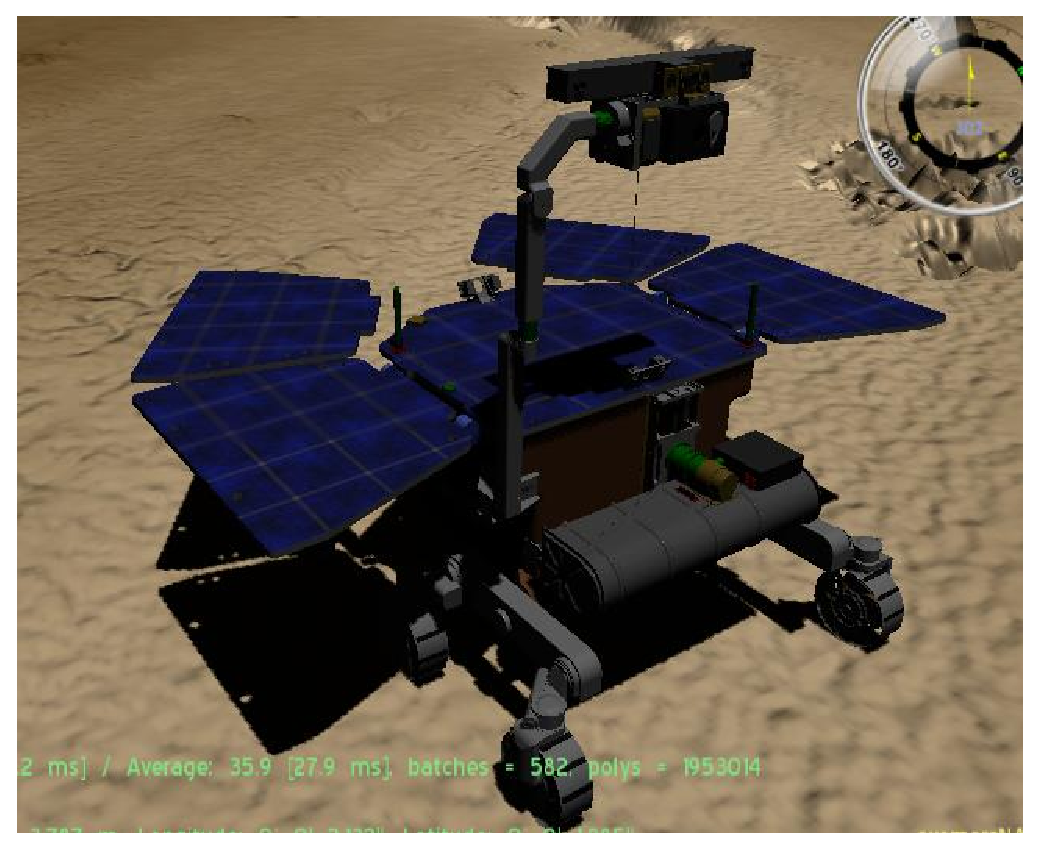
\includegraphics[width=8cm]{stage.EPS}
  \end{center}
\end{figure}


The main objectives of the internship are:

\begin{itemize}
\item Learning to use the platform SICONOS, dynamics and non-regular
models of contact friction
\item Create a 2D model to simulate Rover on granular soil.
\item Implement a Maple code to generate the dynamical system automatically for 3D Rover
\item Make simulation for the 3D Rover model on granular soil.
\item Learning the API viewer 3DROV.
\item Specification in conjunction with Trasys integration of simulation engine in SICONOS
3DROV coding and integration.
\item Experimental simulation of the rover on a granular soil.
\item Implement methods of time integration and the sliding contact.
\end{itemize}


\chapter{Work completed}
\ifpdf
    \graphicspath{{Chapter3/PNG/}{Chapter3/PDF/}{Chapter3/}}
\else
    \graphicspath{{Chapter3/}{Chapter3/}}
\fi

\section{Starting point: 2D model for a ball with plane}

I started with the simplest model, use Siconos to simulate the motion and the contact of a ball falling down on a plane. The Lagrangian dynamical system and the interaction relations are formulated by hand.

Consider the simple case to get used to the code.

\begin{figure}[htbp]
\begin{center}
 \input{Chapter3/simplecaseplot.pstex_t}
\caption{Model}
\end{center}
\end{figure}

Where $q=(x,y,\theta)$ defines the generalized coordinates.

The kinetic energy is 
\begin{equation}
K=\frac{1}{2}m(\dot{x}^2+\dot{y}^2)+\frac{1}{2}J\dot{\theta}^2
\end{equation}


In the interaction point between wheel and the ground, we have friction force $\lambda_t$,and reaction force $\lambda_n$
the coordinate of the contact point is $(x+rsin\theta,y+rcos\theta)$

In order to transform the force from the local coordinate system to the global coordinate system, the coordinate transformation is used
\begin{equation}
\begin{pmatrix}
F_x\\F_y
\end{pmatrix}=
\frac{1}{\sqrt{k^2+1}}\begin{pmatrix}
-k & 1\\
1 & k \end{pmatrix}
\begin{pmatrix}
\lambda_n \\ \lambda_t
\end{pmatrix}
\end{equation}
Where, $k$ is the slope of the ground.\\


We write the generalized forces as:
\begin{equation}
Q_k=F_x\frac{\partial x}{\partial q_k} + F_y\frac{\partial y}{\partial q_k}
\end{equation}

\begin{equation}
\begin{aligned}
\begin{pmatrix}
R_x \\ R_y \\R_{\theta}
\end{pmatrix}
=&\begin{pmatrix}
1 & 0 \\
0 & 1 \\
rcos\theta & -rsin\theta
\end{pmatrix}
\begin{pmatrix}
F_x\\F_y
\end{pmatrix}\\
=&\begin{pmatrix}
1 & 0 \\
0 & 1 \\
rcos\theta & -rsin\theta
\end{pmatrix}
\frac{1}{\sqrt{k^2+1}}\begin{pmatrix}
-k & 1\\
1 & k \end{pmatrix}
\begin{pmatrix}
\lambda_n \\ \lambda_t
\end{pmatrix}
\end{aligned}
\end{equation}
After the calculus of the generalized forces, then we get the Lagrangian equations of motion:

\begin{eqnarray}
&\frac{d}{dt}(\frac{\partial K}{\partial \dot{x}})-\frac{\partial K}{\partial x}=R_x& \label{k2} \\
&\frac{d}{dt}(\frac{\partial K}{\partial \dot{y}})-\frac{\partial K}{\partial y}=-mg+R_y& \label{k3} \\
&\frac{d}{dt}(\frac{\partial K}{\partial \dot{\theta}})-\frac{\partial K}{\partial \theta}=R_{\theta}\label{k2} 
\end{eqnarray}


That is,

\begin{eqnarray}
&m\ddot{x}=-R_x&\\
&m\ddot{y}=-mg+R_y&\\
&J\ddot{\theta}=R_{\theta}&
\end{eqnarray}

The formulation of friction contact model is:

\begin{equation}
y=[y_n,y_t]^T,\lambda=[\lambda_n,\lambda_t]^T
\end{equation}

\begin{equation}
\text{if \quad}  y_n=0, \left\{ \begin{matrix} 
0\le \dot{y}_n \bot \lambda_n \ge 0 \\
\dot{y}_t=0,\|\lambda_t \| \le \mu \lambda_n\\
\dot{y}_n \neq0, \lambda_t=-\mu \lambda_n sign(\dot{y}_t)
\end{matrix} \right.
\end{equation}

This model is given in Siconos by the nonsmooth law: NewtonimpactFrictionNSL. 

In matrix form, we obtain:
\begin{equation}
\begin{pmatrix} m & 0 & 0 \\
0 & m & \\
0 & 0 & J \end{pmatrix}
\ddot{q}= \begin{pmatrix}
0 \\ -mg \\ 0 
\end{pmatrix}+R
\end{equation}

\begin{equation}
R=\begin{pmatrix}
R_x \\ R_y \\ R_{\theta}
\end{pmatrix}
\end{equation}

\begin{equation}
q=\begin{pmatrix} x \\y \\ \theta \end{pmatrix}
\end{equation}

\begin{equation}
R=H\begin{pmatrix}
\lambda_n
\\ \lambda_t \end{pmatrix}
\end{equation}


\begin{equation}
H=\frac{1}{\sqrt{k^2+1}}\begin{pmatrix}
-k & 1 \\
1 & k \\
-krcos\theta-rsin\theta & rcos\theta-krsin\theta
\end{pmatrix}
\end{equation}

\begin{equation}
y_{constraint}(x,y,\theta)=h(q)=y-kx-b-\frac{r\sqrt{k^2+1}}{k}
\end{equation}


\subsection{Numerical Examples}
Here is two simulation results.\\
($k=-0.2$, and with initial condition $q(t_0)=(3,10,0)$ and $\dot{q}(t_0)=(0,0,0)$)

\begin{figure}[H]
% GNUPLOT: LaTeX picture
\setlength{\unitlength}{0.240900pt}
\ifx\plotpoint\undefined\newsavebox{\plotpoint}\fi
\sbox{\plotpoint}{\rule[-0.200pt]{0.400pt}{0.400pt}}%
\begin{picture}(1500,900)(0,0)
\sbox{\plotpoint}{\rule[-0.200pt]{0.400pt}{0.400pt}}%
\put(140.0,82.0){\rule[-0.200pt]{4.818pt}{0.400pt}}
\put(120,82){\makebox(0,0)[r]{-100}}
\put(1419.0,82.0){\rule[-0.200pt]{4.818pt}{0.400pt}}
\put(140.0,212.0){\rule[-0.200pt]{4.818pt}{0.400pt}}
\put(120,212){\makebox(0,0)[r]{-80}}
\put(1419.0,212.0){\rule[-0.200pt]{4.818pt}{0.400pt}}
\put(140.0,341.0){\rule[-0.200pt]{4.818pt}{0.400pt}}
\put(120,341){\makebox(0,0)[r]{-60}}
\put(1419.0,341.0){\rule[-0.200pt]{4.818pt}{0.400pt}}
\put(140.0,471.0){\rule[-0.200pt]{4.818pt}{0.400pt}}
\put(120,471){\makebox(0,0)[r]{-40}}
\put(1419.0,471.0){\rule[-0.200pt]{4.818pt}{0.400pt}}
\put(140.0,601.0){\rule[-0.200pt]{4.818pt}{0.400pt}}
\put(120,601){\makebox(0,0)[r]{-20}}
\put(1419.0,601.0){\rule[-0.200pt]{4.818pt}{0.400pt}}
\put(140.0,730.0){\rule[-0.200pt]{4.818pt}{0.400pt}}
\put(120,730){\makebox(0,0)[r]{ 0}}
\put(1419.0,730.0){\rule[-0.200pt]{4.818pt}{0.400pt}}
\put(140.0,860.0){\rule[-0.200pt]{4.818pt}{0.400pt}}
\put(120,860){\makebox(0,0)[r]{ 20}}
\put(1419.0,860.0){\rule[-0.200pt]{4.818pt}{0.400pt}}
\put(140.0,82.0){\rule[-0.200pt]{0.400pt}{4.818pt}}
\put(140,41){\makebox(0,0){ 0}}
\put(140.0,840.0){\rule[-0.200pt]{0.400pt}{4.818pt}}
\put(270.0,82.0){\rule[-0.200pt]{0.400pt}{4.818pt}}
\put(270,41){\makebox(0,0){ 20}}
\put(270.0,840.0){\rule[-0.200pt]{0.400pt}{4.818pt}}
\put(400.0,82.0){\rule[-0.200pt]{0.400pt}{4.818pt}}
\put(400,41){\makebox(0,0){ 40}}
\put(400.0,840.0){\rule[-0.200pt]{0.400pt}{4.818pt}}
\put(530.0,82.0){\rule[-0.200pt]{0.400pt}{4.818pt}}
\put(530,41){\makebox(0,0){ 60}}
\put(530.0,840.0){\rule[-0.200pt]{0.400pt}{4.818pt}}
\put(660.0,82.0){\rule[-0.200pt]{0.400pt}{4.818pt}}
\put(660,41){\makebox(0,0){ 80}}
\put(660.0,840.0){\rule[-0.200pt]{0.400pt}{4.818pt}}
\put(790.0,82.0){\rule[-0.200pt]{0.400pt}{4.818pt}}
\put(790,41){\makebox(0,0){ 100}}
\put(790.0,840.0){\rule[-0.200pt]{0.400pt}{4.818pt}}
\put(919.0,82.0){\rule[-0.200pt]{0.400pt}{4.818pt}}
\put(919,41){\makebox(0,0){ 120}}
\put(919.0,840.0){\rule[-0.200pt]{0.400pt}{4.818pt}}
\put(1049.0,82.0){\rule[-0.200pt]{0.400pt}{4.818pt}}
\put(1049,41){\makebox(0,0){ 140}}
\put(1049.0,840.0){\rule[-0.200pt]{0.400pt}{4.818pt}}
\put(1179.0,82.0){\rule[-0.200pt]{0.400pt}{4.818pt}}
\put(1179,41){\makebox(0,0){ 160}}
\put(1179.0,840.0){\rule[-0.200pt]{0.400pt}{4.818pt}}
\put(1309.0,82.0){\rule[-0.200pt]{0.400pt}{4.818pt}}
\put(1309,41){\makebox(0,0){ 180}}
\put(1309.0,840.0){\rule[-0.200pt]{0.400pt}{4.818pt}}
\put(1439.0,82.0){\rule[-0.200pt]{0.400pt}{4.818pt}}
\put(1439,41){\makebox(0,0){ 200}}
\put(1439.0,840.0){\rule[-0.200pt]{0.400pt}{4.818pt}}
\put(140.0,82.0){\rule[-0.200pt]{0.400pt}{187.420pt}}
\put(140.0,82.0){\rule[-0.200pt]{312.929pt}{0.400pt}}
\put(1439.0,82.0){\rule[-0.200pt]{0.400pt}{187.420pt}}
\put(140.0,860.0){\rule[-0.200pt]{312.929pt}{0.400pt}}
\put(1279,820){\makebox(0,0)[r]{Ball position}}
\put(1299.0,820.0){\rule[-0.200pt]{24.090pt}{0.400pt}}
\put(172,795){\usebox{\plotpoint}}
\put(172,795){\usebox{\plotpoint}}
\put(172,795){\usebox{\plotpoint}}
\put(172,795){\usebox{\plotpoint}}
\put(172,795){\usebox{\plotpoint}}
\put(172,795){\usebox{\plotpoint}}
\put(172,795){\usebox{\plotpoint}}
\put(172,795){\usebox{\plotpoint}}
\put(172,795){\usebox{\plotpoint}}
\put(172,795){\usebox{\plotpoint}}
\put(172,795){\usebox{\plotpoint}}
\put(172,795){\usebox{\plotpoint}}
\put(172,795){\usebox{\plotpoint}}
\put(172,795){\usebox{\plotpoint}}
\put(172,795){\usebox{\plotpoint}}
\put(172,795){\usebox{\plotpoint}}
\put(172,795){\usebox{\plotpoint}}
\put(172,795){\usebox{\plotpoint}}
\put(172,795){\usebox{\plotpoint}}
\put(172,795){\usebox{\plotpoint}}
\put(172,795){\usebox{\plotpoint}}
\put(172,795){\usebox{\plotpoint}}
\put(172,795){\usebox{\plotpoint}}
\put(172,795){\usebox{\plotpoint}}
\put(172,795){\usebox{\plotpoint}}
\put(172,795){\usebox{\plotpoint}}
\put(172,795){\usebox{\plotpoint}}
\put(172,795){\usebox{\plotpoint}}
\put(172,795){\usebox{\plotpoint}}
\put(172,795){\usebox{\plotpoint}}
\put(172,795){\usebox{\plotpoint}}
\put(172,795){\usebox{\plotpoint}}
\put(172,795){\usebox{\plotpoint}}
\put(172,795){\usebox{\plotpoint}}
\put(172,795){\usebox{\plotpoint}}
\put(172,795){\usebox{\plotpoint}}
\put(172,795){\usebox{\plotpoint}}
\put(172,795){\usebox{\plotpoint}}
\put(172,795){\usebox{\plotpoint}}
\put(172,795){\usebox{\plotpoint}}
\put(172,795){\usebox{\plotpoint}}
\put(172,795){\usebox{\plotpoint}}
\put(172,795){\usebox{\plotpoint}}
\put(172,795){\usebox{\plotpoint}}
\put(172,795){\usebox{\plotpoint}}
\put(172,795){\usebox{\plotpoint}}
\put(172,795){\usebox{\plotpoint}}
\put(172,795){\usebox{\plotpoint}}
\put(172,795){\usebox{\plotpoint}}
\put(172,795){\usebox{\plotpoint}}
\put(172,795){\usebox{\plotpoint}}
\put(172,795){\usebox{\plotpoint}}
\put(172,795){\usebox{\plotpoint}}
\put(172,795){\usebox{\plotpoint}}
\put(172,795){\usebox{\plotpoint}}
\put(172,795){\usebox{\plotpoint}}
\put(172,795){\usebox{\plotpoint}}
\put(172,795){\usebox{\plotpoint}}
\put(172,795){\usebox{\plotpoint}}
\put(172,795){\usebox{\plotpoint}}
\put(172,795){\usebox{\plotpoint}}
\put(172,795){\usebox{\plotpoint}}
\put(172,795){\usebox{\plotpoint}}
\put(172,795){\usebox{\plotpoint}}
\put(172,795){\usebox{\plotpoint}}
\put(172,795){\usebox{\plotpoint}}
\put(172,795){\usebox{\plotpoint}}
\put(172,795){\usebox{\plotpoint}}
\put(172,795){\usebox{\plotpoint}}
\put(172,795){\usebox{\plotpoint}}
\put(172,795){\usebox{\plotpoint}}
\put(172,795){\usebox{\plotpoint}}
\put(172,795){\usebox{\plotpoint}}
\put(172,795){\usebox{\plotpoint}}
\put(172,795){\usebox{\plotpoint}}
\put(172,795){\usebox{\plotpoint}}
\put(172,795){\usebox{\plotpoint}}
\put(172,795){\usebox{\plotpoint}}
\put(172,795){\usebox{\plotpoint}}
\put(172,795){\usebox{\plotpoint}}
\put(172,795){\usebox{\plotpoint}}
\put(172,795){\usebox{\plotpoint}}
\put(172,795){\usebox{\plotpoint}}
\put(172,795){\usebox{\plotpoint}}
\put(172,795){\usebox{\plotpoint}}
\put(172,795){\usebox{\plotpoint}}
\put(172,795){\usebox{\plotpoint}}
\put(172,795){\usebox{\plotpoint}}
\put(172,795){\usebox{\plotpoint}}
\put(172,795){\usebox{\plotpoint}}
\put(172,795){\usebox{\plotpoint}}
\put(172,795){\usebox{\plotpoint}}
\put(172,795){\usebox{\plotpoint}}
\put(172,795){\usebox{\plotpoint}}
\put(172,795){\usebox{\plotpoint}}
\put(172,795){\usebox{\plotpoint}}
\put(172,795){\usebox{\plotpoint}}
\put(172,795){\usebox{\plotpoint}}
\put(172,795){\usebox{\plotpoint}}
\put(172,795){\usebox{\plotpoint}}
\put(172,795){\usebox{\plotpoint}}
\put(172,795){\usebox{\plotpoint}}
\put(172,795){\usebox{\plotpoint}}
\put(172,795){\usebox{\plotpoint}}
\put(172,795){\usebox{\plotpoint}}
\put(172,795){\usebox{\plotpoint}}
\put(172,795){\usebox{\plotpoint}}
\put(172,795){\usebox{\plotpoint}}
\put(172,795){\usebox{\plotpoint}}
\put(172,795){\usebox{\plotpoint}}
\put(172,795){\usebox{\plotpoint}}
\put(172,795){\usebox{\plotpoint}}
\put(172,795){\usebox{\plotpoint}}
\put(172,795){\usebox{\plotpoint}}
\put(172,795){\usebox{\plotpoint}}
\put(172,795){\usebox{\plotpoint}}
\put(172,795){\usebox{\plotpoint}}
\put(172,795){\usebox{\plotpoint}}
\put(172,795){\usebox{\plotpoint}}
\put(172,795){\usebox{\plotpoint}}
\put(172,795){\usebox{\plotpoint}}
\put(172,795){\usebox{\plotpoint}}
\put(172,795){\usebox{\plotpoint}}
\put(172,795){\usebox{\plotpoint}}
\put(172,795){\usebox{\plotpoint}}
\put(172,795){\usebox{\plotpoint}}
\put(172,795){\usebox{\plotpoint}}
\put(172,795){\usebox{\plotpoint}}
\put(172,795){\usebox{\plotpoint}}
\put(172,795){\usebox{\plotpoint}}
\put(172,795){\usebox{\plotpoint}}
\put(172,795){\usebox{\plotpoint}}
\put(172,795){\usebox{\plotpoint}}
\put(172,795){\usebox{\plotpoint}}
\put(172,795){\usebox{\plotpoint}}
\put(172,795){\usebox{\plotpoint}}
\put(172,795){\usebox{\plotpoint}}
\put(172,795){\usebox{\plotpoint}}
\put(172,795){\usebox{\plotpoint}}
\put(172,795){\usebox{\plotpoint}}
\put(172,795){\usebox{\plotpoint}}
\put(172,795){\usebox{\plotpoint}}
\put(172,795){\usebox{\plotpoint}}
\put(172,795){\usebox{\plotpoint}}
\put(172,795){\usebox{\plotpoint}}
\put(172,795){\usebox{\plotpoint}}
\put(172,795){\usebox{\plotpoint}}
\put(172,795){\usebox{\plotpoint}}
\put(172,795){\usebox{\plotpoint}}
\put(172,795){\usebox{\plotpoint}}
\put(172,795){\usebox{\plotpoint}}
\put(172,795){\usebox{\plotpoint}}
\put(172,795){\usebox{\plotpoint}}
\put(172,795){\usebox{\plotpoint}}
\put(172,795){\usebox{\plotpoint}}
\put(172,795){\usebox{\plotpoint}}
\put(172,795){\usebox{\plotpoint}}
\put(172,795){\usebox{\plotpoint}}
\put(172,795){\usebox{\plotpoint}}
\put(172,795){\usebox{\plotpoint}}
\put(172,795){\usebox{\plotpoint}}
\put(172,795){\usebox{\plotpoint}}
\put(172,795){\usebox{\plotpoint}}
\put(172,795){\usebox{\plotpoint}}
\put(172,795){\usebox{\plotpoint}}
\put(172,795){\usebox{\plotpoint}}
\put(172,795){\usebox{\plotpoint}}
\put(172,795){\usebox{\plotpoint}}
\put(172,795){\usebox{\plotpoint}}
\put(172,795){\usebox{\plotpoint}}
\put(172,795){\usebox{\plotpoint}}
\put(172,795){\usebox{\plotpoint}}
\put(172,795){\usebox{\plotpoint}}
\put(172,795){\usebox{\plotpoint}}
\put(172,795){\usebox{\plotpoint}}
\put(172,795){\usebox{\plotpoint}}
\put(172,795){\usebox{\plotpoint}}
\put(172,795){\usebox{\plotpoint}}
\put(172,795){\usebox{\plotpoint}}
\put(172,795){\usebox{\plotpoint}}
\put(172,795){\usebox{\plotpoint}}
\put(172,795){\usebox{\plotpoint}}
\put(172.0,717.0){\rule[-0.200pt]{0.400pt}{18.790pt}}
\put(172.0,717.0){\usebox{\plotpoint}}
\put(173.0,717.0){\usebox{\plotpoint}}
\put(173.0,718.0){\usebox{\plotpoint}}
\put(174.0,718.0){\usebox{\plotpoint}}
\put(174.0,719.0){\usebox{\plotpoint}}
\put(175.0,719.0){\usebox{\plotpoint}}
\put(175.0,720.0){\rule[-0.200pt]{0.482pt}{0.400pt}}
\put(177.0,720.0){\usebox{\plotpoint}}
\put(177.0,721.0){\usebox{\plotpoint}}
\put(178.0,721.0){\usebox{\plotpoint}}
\put(178.0,722.0){\usebox{\plotpoint}}
\put(179.0,722.0){\usebox{\plotpoint}}
\put(179.0,723.0){\rule[-0.200pt]{0.482pt}{0.400pt}}
\put(181.0,723.0){\usebox{\plotpoint}}
\put(181.0,724.0){\rule[-0.200pt]{0.482pt}{0.400pt}}
\put(183.0,724.0){\usebox{\plotpoint}}
\put(183.0,725.0){\usebox{\plotpoint}}
\put(184.0,725.0){\usebox{\plotpoint}}
\put(184.0,726.0){\rule[-0.200pt]{0.482pt}{0.400pt}}
\put(186.0,726.0){\usebox{\plotpoint}}
\put(186.0,727.0){\rule[-0.200pt]{0.482pt}{0.400pt}}
\put(188.0,727.0){\usebox{\plotpoint}}
\put(188.0,728.0){\rule[-0.200pt]{0.723pt}{0.400pt}}
\put(191.0,728.0){\usebox{\plotpoint}}
\put(191.0,729.0){\rule[-0.200pt]{0.482pt}{0.400pt}}
\put(193.0,729.0){\usebox{\plotpoint}}
\put(193.0,730.0){\rule[-0.200pt]{0.964pt}{0.400pt}}
\put(197.0,730.0){\usebox{\plotpoint}}
\put(197.0,731.0){\rule[-0.200pt]{0.964pt}{0.400pt}}
\put(201.0,731.0){\usebox{\plotpoint}}
\put(215,730.67){\rule{0.241pt}{0.400pt}}
\multiput(215.00,731.17)(0.500,-1.000){2}{\rule{0.120pt}{0.400pt}}
\put(201.0,732.0){\rule[-0.200pt]{3.373pt}{0.400pt}}
\put(216,731){\usebox{\plotpoint}}
\put(216,731){\usebox{\plotpoint}}
\put(216,731){\usebox{\plotpoint}}
\put(216,731){\usebox{\plotpoint}}
\put(216,731){\usebox{\plotpoint}}
\put(216,731){\usebox{\plotpoint}}
\put(216,731){\usebox{\plotpoint}}
\put(216,731){\usebox{\plotpoint}}
\put(216,731){\usebox{\plotpoint}}
\put(216,731){\usebox{\plotpoint}}
\put(216,731){\usebox{\plotpoint}}
\put(216,731){\usebox{\plotpoint}}
\put(216,731){\usebox{\plotpoint}}
\put(216,731){\usebox{\plotpoint}}
\put(216,731){\usebox{\plotpoint}}
\put(216,731){\usebox{\plotpoint}}
\put(216,731){\usebox{\plotpoint}}
\put(216,731){\usebox{\plotpoint}}
\put(216,731){\usebox{\plotpoint}}
\put(216,731){\usebox{\plotpoint}}
\put(216,731){\usebox{\plotpoint}}
\put(216,731){\usebox{\plotpoint}}
\put(216.0,731.0){\rule[-0.200pt]{0.964pt}{0.400pt}}
\put(220.0,730.0){\usebox{\plotpoint}}
\put(220.0,730.0){\rule[-0.200pt]{0.723pt}{0.400pt}}
\put(223.0,729.0){\usebox{\plotpoint}}
\put(223.0,729.0){\rule[-0.200pt]{0.723pt}{0.400pt}}
\put(226.0,728.0){\usebox{\plotpoint}}
\put(226.0,728.0){\rule[-0.200pt]{0.482pt}{0.400pt}}
\put(228.0,727.0){\usebox{\plotpoint}}
\put(228.0,727.0){\rule[-0.200pt]{0.723pt}{0.400pt}}
\put(231.0,726.0){\usebox{\plotpoint}}
\put(231.0,726.0){\usebox{\plotpoint}}
\put(232.0,725.0){\usebox{\plotpoint}}
\put(232.0,725.0){\rule[-0.200pt]{0.482pt}{0.400pt}}
\put(234.0,724.0){\usebox{\plotpoint}}
\put(234.0,724.0){\rule[-0.200pt]{0.482pt}{0.400pt}}
\put(236.0,723.0){\usebox{\plotpoint}}
\put(236.0,723.0){\usebox{\plotpoint}}
\put(237.0,722.0){\usebox{\plotpoint}}
\put(237.0,722.0){\rule[-0.200pt]{0.482pt}{0.400pt}}
\put(239.0,721.0){\usebox{\plotpoint}}
\put(239.0,721.0){\usebox{\plotpoint}}
\put(240.0,720.0){\usebox{\plotpoint}}
\put(240.0,720.0){\rule[-0.200pt]{0.482pt}{0.400pt}}
\put(242.0,719.0){\usebox{\plotpoint}}
\put(242.0,719.0){\usebox{\plotpoint}}
\put(243.0,718.0){\usebox{\plotpoint}}
\put(243.0,718.0){\usebox{\plotpoint}}
\put(244.0,717.0){\usebox{\plotpoint}}
\put(244.0,717.0){\usebox{\plotpoint}}
\put(245.0,716.0){\usebox{\plotpoint}}
\put(245.0,716.0){\rule[-0.200pt]{0.482pt}{0.400pt}}
\put(247.0,715.0){\usebox{\plotpoint}}
\put(247.0,715.0){\usebox{\plotpoint}}
\put(248.0,714.0){\usebox{\plotpoint}}
\put(248.0,714.0){\usebox{\plotpoint}}
\put(249.0,713.0){\usebox{\plotpoint}}
\put(249.0,713.0){\usebox{\plotpoint}}
\put(250.0,712.0){\usebox{\plotpoint}}
\put(250.0,712.0){\usebox{\plotpoint}}
\put(251.0,711.0){\usebox{\plotpoint}}
\put(251.0,711.0){\usebox{\plotpoint}}
\put(252.0,710.0){\usebox{\plotpoint}}
\put(252.0,710.0){\usebox{\plotpoint}}
\put(253.0,709.0){\usebox{\plotpoint}}
\put(253.0,709.0){\usebox{\plotpoint}}
\put(254.0,708.0){\usebox{\plotpoint}}
\put(254.0,708.0){\usebox{\plotpoint}}
\put(255.0,707.0){\usebox{\plotpoint}}
\put(255.0,707.0){\usebox{\plotpoint}}
\put(256.0,706.0){\usebox{\plotpoint}}
\put(256.0,706.0){\usebox{\plotpoint}}
\put(257.0,705.0){\usebox{\plotpoint}}
\put(257.0,705.0){\usebox{\plotpoint}}
\put(258,702.67){\rule{0.241pt}{0.400pt}}
\multiput(258.00,703.17)(0.500,-1.000){2}{\rule{0.120pt}{0.400pt}}
\put(258.0,704.0){\usebox{\plotpoint}}
\put(259,703){\usebox{\plotpoint}}
\put(259,703){\usebox{\plotpoint}}
\put(259,703){\usebox{\plotpoint}}
\put(259,703){\usebox{\plotpoint}}
\put(259,703){\usebox{\plotpoint}}
\put(259,703){\usebox{\plotpoint}}
\put(259,703){\usebox{\plotpoint}}
\put(259,703){\usebox{\plotpoint}}
\put(259,703){\usebox{\plotpoint}}
\put(259,703){\usebox{\plotpoint}}
\put(259,703){\usebox{\plotpoint}}
\put(259,703){\usebox{\plotpoint}}
\put(259,703){\usebox{\plotpoint}}
\put(259,703){\usebox{\plotpoint}}
\put(259,703){\usebox{\plotpoint}}
\put(259,703){\usebox{\plotpoint}}
\put(259,703){\usebox{\plotpoint}}
\put(259,703){\usebox{\plotpoint}}
\put(259,703){\usebox{\plotpoint}}
\put(259.0,702.0){\usebox{\plotpoint}}
\put(259.0,702.0){\usebox{\plotpoint}}
\put(260.0,701.0){\usebox{\plotpoint}}
\put(260.0,701.0){\usebox{\plotpoint}}
\put(261.0,700.0){\usebox{\plotpoint}}
\put(261.0,700.0){\usebox{\plotpoint}}
\put(262.0,699.0){\usebox{\plotpoint}}
\put(262.0,699.0){\usebox{\plotpoint}}
\put(263,696.67){\rule{0.241pt}{0.400pt}}
\multiput(263.00,697.17)(0.500,-1.000){2}{\rule{0.120pt}{0.400pt}}
\put(263.0,698.0){\usebox{\plotpoint}}
\put(264,697){\usebox{\plotpoint}}
\put(264,697){\usebox{\plotpoint}}
\put(264,697){\usebox{\plotpoint}}
\put(264,697){\usebox{\plotpoint}}
\put(264,697){\usebox{\plotpoint}}
\put(264,697){\usebox{\plotpoint}}
\put(264,697){\usebox{\plotpoint}}
\put(264,697){\usebox{\plotpoint}}
\put(264,697){\usebox{\plotpoint}}
\put(264,697){\usebox{\plotpoint}}
\put(264,697){\usebox{\plotpoint}}
\put(264,697){\usebox{\plotpoint}}
\put(264,697){\usebox{\plotpoint}}
\put(264,697){\usebox{\plotpoint}}
\put(264,697){\usebox{\plotpoint}}
\put(264,697){\usebox{\plotpoint}}
\put(264,697){\usebox{\plotpoint}}
\put(264,697){\usebox{\plotpoint}}
\put(264.0,696.0){\usebox{\plotpoint}}
\put(264.0,696.0){\usebox{\plotpoint}}
\put(265.0,695.0){\usebox{\plotpoint}}
\put(265.0,695.0){\usebox{\plotpoint}}
\put(266.0,694.0){\usebox{\plotpoint}}
\put(266.0,694.0){\usebox{\plotpoint}}
\put(267.0,692.0){\rule[-0.200pt]{0.400pt}{0.482pt}}
\put(267.0,692.0){\usebox{\plotpoint}}
\put(268.0,691.0){\usebox{\plotpoint}}
\put(268.0,691.0){\usebox{\plotpoint}}
\put(269.0,690.0){\usebox{\plotpoint}}
\put(269.0,690.0){\usebox{\plotpoint}}
\put(270.0,688.0){\rule[-0.200pt]{0.400pt}{0.482pt}}
\put(270.0,688.0){\usebox{\plotpoint}}
\put(271.0,687.0){\usebox{\plotpoint}}
\put(271.0,687.0){\usebox{\plotpoint}}
\put(272.0,685.0){\rule[-0.200pt]{0.400pt}{0.482pt}}
\put(272.0,685.0){\usebox{\plotpoint}}
\put(273.0,684.0){\usebox{\plotpoint}}
\put(273.0,684.0){\usebox{\plotpoint}}
\put(274.0,682.0){\rule[-0.200pt]{0.400pt}{0.482pt}}
\put(274.0,682.0){\usebox{\plotpoint}}
\put(275.0,681.0){\usebox{\plotpoint}}
\put(275.0,681.0){\usebox{\plotpoint}}
\put(276.0,679.0){\rule[-0.200pt]{0.400pt}{0.482pt}}
\put(276.0,679.0){\usebox{\plotpoint}}
\put(277.0,678.0){\usebox{\plotpoint}}
\put(277.0,678.0){\usebox{\plotpoint}}
\put(278.0,676.0){\rule[-0.200pt]{0.400pt}{0.482pt}}
\put(278.0,676.0){\usebox{\plotpoint}}
\put(279,673.67){\rule{0.241pt}{0.400pt}}
\multiput(279.00,674.17)(0.500,-1.000){2}{\rule{0.120pt}{0.400pt}}
\put(279.0,675.0){\usebox{\plotpoint}}
\put(280,674){\usebox{\plotpoint}}
\put(280,674){\usebox{\plotpoint}}
\put(280,674){\usebox{\plotpoint}}
\put(280,674){\usebox{\plotpoint}}
\put(280,674){\usebox{\plotpoint}}
\put(280,674){\usebox{\plotpoint}}
\put(280,674){\usebox{\plotpoint}}
\put(280,674){\usebox{\plotpoint}}
\put(280,674){\usebox{\plotpoint}}
\put(280,674){\usebox{\plotpoint}}
\put(280,674){\usebox{\plotpoint}}
\put(280,674){\usebox{\plotpoint}}
\put(280,674){\usebox{\plotpoint}}
\put(280,674){\usebox{\plotpoint}}
\put(280.0,673.0){\usebox{\plotpoint}}
\put(280.0,673.0){\usebox{\plotpoint}}
\put(281.0,671.0){\rule[-0.200pt]{0.400pt}{0.482pt}}
\put(281.0,671.0){\usebox{\plotpoint}}
\put(282.0,670.0){\usebox{\plotpoint}}
\put(282.0,670.0){\usebox{\plotpoint}}
\put(283.0,668.0){\rule[-0.200pt]{0.400pt}{0.482pt}}
\put(283.0,668.0){\usebox{\plotpoint}}
\put(284.0,666.0){\rule[-0.200pt]{0.400pt}{0.482pt}}
\put(284.0,666.0){\usebox{\plotpoint}}
\put(285.0,664.0){\rule[-0.200pt]{0.400pt}{0.482pt}}
\put(285.0,664.0){\usebox{\plotpoint}}
\put(286.0,663.0){\usebox{\plotpoint}}
\put(286.0,663.0){\usebox{\plotpoint}}
\put(287.0,661.0){\rule[-0.200pt]{0.400pt}{0.482pt}}
\put(287.0,661.0){\usebox{\plotpoint}}
\put(288.0,660.0){\usebox{\plotpoint}}
\put(288.0,660.0){\rule[-0.200pt]{5.782pt}{0.400pt}}
\put(312.0,659.0){\usebox{\plotpoint}}
\put(312.0,659.0){\rule[-0.200pt]{1.445pt}{0.400pt}}
\put(318.0,658.0){\usebox{\plotpoint}}
\put(318.0,658.0){\rule[-0.200pt]{1.204pt}{0.400pt}}
\put(323.0,657.0){\usebox{\plotpoint}}
\put(323.0,657.0){\rule[-0.200pt]{0.964pt}{0.400pt}}
\put(327.0,656.0){\usebox{\plotpoint}}
\put(327.0,656.0){\rule[-0.200pt]{0.723pt}{0.400pt}}
\put(330.0,655.0){\usebox{\plotpoint}}
\put(330.0,655.0){\rule[-0.200pt]{0.723pt}{0.400pt}}
\put(333.0,654.0){\usebox{\plotpoint}}
\put(333.0,654.0){\rule[-0.200pt]{0.723pt}{0.400pt}}
\put(336.0,653.0){\usebox{\plotpoint}}
\put(336.0,653.0){\rule[-0.200pt]{0.723pt}{0.400pt}}
\put(339.0,652.0){\usebox{\plotpoint}}
\put(339.0,652.0){\rule[-0.200pt]{0.482pt}{0.400pt}}
\put(341.0,651.0){\usebox{\plotpoint}}
\put(341.0,651.0){\rule[-0.200pt]{0.723pt}{0.400pt}}
\put(344.0,650.0){\usebox{\plotpoint}}
\put(344.0,650.0){\rule[-0.200pt]{0.482pt}{0.400pt}}
\put(346.0,649.0){\usebox{\plotpoint}}
\put(346.0,649.0){\rule[-0.200pt]{0.482pt}{0.400pt}}
\put(348.0,648.0){\usebox{\plotpoint}}
\put(348.0,648.0){\rule[-0.200pt]{0.482pt}{0.400pt}}
\put(350.0,647.0){\usebox{\plotpoint}}
\put(350.0,647.0){\rule[-0.200pt]{0.482pt}{0.400pt}}
\put(352.0,646.0){\usebox{\plotpoint}}
\put(352.0,646.0){\rule[-0.200pt]{0.482pt}{0.400pt}}
\put(354.0,645.0){\usebox{\plotpoint}}
\put(355,643.67){\rule{0.241pt}{0.400pt}}
\multiput(355.00,644.17)(0.500,-1.000){2}{\rule{0.120pt}{0.400pt}}
\put(354.0,645.0){\usebox{\plotpoint}}
\put(356,644){\usebox{\plotpoint}}
\put(356,644){\usebox{\plotpoint}}
\put(356,644){\usebox{\plotpoint}}
\put(356,644){\usebox{\plotpoint}}
\put(356,644){\usebox{\plotpoint}}
\put(356,644){\usebox{\plotpoint}}
\put(356,644){\usebox{\plotpoint}}
\put(356,644){\usebox{\plotpoint}}
\put(356,644){\usebox{\plotpoint}}
\put(356,644){\usebox{\plotpoint}}
\put(356,644){\usebox{\plotpoint}}
\put(356,644){\usebox{\plotpoint}}
\put(356,644){\usebox{\plotpoint}}
\put(356,644){\usebox{\plotpoint}}
\put(356,644){\usebox{\plotpoint}}
\put(356.0,644.0){\usebox{\plotpoint}}
\put(357.0,643.0){\usebox{\plotpoint}}
\put(357.0,643.0){\rule[-0.200pt]{0.482pt}{0.400pt}}
\put(359.0,642.0){\usebox{\plotpoint}}
\put(359.0,642.0){\rule[-0.200pt]{0.482pt}{0.400pt}}
\put(361.0,641.0){\usebox{\plotpoint}}
\put(361.0,641.0){\usebox{\plotpoint}}
\put(362.0,640.0){\usebox{\plotpoint}}
\put(362.0,640.0){\rule[-0.200pt]{0.482pt}{0.400pt}}
\put(364.0,639.0){\usebox{\plotpoint}}
\put(364.0,639.0){\usebox{\plotpoint}}
\put(365.0,638.0){\usebox{\plotpoint}}
\put(365.0,638.0){\rule[-0.200pt]{0.482pt}{0.400pt}}
\put(367.0,637.0){\usebox{\plotpoint}}
\put(367.0,637.0){\usebox{\plotpoint}}
\put(368.0,636.0){\usebox{\plotpoint}}
\put(368.0,636.0){\rule[-0.200pt]{0.482pt}{0.400pt}}
\put(370.0,635.0){\usebox{\plotpoint}}
\put(370.0,635.0){\usebox{\plotpoint}}
\put(371.0,634.0){\usebox{\plotpoint}}
\put(371.0,634.0){\usebox{\plotpoint}}
\put(372.0,633.0){\usebox{\plotpoint}}
\put(372.0,633.0){\rule[-0.200pt]{0.482pt}{0.400pt}}
\put(374.0,632.0){\usebox{\plotpoint}}
\put(374.0,632.0){\usebox{\plotpoint}}
\put(375.0,631.0){\usebox{\plotpoint}}
\put(375.0,631.0){\usebox{\plotpoint}}
\put(376.0,630.0){\usebox{\plotpoint}}
\put(376.0,630.0){\rule[-0.200pt]{0.482pt}{0.400pt}}
\put(378.0,629.0){\usebox{\plotpoint}}
\put(378.0,629.0){\usebox{\plotpoint}}
\put(379.0,628.0){\usebox{\plotpoint}}
\put(379.0,628.0){\usebox{\plotpoint}}
\put(380.0,627.0){\usebox{\plotpoint}}
\put(380.0,627.0){\usebox{\plotpoint}}
\put(381.0,626.0){\usebox{\plotpoint}}
\put(381.0,626.0){\rule[-0.200pt]{0.482pt}{0.400pt}}
\put(383.0,625.0){\usebox{\plotpoint}}
\put(383.0,625.0){\usebox{\plotpoint}}
\put(384.0,624.0){\usebox{\plotpoint}}
\put(384.0,624.0){\usebox{\plotpoint}}
\put(385.0,623.0){\usebox{\plotpoint}}
\put(385.0,623.0){\usebox{\plotpoint}}
\put(386.0,622.0){\usebox{\plotpoint}}
\put(386.0,622.0){\usebox{\plotpoint}}
\put(387.0,621.0){\usebox{\plotpoint}}
\put(387.0,621.0){\usebox{\plotpoint}}
\put(388.0,620.0){\usebox{\plotpoint}}
\put(388.0,620.0){\usebox{\plotpoint}}
\put(389.0,619.0){\usebox{\plotpoint}}
\put(390,617.67){\rule{0.241pt}{0.400pt}}
\multiput(390.00,618.17)(0.500,-1.000){2}{\rule{0.120pt}{0.400pt}}
\put(389.0,619.0){\usebox{\plotpoint}}
\put(391,618){\usebox{\plotpoint}}
\put(391,618){\usebox{\plotpoint}}
\put(391,618){\usebox{\plotpoint}}
\put(391,618){\usebox{\plotpoint}}
\put(391,618){\usebox{\plotpoint}}
\put(391,618){\usebox{\plotpoint}}
\put(391,618){\usebox{\plotpoint}}
\put(391,618){\usebox{\plotpoint}}
\put(391,618){\usebox{\plotpoint}}
\put(391,618){\usebox{\plotpoint}}
\put(391,618){\usebox{\plotpoint}}
\put(391,618){\usebox{\plotpoint}}
\put(391,618){\usebox{\plotpoint}}
\put(391,618){\usebox{\plotpoint}}
\put(391,618){\usebox{\plotpoint}}
\put(391.0,618.0){\usebox{\plotpoint}}
\put(392.0,617.0){\usebox{\plotpoint}}
\put(392.0,617.0){\usebox{\plotpoint}}
\put(393.0,616.0){\usebox{\plotpoint}}
\put(393.0,616.0){\usebox{\plotpoint}}
\put(394.0,615.0){\usebox{\plotpoint}}
\put(394.0,615.0){\usebox{\plotpoint}}
\put(395.0,614.0){\usebox{\plotpoint}}
\put(395.0,614.0){\usebox{\plotpoint}}
\put(396.0,613.0){\usebox{\plotpoint}}
\put(396.0,613.0){\usebox{\plotpoint}}
\put(397.0,612.0){\usebox{\plotpoint}}
\put(397.0,612.0){\usebox{\plotpoint}}
\put(398.0,611.0){\usebox{\plotpoint}}
\put(398.0,611.0){\usebox{\plotpoint}}
\put(399.0,610.0){\usebox{\plotpoint}}
\put(399.0,610.0){\usebox{\plotpoint}}
\put(400.0,609.0){\usebox{\plotpoint}}
\put(400.0,609.0){\usebox{\plotpoint}}
\put(401.0,608.0){\usebox{\plotpoint}}
\put(401.0,608.0){\usebox{\plotpoint}}
\put(402.0,607.0){\usebox{\plotpoint}}
\put(402.0,607.0){\usebox{\plotpoint}}
\put(403.0,606.0){\usebox{\plotpoint}}
\put(403.0,606.0){\usebox{\plotpoint}}
\put(404.0,605.0){\usebox{\plotpoint}}
\put(404.0,605.0){\usebox{\plotpoint}}
\put(405.0,604.0){\usebox{\plotpoint}}
\put(405.0,604.0){\usebox{\plotpoint}}
\put(406.0,603.0){\usebox{\plotpoint}}
\put(406.0,603.0){\usebox{\plotpoint}}
\put(407.0,601.0){\rule[-0.200pt]{0.400pt}{0.482pt}}
\put(407.0,601.0){\usebox{\plotpoint}}
\put(408.0,600.0){\usebox{\plotpoint}}
\put(408.0,600.0){\usebox{\plotpoint}}
\put(409.0,599.0){\usebox{\plotpoint}}
\put(409.0,599.0){\rule[-0.200pt]{0.723pt}{0.400pt}}
\put(412.0,598.0){\usebox{\plotpoint}}
\put(412.0,598.0){\rule[-0.200pt]{1.445pt}{0.400pt}}
\put(418.0,597.0){\usebox{\plotpoint}}
\put(418.0,597.0){\rule[-0.200pt]{0.964pt}{0.400pt}}
\put(422.0,596.0){\usebox{\plotpoint}}
\put(422.0,596.0){\rule[-0.200pt]{0.964pt}{0.400pt}}
\put(426.0,595.0){\usebox{\plotpoint}}
\put(426.0,595.0){\rule[-0.200pt]{0.964pt}{0.400pt}}
\put(430.0,594.0){\usebox{\plotpoint}}
\put(430.0,594.0){\rule[-0.200pt]{0.723pt}{0.400pt}}
\put(433.0,593.0){\usebox{\plotpoint}}
\put(436,591.67){\rule{0.241pt}{0.400pt}}
\multiput(436.00,592.17)(0.500,-1.000){2}{\rule{0.120pt}{0.400pt}}
\put(433.0,593.0){\rule[-0.200pt]{0.723pt}{0.400pt}}
\put(437,592){\usebox{\plotpoint}}
\put(437,592){\usebox{\plotpoint}}
\put(437,592){\usebox{\plotpoint}}
\put(437,592){\usebox{\plotpoint}}
\put(437,592){\usebox{\plotpoint}}
\put(437,592){\usebox{\plotpoint}}
\put(437,592){\usebox{\plotpoint}}
\put(437,592){\usebox{\plotpoint}}
\put(437,592){\usebox{\plotpoint}}
\put(437,592){\usebox{\plotpoint}}
\put(437,592){\usebox{\plotpoint}}
\put(437,592){\usebox{\plotpoint}}
\put(437.0,592.0){\rule[-0.200pt]{0.482pt}{0.400pt}}
\put(439.0,591.0){\usebox{\plotpoint}}
\put(439.0,591.0){\rule[-0.200pt]{0.723pt}{0.400pt}}
\put(442.0,590.0){\usebox{\plotpoint}}
\put(442.0,590.0){\rule[-0.200pt]{0.723pt}{0.400pt}}
\put(445.0,589.0){\usebox{\plotpoint}}
\put(447,587.67){\rule{0.241pt}{0.400pt}}
\multiput(447.00,588.17)(0.500,-1.000){2}{\rule{0.120pt}{0.400pt}}
\put(445.0,589.0){\rule[-0.200pt]{0.482pt}{0.400pt}}
\put(448,588){\usebox{\plotpoint}}
\put(448,588){\usebox{\plotpoint}}
\put(448,588){\usebox{\plotpoint}}
\put(448,588){\usebox{\plotpoint}}
\put(448,588){\usebox{\plotpoint}}
\put(448,588){\usebox{\plotpoint}}
\put(448,588){\usebox{\plotpoint}}
\put(448,588){\usebox{\plotpoint}}
\put(448,588){\usebox{\plotpoint}}
\put(448,588){\usebox{\plotpoint}}
\put(448,588){\usebox{\plotpoint}}
\put(448,588){\usebox{\plotpoint}}
\put(448.0,588.0){\rule[-0.200pt]{0.482pt}{0.400pt}}
\put(450.0,587.0){\usebox{\plotpoint}}
\put(450.0,587.0){\rule[-0.200pt]{0.482pt}{0.400pt}}
\put(452.0,586.0){\usebox{\plotpoint}}
\put(452.0,586.0){\rule[-0.200pt]{0.723pt}{0.400pt}}
\put(455.0,585.0){\usebox{\plotpoint}}
\put(455.0,585.0){\rule[-0.200pt]{0.482pt}{0.400pt}}
\put(457.0,584.0){\usebox{\plotpoint}}
\put(457.0,584.0){\rule[-0.200pt]{0.482pt}{0.400pt}}
\put(459.0,583.0){\usebox{\plotpoint}}
\put(459.0,583.0){\rule[-0.200pt]{0.482pt}{0.400pt}}
\put(461.0,582.0){\usebox{\plotpoint}}
\put(461.0,582.0){\rule[-0.200pt]{0.482pt}{0.400pt}}
\put(463.0,581.0){\usebox{\plotpoint}}
\put(463.0,581.0){\rule[-0.200pt]{0.482pt}{0.400pt}}
\put(465.0,580.0){\usebox{\plotpoint}}
\put(465.0,580.0){\rule[-0.200pt]{0.482pt}{0.400pt}}
\put(467.0,579.0){\usebox{\plotpoint}}
\put(467.0,579.0){\rule[-0.200pt]{0.482pt}{0.400pt}}
\put(469.0,578.0){\usebox{\plotpoint}}
\put(469.0,578.0){\rule[-0.200pt]{0.482pt}{0.400pt}}
\put(471.0,577.0){\usebox{\plotpoint}}
\put(471.0,577.0){\usebox{\plotpoint}}
\put(472.0,576.0){\usebox{\plotpoint}}
\put(472.0,576.0){\rule[-0.200pt]{0.482pt}{0.400pt}}
\put(474.0,575.0){\usebox{\plotpoint}}
\put(474.0,575.0){\rule[-0.200pt]{0.482pt}{0.400pt}}
\put(476.0,574.0){\usebox{\plotpoint}}
\put(477,572.67){\rule{0.241pt}{0.400pt}}
\multiput(477.00,573.17)(0.500,-1.000){2}{\rule{0.120pt}{0.400pt}}
\put(476.0,574.0){\usebox{\plotpoint}}
\put(478,573){\usebox{\plotpoint}}
\put(478,573){\usebox{\plotpoint}}
\put(478,573){\usebox{\plotpoint}}
\put(478,573){\usebox{\plotpoint}}
\put(478,573){\usebox{\plotpoint}}
\put(478,573){\usebox{\plotpoint}}
\put(478,573){\usebox{\plotpoint}}
\put(478,573){\usebox{\plotpoint}}
\put(478,573){\usebox{\plotpoint}}
\put(478,573){\usebox{\plotpoint}}
\put(478,573){\usebox{\plotpoint}}
\put(478,573){\usebox{\plotpoint}}
\put(478.0,573.0){\usebox{\plotpoint}}
\put(479.0,572.0){\usebox{\plotpoint}}
\put(479.0,572.0){\rule[-0.200pt]{0.482pt}{0.400pt}}
\put(481.0,571.0){\usebox{\plotpoint}}
\put(481.0,571.0){\usebox{\plotpoint}}
\put(482.0,570.0){\usebox{\plotpoint}}
\put(482.0,570.0){\rule[-0.200pt]{0.482pt}{0.400pt}}
\put(484.0,569.0){\usebox{\plotpoint}}
\put(485,567.67){\rule{0.241pt}{0.400pt}}
\multiput(485.00,568.17)(0.500,-1.000){2}{\rule{0.120pt}{0.400pt}}
\put(484.0,569.0){\usebox{\plotpoint}}
\put(486,568){\usebox{\plotpoint}}
\put(486,568){\usebox{\plotpoint}}
\put(486,568){\usebox{\plotpoint}}
\put(486,568){\usebox{\plotpoint}}
\put(486,568){\usebox{\plotpoint}}
\put(486,568){\usebox{\plotpoint}}
\put(486,568){\usebox{\plotpoint}}
\put(486,568){\usebox{\plotpoint}}
\put(486,568){\usebox{\plotpoint}}
\put(486,568){\usebox{\plotpoint}}
\put(486,568){\usebox{\plotpoint}}
\put(486,568){\usebox{\plotpoint}}
\put(486.0,568.0){\usebox{\plotpoint}}
\put(487.0,567.0){\usebox{\plotpoint}}
\put(488,565.67){\rule{0.241pt}{0.400pt}}
\multiput(488.00,566.17)(0.500,-1.000){2}{\rule{0.120pt}{0.400pt}}
\put(487.0,567.0){\usebox{\plotpoint}}
\put(489,566){\usebox{\plotpoint}}
\put(489,566){\usebox{\plotpoint}}
\put(489,566){\usebox{\plotpoint}}
\put(489,566){\usebox{\plotpoint}}
\put(489,566){\usebox{\plotpoint}}
\put(489,566){\usebox{\plotpoint}}
\put(489,566){\usebox{\plotpoint}}
\put(489,566){\usebox{\plotpoint}}
\put(489,566){\usebox{\plotpoint}}
\put(489,566){\usebox{\plotpoint}}
\put(489,566){\usebox{\plotpoint}}
\put(489.0,566.0){\usebox{\plotpoint}}
\put(490.0,565.0){\usebox{\plotpoint}}
\put(491,563.67){\rule{0.241pt}{0.400pt}}
\multiput(491.00,564.17)(0.500,-1.000){2}{\rule{0.120pt}{0.400pt}}
\put(490.0,565.0){\usebox{\plotpoint}}
\put(492,564){\usebox{\plotpoint}}
\put(492,564){\usebox{\plotpoint}}
\put(492,564){\usebox{\plotpoint}}
\put(492,564){\usebox{\plotpoint}}
\put(492,564){\usebox{\plotpoint}}
\put(492,564){\usebox{\plotpoint}}
\put(492,564){\usebox{\plotpoint}}
\put(492,564){\usebox{\plotpoint}}
\put(492,564){\usebox{\plotpoint}}
\put(492,564){\usebox{\plotpoint}}
\put(492,564){\usebox{\plotpoint}}
\put(492,564){\usebox{\plotpoint}}
\put(492.0,564.0){\usebox{\plotpoint}}
\put(493.0,563.0){\usebox{\plotpoint}}
\put(493.0,563.0){\usebox{\plotpoint}}
\put(494.0,562.0){\usebox{\plotpoint}}
\put(494.0,562.0){\rule[-0.200pt]{0.482pt}{0.400pt}}
\put(496.0,561.0){\usebox{\plotpoint}}
\put(496.0,561.0){\usebox{\plotpoint}}
\put(497.0,560.0){\usebox{\plotpoint}}
\put(498,558.67){\rule{0.241pt}{0.400pt}}
\multiput(498.00,559.17)(0.500,-1.000){2}{\rule{0.120pt}{0.400pt}}
\put(497.0,560.0){\usebox{\plotpoint}}
\put(499,559){\usebox{\plotpoint}}
\put(499,559){\usebox{\plotpoint}}
\put(499,559){\usebox{\plotpoint}}
\put(499,559){\usebox{\plotpoint}}
\put(499,559){\usebox{\plotpoint}}
\put(499,559){\usebox{\plotpoint}}
\put(499,559){\usebox{\plotpoint}}
\put(499,559){\usebox{\plotpoint}}
\put(499,559){\usebox{\plotpoint}}
\put(499,559){\usebox{\plotpoint}}
\put(499,559){\usebox{\plotpoint}}
\put(499,559){\usebox{\plotpoint}}
\put(499.0,559.0){\usebox{\plotpoint}}
\put(500.0,558.0){\usebox{\plotpoint}}
\put(500.0,558.0){\usebox{\plotpoint}}
\put(501.0,557.0){\usebox{\plotpoint}}
\put(502,555.67){\rule{0.241pt}{0.400pt}}
\multiput(502.00,556.17)(0.500,-1.000){2}{\rule{0.120pt}{0.400pt}}
\put(501.0,557.0){\usebox{\plotpoint}}
\put(503,556){\usebox{\plotpoint}}
\put(503,556){\usebox{\plotpoint}}
\put(503,556){\usebox{\plotpoint}}
\put(503,556){\usebox{\plotpoint}}
\put(503,556){\usebox{\plotpoint}}
\put(503,556){\usebox{\plotpoint}}
\put(503,556){\usebox{\plotpoint}}
\put(503,556){\usebox{\plotpoint}}
\put(503,556){\usebox{\plotpoint}}
\put(503,556){\usebox{\plotpoint}}
\put(503,556){\usebox{\plotpoint}}
\put(503,556){\usebox{\plotpoint}}
\put(503.0,556.0){\usebox{\plotpoint}}
\put(504.0,555.0){\usebox{\plotpoint}}
\put(504.0,555.0){\usebox{\plotpoint}}
\put(505.0,554.0){\usebox{\plotpoint}}
\put(505.0,554.0){\usebox{\plotpoint}}
\put(506.0,553.0){\usebox{\plotpoint}}
\put(506.0,553.0){\rule[-0.200pt]{0.482pt}{0.400pt}}
\put(508.0,552.0){\usebox{\plotpoint}}
\put(508.0,552.0){\usebox{\plotpoint}}
\put(509.0,551.0){\usebox{\plotpoint}}
\put(509.0,551.0){\usebox{\plotpoint}}
\put(510.0,550.0){\usebox{\plotpoint}}
\put(510.0,550.0){\usebox{\plotpoint}}
\put(511.0,549.0){\usebox{\plotpoint}}
\put(512,547.67){\rule{0.241pt}{0.400pt}}
\multiput(512.00,548.17)(0.500,-1.000){2}{\rule{0.120pt}{0.400pt}}
\put(511.0,549.0){\usebox{\plotpoint}}
\put(513,548){\usebox{\plotpoint}}
\put(513,548){\usebox{\plotpoint}}
\put(513,548){\usebox{\plotpoint}}
\put(513,548){\usebox{\plotpoint}}
\put(513,548){\usebox{\plotpoint}}
\put(513,548){\usebox{\plotpoint}}
\put(513,548){\usebox{\plotpoint}}
\put(513,548){\usebox{\plotpoint}}
\put(513,548){\usebox{\plotpoint}}
\put(513,548){\usebox{\plotpoint}}
\put(513,548){\usebox{\plotpoint}}
\put(513,548){\usebox{\plotpoint}}
\put(513.0,548.0){\usebox{\plotpoint}}
\put(514.0,547.0){\usebox{\plotpoint}}
\put(514.0,547.0){\usebox{\plotpoint}}
\put(515.0,546.0){\usebox{\plotpoint}}
\put(515.0,546.0){\rule[-0.200pt]{0.723pt}{0.400pt}}
\put(518.0,545.0){\usebox{\plotpoint}}
\put(518.0,545.0){\rule[-0.200pt]{0.723pt}{0.400pt}}
\put(521.0,544.0){\usebox{\plotpoint}}
\put(521.0,544.0){\rule[-0.200pt]{0.723pt}{0.400pt}}
\put(524.0,543.0){\usebox{\plotpoint}}
\put(524.0,543.0){\rule[-0.200pt]{0.723pt}{0.400pt}}
\put(527.0,542.0){\usebox{\plotpoint}}
\put(527.0,542.0){\rule[-0.200pt]{0.723pt}{0.400pt}}
\put(530.0,541.0){\usebox{\plotpoint}}
\put(530.0,541.0){\rule[-0.200pt]{0.723pt}{0.400pt}}
\put(533.0,540.0){\usebox{\plotpoint}}
\put(535,538.67){\rule{0.241pt}{0.400pt}}
\multiput(535.00,539.17)(0.500,-1.000){2}{\rule{0.120pt}{0.400pt}}
\put(533.0,540.0){\rule[-0.200pt]{0.482pt}{0.400pt}}
\put(536,539){\usebox{\plotpoint}}
\put(536,539){\usebox{\plotpoint}}
\put(536,539){\usebox{\plotpoint}}
\put(536,539){\usebox{\plotpoint}}
\put(536,539){\usebox{\plotpoint}}
\put(536,539){\usebox{\plotpoint}}
\put(536,539){\usebox{\plotpoint}}
\put(536,539){\usebox{\plotpoint}}
\put(536,539){\usebox{\plotpoint}}
\put(536,539){\usebox{\plotpoint}}
\put(536.0,539.0){\rule[-0.200pt]{0.482pt}{0.400pt}}
\put(538.0,538.0){\usebox{\plotpoint}}
\put(538.0,538.0){\rule[-0.200pt]{0.482pt}{0.400pt}}
\put(540.0,537.0){\usebox{\plotpoint}}
\put(540.0,537.0){\rule[-0.200pt]{0.723pt}{0.400pt}}
\put(543.0,536.0){\usebox{\plotpoint}}
\put(543.0,536.0){\rule[-0.200pt]{0.482pt}{0.400pt}}
\put(545.0,535.0){\usebox{\plotpoint}}
\put(545.0,535.0){\rule[-0.200pt]{0.482pt}{0.400pt}}
\put(547.0,534.0){\usebox{\plotpoint}}
\put(547.0,534.0){\rule[-0.200pt]{0.723pt}{0.400pt}}
\put(550.0,533.0){\usebox{\plotpoint}}
\put(550.0,533.0){\rule[-0.200pt]{0.482pt}{0.400pt}}
\put(552.0,532.0){\usebox{\plotpoint}}
\put(552.0,532.0){\rule[-0.200pt]{0.482pt}{0.400pt}}
\put(554.0,531.0){\usebox{\plotpoint}}
\put(554.0,531.0){\rule[-0.200pt]{0.482pt}{0.400pt}}
\put(556.0,530.0){\usebox{\plotpoint}}
\put(556.0,530.0){\rule[-0.200pt]{0.482pt}{0.400pt}}
\put(558.0,529.0){\usebox{\plotpoint}}
\put(558.0,529.0){\rule[-0.200pt]{0.482pt}{0.400pt}}
\put(560.0,528.0){\usebox{\plotpoint}}
\put(560.0,528.0){\rule[-0.200pt]{0.482pt}{0.400pt}}
\put(562.0,527.0){\usebox{\plotpoint}}
\put(562.0,527.0){\rule[-0.200pt]{0.482pt}{0.400pt}}
\put(564.0,526.0){\usebox{\plotpoint}}
\put(565,524.67){\rule{0.241pt}{0.400pt}}
\multiput(565.00,525.17)(0.500,-1.000){2}{\rule{0.120pt}{0.400pt}}
\put(564.0,526.0){\usebox{\plotpoint}}
\put(566,525){\usebox{\plotpoint}}
\put(566,525){\usebox{\plotpoint}}
\put(566,525){\usebox{\plotpoint}}
\put(566,525){\usebox{\plotpoint}}
\put(566,525){\usebox{\plotpoint}}
\put(566,525){\usebox{\plotpoint}}
\put(566,525){\usebox{\plotpoint}}
\put(566,525){\usebox{\plotpoint}}
\put(566,525){\usebox{\plotpoint}}
\put(566,525){\usebox{\plotpoint}}
\put(566,525){\usebox{\plotpoint}}
\put(566.0,525.0){\usebox{\plotpoint}}
\put(567.0,524.0){\usebox{\plotpoint}}
\put(567.0,524.0){\rule[-0.200pt]{0.482pt}{0.400pt}}
\put(569.0,523.0){\usebox{\plotpoint}}
\put(569.0,523.0){\rule[-0.200pt]{0.482pt}{0.400pt}}
\put(571.0,522.0){\usebox{\plotpoint}}
\put(571.0,522.0){\rule[-0.200pt]{0.482pt}{0.400pt}}
\put(573.0,521.0){\usebox{\plotpoint}}
\put(573.0,521.0){\usebox{\plotpoint}}
\put(574.0,520.0){\usebox{\plotpoint}}
\put(574.0,520.0){\rule[-0.200pt]{0.482pt}{0.400pt}}
\put(576.0,519.0){\usebox{\plotpoint}}
\put(576.0,519.0){\rule[-0.200pt]{0.482pt}{0.400pt}}
\put(578.0,518.0){\usebox{\plotpoint}}
\put(578.0,518.0){\usebox{\plotpoint}}
\put(579.0,517.0){\usebox{\plotpoint}}
\put(579.0,517.0){\rule[-0.200pt]{0.482pt}{0.400pt}}
\put(581.0,516.0){\usebox{\plotpoint}}
\put(582,514.67){\rule{0.241pt}{0.400pt}}
\multiput(582.00,515.17)(0.500,-1.000){2}{\rule{0.120pt}{0.400pt}}
\put(581.0,516.0){\usebox{\plotpoint}}
\put(583,515){\usebox{\plotpoint}}
\put(583,515){\usebox{\plotpoint}}
\put(583,515){\usebox{\plotpoint}}
\put(583,515){\usebox{\plotpoint}}
\put(583,515){\usebox{\plotpoint}}
\put(583,515){\usebox{\plotpoint}}
\put(583,515){\usebox{\plotpoint}}
\put(583,515){\usebox{\plotpoint}}
\put(583,515){\usebox{\plotpoint}}
\put(583,515){\usebox{\plotpoint}}
\put(583.0,515.0){\usebox{\plotpoint}}
\put(584.0,514.0){\usebox{\plotpoint}}
\put(584.0,514.0){\rule[-0.200pt]{0.482pt}{0.400pt}}
\put(586.0,513.0){\usebox{\plotpoint}}
\put(586.0,513.0){\usebox{\plotpoint}}
\put(587.0,512.0){\usebox{\plotpoint}}
\put(587.0,512.0){\rule[-0.200pt]{0.482pt}{0.400pt}}
\put(589.0,511.0){\usebox{\plotpoint}}
\put(589.0,511.0){\usebox{\plotpoint}}
\put(590.0,510.0){\usebox{\plotpoint}}
\put(590.0,510.0){\rule[-0.200pt]{0.482pt}{0.400pt}}
\put(592.0,509.0){\usebox{\plotpoint}}
\put(592.0,509.0){\usebox{\plotpoint}}
\put(593.0,508.0){\usebox{\plotpoint}}
\put(593.0,508.0){\rule[-0.200pt]{0.482pt}{0.400pt}}
\put(595.0,507.0){\usebox{\plotpoint}}
\put(595.0,507.0){\usebox{\plotpoint}}
\put(596.0,506.0){\usebox{\plotpoint}}
\put(596.0,506.0){\usebox{\plotpoint}}
\put(597.0,505.0){\usebox{\plotpoint}}
\put(597.0,505.0){\rule[-0.200pt]{0.482pt}{0.400pt}}
\put(599.0,504.0){\usebox{\plotpoint}}
\put(599.0,504.0){\rule[-0.200pt]{0.723pt}{0.400pt}}
\put(602.0,503.0){\usebox{\plotpoint}}
\put(604,501.67){\rule{0.241pt}{0.400pt}}
\multiput(604.00,502.17)(0.500,-1.000){2}{\rule{0.120pt}{0.400pt}}
\put(602.0,503.0){\rule[-0.200pt]{0.482pt}{0.400pt}}
\put(605,502){\usebox{\plotpoint}}
\put(605,502){\usebox{\plotpoint}}
\put(605,502){\usebox{\plotpoint}}
\put(605,502){\usebox{\plotpoint}}
\put(605,502){\usebox{\plotpoint}}
\put(605,502){\usebox{\plotpoint}}
\put(605,502){\usebox{\plotpoint}}
\put(605,502){\usebox{\plotpoint}}
\put(605,502){\usebox{\plotpoint}}
\put(605.0,502.0){\rule[-0.200pt]{0.482pt}{0.400pt}}
\put(607.0,501.0){\usebox{\plotpoint}}
\put(609,499.67){\rule{0.241pt}{0.400pt}}
\multiput(609.00,500.17)(0.500,-1.000){2}{\rule{0.120pt}{0.400pt}}
\put(607.0,501.0){\rule[-0.200pt]{0.482pt}{0.400pt}}
\put(610,500){\usebox{\plotpoint}}
\put(610,500){\usebox{\plotpoint}}
\put(610,500){\usebox{\plotpoint}}
\put(610,500){\usebox{\plotpoint}}
\put(610,500){\usebox{\plotpoint}}
\put(610,500){\usebox{\plotpoint}}
\put(610,500){\usebox{\plotpoint}}
\put(610,500){\usebox{\plotpoint}}
\put(610,500){\usebox{\plotpoint}}
\put(610.0,500.0){\rule[-0.200pt]{0.482pt}{0.400pt}}
\put(612.0,499.0){\usebox{\plotpoint}}
\put(612.0,499.0){\rule[-0.200pt]{0.482pt}{0.400pt}}
\put(614.0,498.0){\usebox{\plotpoint}}
\put(614.0,498.0){\rule[-0.200pt]{0.723pt}{0.400pt}}
\put(617.0,497.0){\usebox{\plotpoint}}
\put(617.0,497.0){\rule[-0.200pt]{0.482pt}{0.400pt}}
\put(619.0,496.0){\usebox{\plotpoint}}
\put(619.0,496.0){\rule[-0.200pt]{0.482pt}{0.400pt}}
\put(621.0,495.0){\usebox{\plotpoint}}
\put(621.0,495.0){\rule[-0.200pt]{0.482pt}{0.400pt}}
\put(623.0,494.0){\usebox{\plotpoint}}
\put(623.0,494.0){\rule[-0.200pt]{0.482pt}{0.400pt}}
\put(625.0,493.0){\usebox{\plotpoint}}
\put(625.0,493.0){\rule[-0.200pt]{0.482pt}{0.400pt}}
\put(627.0,492.0){\usebox{\plotpoint}}
\put(627.0,492.0){\rule[-0.200pt]{0.482pt}{0.400pt}}
\put(629.0,491.0){\usebox{\plotpoint}}
\put(629.0,491.0){\rule[-0.200pt]{0.482pt}{0.400pt}}
\put(631.0,490.0){\usebox{\plotpoint}}
\put(631.0,490.0){\rule[-0.200pt]{0.482pt}{0.400pt}}
\put(633.0,489.0){\usebox{\plotpoint}}
\put(633.0,489.0){\rule[-0.200pt]{0.482pt}{0.400pt}}
\put(635.0,488.0){\usebox{\plotpoint}}
\put(635.0,488.0){\rule[-0.200pt]{0.482pt}{0.400pt}}
\put(637.0,487.0){\usebox{\plotpoint}}
\put(637.0,487.0){\rule[-0.200pt]{0.482pt}{0.400pt}}
\put(639.0,486.0){\usebox{\plotpoint}}
\put(639.0,486.0){\rule[-0.200pt]{0.482pt}{0.400pt}}
\put(641.0,485.0){\usebox{\plotpoint}}
\put(641.0,485.0){\rule[-0.200pt]{0.482pt}{0.400pt}}
\put(643.0,484.0){\usebox{\plotpoint}}
\put(644,482.67){\rule{0.241pt}{0.400pt}}
\multiput(644.00,483.17)(0.500,-1.000){2}{\rule{0.120pt}{0.400pt}}
\put(643.0,484.0){\usebox{\plotpoint}}
\put(645,483){\usebox{\plotpoint}}
\put(645,483){\usebox{\plotpoint}}
\put(645,483){\usebox{\plotpoint}}
\put(645,483){\usebox{\plotpoint}}
\put(645,483){\usebox{\plotpoint}}
\put(645,483){\usebox{\plotpoint}}
\put(645,483){\usebox{\plotpoint}}
\put(645,483){\usebox{\plotpoint}}
\put(645,483){\usebox{\plotpoint}}
\put(645.0,483.0){\usebox{\plotpoint}}
\put(646.0,482.0){\usebox{\plotpoint}}
\put(646.0,482.0){\rule[-0.200pt]{0.482pt}{0.400pt}}
\put(648.0,481.0){\usebox{\plotpoint}}
\put(648.0,481.0){\rule[-0.200pt]{0.482pt}{0.400pt}}
\put(650.0,480.0){\usebox{\plotpoint}}
\put(650.0,480.0){\usebox{\plotpoint}}
\put(651.0,479.0){\usebox{\plotpoint}}
\put(651.0,479.0){\rule[-0.200pt]{0.482pt}{0.400pt}}
\put(653.0,478.0){\usebox{\plotpoint}}
\put(653.0,478.0){\rule[-0.200pt]{0.482pt}{0.400pt}}
\put(655.0,477.0){\usebox{\plotpoint}}
\put(655.0,477.0){\usebox{\plotpoint}}
\put(656.0,476.0){\usebox{\plotpoint}}
\put(656.0,476.0){\rule[-0.200pt]{0.482pt}{0.400pt}}
\put(658.0,475.0){\usebox{\plotpoint}}
\put(658.0,475.0){\rule[-0.200pt]{0.482pt}{0.400pt}}
\put(660.0,474.0){\usebox{\plotpoint}}
\put(660.0,474.0){\usebox{\plotpoint}}
\put(661.0,473.0){\usebox{\plotpoint}}
\put(661.0,473.0){\rule[-0.200pt]{0.482pt}{0.400pt}}
\put(663.0,472.0){\usebox{\plotpoint}}
\put(663.0,472.0){\rule[-0.200pt]{0.723pt}{0.400pt}}
\put(666.0,471.0){\usebox{\plotpoint}}
\put(666.0,471.0){\rule[-0.200pt]{0.482pt}{0.400pt}}
\put(668.0,470.0){\usebox{\plotpoint}}
\put(668.0,470.0){\rule[-0.200pt]{0.482pt}{0.400pt}}
\put(670.0,469.0){\usebox{\plotpoint}}
\put(670.0,469.0){\rule[-0.200pt]{0.723pt}{0.400pt}}
\put(673.0,468.0){\usebox{\plotpoint}}
\put(673.0,468.0){\rule[-0.200pt]{0.482pt}{0.400pt}}
\put(675.0,467.0){\usebox{\plotpoint}}
\put(675.0,467.0){\rule[-0.200pt]{0.482pt}{0.400pt}}
\put(677.0,466.0){\usebox{\plotpoint}}
\put(677.0,466.0){\rule[-0.200pt]{0.482pt}{0.400pt}}
\put(679.0,465.0){\usebox{\plotpoint}}
\put(679.0,465.0){\rule[-0.200pt]{0.482pt}{0.400pt}}
\put(681.0,464.0){\usebox{\plotpoint}}
\put(681.0,464.0){\rule[-0.200pt]{0.482pt}{0.400pt}}
\put(683.0,463.0){\usebox{\plotpoint}}
\put(683.0,463.0){\rule[-0.200pt]{0.482pt}{0.400pt}}
\put(685.0,462.0){\usebox{\plotpoint}}
\put(685.0,462.0){\rule[-0.200pt]{0.482pt}{0.400pt}}
\put(687.0,461.0){\usebox{\plotpoint}}
\put(687.0,461.0){\rule[-0.200pt]{0.482pt}{0.400pt}}
\put(689.0,460.0){\usebox{\plotpoint}}
\put(689.0,460.0){\rule[-0.200pt]{0.482pt}{0.400pt}}
\put(691.0,459.0){\usebox{\plotpoint}}
\put(691.0,459.0){\rule[-0.200pt]{0.482pt}{0.400pt}}
\put(693.0,458.0){\usebox{\plotpoint}}
\put(693.0,458.0){\rule[-0.200pt]{0.482pt}{0.400pt}}
\put(695.0,457.0){\usebox{\plotpoint}}
\put(695.0,457.0){\rule[-0.200pt]{0.482pt}{0.400pt}}
\put(697.0,456.0){\usebox{\plotpoint}}
\put(698,454.67){\rule{0.241pt}{0.400pt}}
\multiput(698.00,455.17)(0.500,-1.000){2}{\rule{0.120pt}{0.400pt}}
\put(697.0,456.0){\usebox{\plotpoint}}
\put(699,455){\usebox{\plotpoint}}
\put(699,455){\usebox{\plotpoint}}
\put(699,455){\usebox{\plotpoint}}
\put(699,455){\usebox{\plotpoint}}
\put(699,455){\usebox{\plotpoint}}
\put(699,455){\usebox{\plotpoint}}
\put(699,455){\usebox{\plotpoint}}
\put(699,455){\usebox{\plotpoint}}
\put(699,455){\usebox{\plotpoint}}
\put(699.0,455.0){\usebox{\plotpoint}}
\put(700.0,454.0){\usebox{\plotpoint}}
\put(700.0,454.0){\rule[-0.200pt]{0.482pt}{0.400pt}}
\put(702.0,453.0){\usebox{\plotpoint}}
\put(702.0,453.0){\rule[-0.200pt]{0.482pt}{0.400pt}}
\put(704.0,452.0){\usebox{\plotpoint}}
\put(704.0,452.0){\rule[-0.200pt]{0.482pt}{0.400pt}}
\put(706.0,451.0){\usebox{\plotpoint}}
\put(706.0,451.0){\usebox{\plotpoint}}
\put(707.0,450.0){\usebox{\plotpoint}}
\put(707.0,450.0){\rule[-0.200pt]{0.482pt}{0.400pt}}
\put(709.0,449.0){\usebox{\plotpoint}}
\put(711,447.67){\rule{0.241pt}{0.400pt}}
\multiput(711.00,448.17)(0.500,-1.000){2}{\rule{0.120pt}{0.400pt}}
\put(709.0,449.0){\rule[-0.200pt]{0.482pt}{0.400pt}}
\put(712,448){\usebox{\plotpoint}}
\put(712,448){\usebox{\plotpoint}}
\put(712,448){\usebox{\plotpoint}}
\put(712,448){\usebox{\plotpoint}}
\put(712,448){\usebox{\plotpoint}}
\put(712,448){\usebox{\plotpoint}}
\put(712,448){\usebox{\plotpoint}}
\put(712,448){\usebox{\plotpoint}}
\put(712.0,448.0){\rule[-0.200pt]{0.482pt}{0.400pt}}
\put(714.0,447.0){\usebox{\plotpoint}}
\put(714.0,447.0){\rule[-0.200pt]{0.482pt}{0.400pt}}
\put(716.0,446.0){\usebox{\plotpoint}}
\put(716.0,446.0){\rule[-0.200pt]{0.482pt}{0.400pt}}
\put(718.0,445.0){\usebox{\plotpoint}}
\put(718.0,445.0){\rule[-0.200pt]{0.482pt}{0.400pt}}
\put(720.0,444.0){\usebox{\plotpoint}}
\put(720.0,444.0){\rule[-0.200pt]{0.482pt}{0.400pt}}
\put(722.0,443.0){\usebox{\plotpoint}}
\put(722.0,443.0){\rule[-0.200pt]{0.482pt}{0.400pt}}
\put(724.0,442.0){\usebox{\plotpoint}}
\put(724.0,442.0){\rule[-0.200pt]{0.482pt}{0.400pt}}
\put(726.0,441.0){\usebox{\plotpoint}}
\put(726.0,441.0){\rule[-0.200pt]{0.482pt}{0.400pt}}
\put(728.0,440.0){\usebox{\plotpoint}}
\put(728.0,440.0){\rule[-0.200pt]{0.482pt}{0.400pt}}
\put(730.0,439.0){\usebox{\plotpoint}}
\put(730.0,439.0){\rule[-0.200pt]{0.482pt}{0.400pt}}
\put(732.0,438.0){\usebox{\plotpoint}}
\put(732.0,438.0){\rule[-0.200pt]{0.482pt}{0.400pt}}
\put(734.0,437.0){\usebox{\plotpoint}}
\put(734.0,437.0){\rule[-0.200pt]{0.482pt}{0.400pt}}
\put(736.0,436.0){\usebox{\plotpoint}}
\put(736.0,436.0){\rule[-0.200pt]{0.482pt}{0.400pt}}
\put(738.0,435.0){\usebox{\plotpoint}}
\put(739,433.67){\rule{0.241pt}{0.400pt}}
\multiput(739.00,434.17)(0.500,-1.000){2}{\rule{0.120pt}{0.400pt}}
\put(738.0,435.0){\usebox{\plotpoint}}
\put(740,434){\usebox{\plotpoint}}
\put(740,434){\usebox{\plotpoint}}
\put(740,434){\usebox{\plotpoint}}
\put(740,434){\usebox{\plotpoint}}
\put(740,434){\usebox{\plotpoint}}
\put(740,434){\usebox{\plotpoint}}
\put(740,434){\usebox{\plotpoint}}
\put(740,434){\usebox{\plotpoint}}
\put(740,434){\usebox{\plotpoint}}
\put(740.0,434.0){\usebox{\plotpoint}}
\put(741.0,433.0){\usebox{\plotpoint}}
\put(741.0,433.0){\rule[-0.200pt]{0.482pt}{0.400pt}}
\put(743.0,432.0){\usebox{\plotpoint}}
\put(745,430.67){\rule{0.241pt}{0.400pt}}
\multiput(745.00,431.17)(0.500,-1.000){2}{\rule{0.120pt}{0.400pt}}
\put(743.0,432.0){\rule[-0.200pt]{0.482pt}{0.400pt}}
\put(746,431){\usebox{\plotpoint}}
\put(746,431){\usebox{\plotpoint}}
\put(746,431){\usebox{\plotpoint}}
\put(746,431){\usebox{\plotpoint}}
\put(746,431){\usebox{\plotpoint}}
\put(746,431){\usebox{\plotpoint}}
\put(746,431){\usebox{\plotpoint}}
\put(746,431){\usebox{\plotpoint}}
\put(746.0,431.0){\rule[-0.200pt]{0.482pt}{0.400pt}}
\put(748.0,430.0){\usebox{\plotpoint}}
\put(748.0,430.0){\rule[-0.200pt]{0.482pt}{0.400pt}}
\put(750.0,429.0){\usebox{\plotpoint}}
\put(750.0,429.0){\rule[-0.200pt]{0.482pt}{0.400pt}}
\put(752.0,428.0){\usebox{\plotpoint}}
\put(752.0,428.0){\rule[-0.200pt]{0.482pt}{0.400pt}}
\put(754.0,427.0){\usebox{\plotpoint}}
\put(754.0,427.0){\rule[-0.200pt]{0.482pt}{0.400pt}}
\put(756.0,426.0){\usebox{\plotpoint}}
\put(756.0,426.0){\rule[-0.200pt]{0.482pt}{0.400pt}}
\put(758.0,425.0){\usebox{\plotpoint}}
\put(758.0,425.0){\rule[-0.200pt]{0.482pt}{0.400pt}}
\put(760.0,424.0){\usebox{\plotpoint}}
\put(760.0,424.0){\rule[-0.200pt]{0.482pt}{0.400pt}}
\put(762.0,423.0){\usebox{\plotpoint}}
\put(762.0,423.0){\usebox{\plotpoint}}
\put(763.0,422.0){\usebox{\plotpoint}}
\put(763.0,422.0){\rule[-0.200pt]{0.482pt}{0.400pt}}
\put(765.0,421.0){\usebox{\plotpoint}}
\put(765.0,421.0){\rule[-0.200pt]{0.482pt}{0.400pt}}
\put(767.0,420.0){\usebox{\plotpoint}}
\put(769,418.67){\rule{0.241pt}{0.400pt}}
\multiput(769.00,419.17)(0.500,-1.000){2}{\rule{0.120pt}{0.400pt}}
\put(767.0,420.0){\rule[-0.200pt]{0.482pt}{0.400pt}}
\put(770,419){\usebox{\plotpoint}}
\put(770,419){\usebox{\plotpoint}}
\put(770,419){\usebox{\plotpoint}}
\put(770,419){\usebox{\plotpoint}}
\put(770,419){\usebox{\plotpoint}}
\put(770,419){\usebox{\plotpoint}}
\put(770,419){\usebox{\plotpoint}}
\put(770,419){\usebox{\plotpoint}}
\put(771,417.67){\rule{0.241pt}{0.400pt}}
\multiput(771.00,418.17)(0.500,-1.000){2}{\rule{0.120pt}{0.400pt}}
\put(770.0,419.0){\usebox{\plotpoint}}
\put(772,418){\usebox{\plotpoint}}
\put(772,418){\usebox{\plotpoint}}
\put(772,418){\usebox{\plotpoint}}
\put(772,418){\usebox{\plotpoint}}
\put(772,418){\usebox{\plotpoint}}
\put(772,418){\usebox{\plotpoint}}
\put(772,418){\usebox{\plotpoint}}
\put(772,418){\usebox{\plotpoint}}
\put(773,416.67){\rule{0.241pt}{0.400pt}}
\multiput(773.00,417.17)(0.500,-1.000){2}{\rule{0.120pt}{0.400pt}}
\put(772.0,418.0){\usebox{\plotpoint}}
\put(774,417){\usebox{\plotpoint}}
\put(774,417){\usebox{\plotpoint}}
\put(774,417){\usebox{\plotpoint}}
\put(774,417){\usebox{\plotpoint}}
\put(774,417){\usebox{\plotpoint}}
\put(774,417){\usebox{\plotpoint}}
\put(774,417){\usebox{\plotpoint}}
\put(774,417){\usebox{\plotpoint}}
\put(774.0,417.0){\rule[-0.200pt]{0.482pt}{0.400pt}}
\put(776.0,416.0){\usebox{\plotpoint}}
\put(777,414.67){\rule{0.241pt}{0.400pt}}
\multiput(777.00,415.17)(0.500,-1.000){2}{\rule{0.120pt}{0.400pt}}
\put(776.0,416.0){\usebox{\plotpoint}}
\put(778,415){\usebox{\plotpoint}}
\put(778,415){\usebox{\plotpoint}}
\put(778,415){\usebox{\plotpoint}}
\put(778,415){\usebox{\plotpoint}}
\put(778,415){\usebox{\plotpoint}}
\put(778,415){\usebox{\plotpoint}}
\put(778,415){\usebox{\plotpoint}}
\put(778,415){\usebox{\plotpoint}}
\put(779,413.67){\rule{0.241pt}{0.400pt}}
\multiput(779.00,414.17)(0.500,-1.000){2}{\rule{0.120pt}{0.400pt}}
\put(778.0,415.0){\usebox{\plotpoint}}
\put(780,414){\usebox{\plotpoint}}
\put(780,414){\usebox{\plotpoint}}
\put(780,414){\usebox{\plotpoint}}
\put(780,414){\usebox{\plotpoint}}
\put(780,414){\usebox{\plotpoint}}
\put(780,414){\usebox{\plotpoint}}
\put(780,414){\usebox{\plotpoint}}
\put(780,414){\usebox{\plotpoint}}
\put(780.0,414.0){\usebox{\plotpoint}}
\put(781.0,413.0){\usebox{\plotpoint}}
\put(781.0,413.0){\rule[-0.200pt]{0.482pt}{0.400pt}}
\put(783.0,412.0){\usebox{\plotpoint}}
\put(783.0,412.0){\rule[-0.200pt]{0.482pt}{0.400pt}}
\put(785.0,411.0){\usebox{\plotpoint}}
\put(785.0,411.0){\rule[-0.200pt]{0.482pt}{0.400pt}}
\put(787.0,410.0){\usebox{\plotpoint}}
\put(789,408.67){\rule{0.241pt}{0.400pt}}
\multiput(789.00,409.17)(0.500,-1.000){2}{\rule{0.120pt}{0.400pt}}
\put(787.0,410.0){\rule[-0.200pt]{0.482pt}{0.400pt}}
\put(790,409){\usebox{\plotpoint}}
\put(790,409){\usebox{\plotpoint}}
\put(790,409){\usebox{\plotpoint}}
\put(790,409){\usebox{\plotpoint}}
\put(790,409){\usebox{\plotpoint}}
\put(790,409){\usebox{\plotpoint}}
\put(790,409){\usebox{\plotpoint}}
\put(790,409){\usebox{\plotpoint}}
\put(790.0,409.0){\usebox{\plotpoint}}
\put(791.0,408.0){\usebox{\plotpoint}}
\put(791.0,408.0){\rule[-0.200pt]{0.482pt}{0.400pt}}
\put(793.0,407.0){\usebox{\plotpoint}}
\put(793.0,407.0){\rule[-0.200pt]{0.482pt}{0.400pt}}
\put(795.0,406.0){\usebox{\plotpoint}}
\put(795.0,406.0){\rule[-0.200pt]{0.482pt}{0.400pt}}
\put(797.0,405.0){\usebox{\plotpoint}}
\put(797.0,405.0){\rule[-0.200pt]{0.482pt}{0.400pt}}
\put(799.0,404.0){\usebox{\plotpoint}}
\put(799.0,404.0){\rule[-0.200pt]{0.482pt}{0.400pt}}
\put(801.0,403.0){\usebox{\plotpoint}}
\put(801.0,403.0){\rule[-0.200pt]{0.482pt}{0.400pt}}
\put(803.0,402.0){\usebox{\plotpoint}}
\put(803.0,402.0){\rule[-0.200pt]{0.482pt}{0.400pt}}
\put(805.0,401.0){\usebox{\plotpoint}}
\put(805.0,401.0){\rule[-0.200pt]{0.482pt}{0.400pt}}
\put(807.0,400.0){\usebox{\plotpoint}}
\put(807.0,400.0){\rule[-0.200pt]{0.482pt}{0.400pt}}
\put(809.0,399.0){\usebox{\plotpoint}}
\put(809.0,399.0){\rule[-0.200pt]{0.482pt}{0.400pt}}
\put(811.0,398.0){\usebox{\plotpoint}}
\put(811.0,398.0){\rule[-0.200pt]{0.482pt}{0.400pt}}
\put(813.0,397.0){\usebox{\plotpoint}}
\put(813.0,397.0){\rule[-0.200pt]{0.482pt}{0.400pt}}
\put(815.0,396.0){\usebox{\plotpoint}}
\put(815.0,396.0){\rule[-0.200pt]{0.482pt}{0.400pt}}
\put(817.0,395.0){\usebox{\plotpoint}}
\put(817.0,395.0){\rule[-0.200pt]{0.482pt}{0.400pt}}
\put(819.0,394.0){\usebox{\plotpoint}}
\put(819.0,394.0){\rule[-0.200pt]{0.482pt}{0.400pt}}
\put(821.0,393.0){\usebox{\plotpoint}}
\put(821.0,393.0){\rule[-0.200pt]{0.482pt}{0.400pt}}
\put(823.0,392.0){\usebox{\plotpoint}}
\put(823.0,392.0){\rule[-0.200pt]{0.482pt}{0.400pt}}
\put(825.0,391.0){\usebox{\plotpoint}}
\put(825.0,391.0){\rule[-0.200pt]{0.482pt}{0.400pt}}
\put(827.0,390.0){\usebox{\plotpoint}}
\put(827.0,390.0){\rule[-0.200pt]{0.482pt}{0.400pt}}
\put(829.0,389.0){\usebox{\plotpoint}}
\put(829.0,389.0){\rule[-0.200pt]{0.482pt}{0.400pt}}
\put(831.0,388.0){\usebox{\plotpoint}}
\put(831.0,388.0){\rule[-0.200pt]{0.482pt}{0.400pt}}
\put(833.0,387.0){\usebox{\plotpoint}}
\put(833.0,387.0){\rule[-0.200pt]{0.482pt}{0.400pt}}
\put(835.0,386.0){\usebox{\plotpoint}}
\put(835.0,386.0){\rule[-0.200pt]{0.482pt}{0.400pt}}
\put(837.0,385.0){\usebox{\plotpoint}}
\put(837.0,385.0){\rule[-0.200pt]{0.482pt}{0.400pt}}
\put(839.0,384.0){\usebox{\plotpoint}}
\put(839.0,384.0){\rule[-0.200pt]{0.482pt}{0.400pt}}
\put(841.0,383.0){\usebox{\plotpoint}}
\put(841.0,383.0){\rule[-0.200pt]{0.482pt}{0.400pt}}
\put(843.0,382.0){\usebox{\plotpoint}}
\put(843.0,382.0){\rule[-0.200pt]{0.482pt}{0.400pt}}
\put(845.0,381.0){\usebox{\plotpoint}}
\put(845.0,381.0){\rule[-0.200pt]{0.482pt}{0.400pt}}
\put(847.0,380.0){\usebox{\plotpoint}}
\put(849,378.67){\rule{0.241pt}{0.400pt}}
\multiput(849.00,379.17)(0.500,-1.000){2}{\rule{0.120pt}{0.400pt}}
\put(847.0,380.0){\rule[-0.200pt]{0.482pt}{0.400pt}}
\put(850,379){\usebox{\plotpoint}}
\put(850,379){\usebox{\plotpoint}}
\put(850,379){\usebox{\plotpoint}}
\put(850,379){\usebox{\plotpoint}}
\put(850,379){\usebox{\plotpoint}}
\put(850,379){\usebox{\plotpoint}}
\put(850,379){\usebox{\plotpoint}}
\put(850,379){\usebox{\plotpoint}}
\put(850.0,379.0){\usebox{\plotpoint}}
\put(851.0,378.0){\usebox{\plotpoint}}
\put(851.0,378.0){\rule[-0.200pt]{0.482pt}{0.400pt}}
\put(853.0,377.0){\usebox{\plotpoint}}
\put(855,375.67){\rule{0.241pt}{0.400pt}}
\multiput(855.00,376.17)(0.500,-1.000){2}{\rule{0.120pt}{0.400pt}}
\put(853.0,377.0){\rule[-0.200pt]{0.482pt}{0.400pt}}
\put(856,376){\usebox{\plotpoint}}
\put(856,376){\usebox{\plotpoint}}
\put(856,376){\usebox{\plotpoint}}
\put(856,376){\usebox{\plotpoint}}
\put(856,376){\usebox{\plotpoint}}
\put(856,376){\usebox{\plotpoint}}
\put(856,376){\usebox{\plotpoint}}
\put(856,376){\usebox{\plotpoint}}
\put(856.0,376.0){\usebox{\plotpoint}}
\put(857.0,375.0){\usebox{\plotpoint}}
\put(857.0,375.0){\rule[-0.200pt]{0.482pt}{0.400pt}}
\put(859.0,374.0){\usebox{\plotpoint}}
\put(861,372.67){\rule{0.241pt}{0.400pt}}
\multiput(861.00,373.17)(0.500,-1.000){2}{\rule{0.120pt}{0.400pt}}
\put(859.0,374.0){\rule[-0.200pt]{0.482pt}{0.400pt}}
\put(862,373){\usebox{\plotpoint}}
\put(862,373){\usebox{\plotpoint}}
\put(862,373){\usebox{\plotpoint}}
\put(862,373){\usebox{\plotpoint}}
\put(862,373){\usebox{\plotpoint}}
\put(862,373){\usebox{\plotpoint}}
\put(862,373){\usebox{\plotpoint}}
\put(862,373){\usebox{\plotpoint}}
\put(863,371.67){\rule{0.241pt}{0.400pt}}
\multiput(863.00,372.17)(0.500,-1.000){2}{\rule{0.120pt}{0.400pt}}
\put(862.0,373.0){\usebox{\plotpoint}}
\put(864,372){\usebox{\plotpoint}}
\put(864,372){\usebox{\plotpoint}}
\put(864,372){\usebox{\plotpoint}}
\put(864,372){\usebox{\plotpoint}}
\put(864,372){\usebox{\plotpoint}}
\put(864,372){\usebox{\plotpoint}}
\put(864,372){\usebox{\plotpoint}}
\put(864,372){\usebox{\plotpoint}}
\put(865,370.67){\rule{0.241pt}{0.400pt}}
\multiput(865.00,371.17)(0.500,-1.000){2}{\rule{0.120pt}{0.400pt}}
\put(864.0,372.0){\usebox{\plotpoint}}
\put(866,371){\usebox{\plotpoint}}
\put(866,371){\usebox{\plotpoint}}
\put(866,371){\usebox{\plotpoint}}
\put(866,371){\usebox{\plotpoint}}
\put(866,371){\usebox{\plotpoint}}
\put(866,371){\usebox{\plotpoint}}
\put(866,371){\usebox{\plotpoint}}
\put(866,371){\usebox{\plotpoint}}
\put(866.0,371.0){\usebox{\plotpoint}}
\put(867.0,370.0){\usebox{\plotpoint}}
\put(867.0,370.0){\rule[-0.200pt]{0.482pt}{0.400pt}}
\put(869.0,369.0){\usebox{\plotpoint}}
\put(869.0,369.0){\rule[-0.200pt]{0.482pt}{0.400pt}}
\put(871.0,368.0){\usebox{\plotpoint}}
\put(873,366.67){\rule{0.241pt}{0.400pt}}
\multiput(873.00,367.17)(0.500,-1.000){2}{\rule{0.120pt}{0.400pt}}
\put(871.0,368.0){\rule[-0.200pt]{0.482pt}{0.400pt}}
\put(874,367){\usebox{\plotpoint}}
\put(874,367){\usebox{\plotpoint}}
\put(874,367){\usebox{\plotpoint}}
\put(874,367){\usebox{\plotpoint}}
\put(874,367){\usebox{\plotpoint}}
\put(874,367){\usebox{\plotpoint}}
\put(874,367){\usebox{\plotpoint}}
\put(875,365.67){\rule{0.241pt}{0.400pt}}
\multiput(875.00,366.17)(0.500,-1.000){2}{\rule{0.120pt}{0.400pt}}
\put(874.0,367.0){\usebox{\plotpoint}}
\put(876,366){\usebox{\plotpoint}}
\put(876,366){\usebox{\plotpoint}}
\put(876,366){\usebox{\plotpoint}}
\put(876,366){\usebox{\plotpoint}}
\put(876,366){\usebox{\plotpoint}}
\put(876,366){\usebox{\plotpoint}}
\put(876,366){\usebox{\plotpoint}}
\put(877,364.67){\rule{0.241pt}{0.400pt}}
\multiput(877.00,365.17)(0.500,-1.000){2}{\rule{0.120pt}{0.400pt}}
\put(876.0,366.0){\usebox{\plotpoint}}
\put(878,365){\usebox{\plotpoint}}
\put(878,365){\usebox{\plotpoint}}
\put(878,365){\usebox{\plotpoint}}
\put(878,365){\usebox{\plotpoint}}
\put(878,365){\usebox{\plotpoint}}
\put(878,365){\usebox{\plotpoint}}
\put(878,365){\usebox{\plotpoint}}
\put(879,363.67){\rule{0.241pt}{0.400pt}}
\multiput(879.00,364.17)(0.500,-1.000){2}{\rule{0.120pt}{0.400pt}}
\put(878.0,365.0){\usebox{\plotpoint}}
\put(880,364){\usebox{\plotpoint}}
\put(880,364){\usebox{\plotpoint}}
\put(880,364){\usebox{\plotpoint}}
\put(880,364){\usebox{\plotpoint}}
\put(880,364){\usebox{\plotpoint}}
\put(880,364){\usebox{\plotpoint}}
\put(880,364){\usebox{\plotpoint}}
\put(881,362.67){\rule{0.241pt}{0.400pt}}
\multiput(881.00,363.17)(0.500,-1.000){2}{\rule{0.120pt}{0.400pt}}
\put(880.0,364.0){\usebox{\plotpoint}}
\put(882,363){\usebox{\plotpoint}}
\put(882,363){\usebox{\plotpoint}}
\put(882,363){\usebox{\plotpoint}}
\put(882,363){\usebox{\plotpoint}}
\put(882,363){\usebox{\plotpoint}}
\put(882,363){\usebox{\plotpoint}}
\put(882,363){\usebox{\plotpoint}}
\put(883,361.67){\rule{0.241pt}{0.400pt}}
\multiput(883.00,362.17)(0.500,-1.000){2}{\rule{0.120pt}{0.400pt}}
\put(882.0,363.0){\usebox{\plotpoint}}
\put(884,362){\usebox{\plotpoint}}
\put(884,362){\usebox{\plotpoint}}
\put(884,362){\usebox{\plotpoint}}
\put(884,362){\usebox{\plotpoint}}
\put(884,362){\usebox{\plotpoint}}
\put(884,362){\usebox{\plotpoint}}
\put(884,362){\usebox{\plotpoint}}
\put(885,360.67){\rule{0.241pt}{0.400pt}}
\multiput(885.00,361.17)(0.500,-1.000){2}{\rule{0.120pt}{0.400pt}}
\put(884.0,362.0){\usebox{\plotpoint}}
\put(886,361){\usebox{\plotpoint}}
\put(886,361){\usebox{\plotpoint}}
\put(886,361){\usebox{\plotpoint}}
\put(886,361){\usebox{\plotpoint}}
\put(886,361){\usebox{\plotpoint}}
\put(886,361){\usebox{\plotpoint}}
\put(886,361){\usebox{\plotpoint}}
\put(887,359.67){\rule{0.241pt}{0.400pt}}
\multiput(887.00,360.17)(0.500,-1.000){2}{\rule{0.120pt}{0.400pt}}
\put(886.0,361.0){\usebox{\plotpoint}}
\put(888,360){\usebox{\plotpoint}}
\put(888,360){\usebox{\plotpoint}}
\put(888,360){\usebox{\plotpoint}}
\put(888,360){\usebox{\plotpoint}}
\put(888,360){\usebox{\plotpoint}}
\put(888,360){\usebox{\plotpoint}}
\put(888,360){\usebox{\plotpoint}}
\put(889,358.67){\rule{0.241pt}{0.400pt}}
\multiput(889.00,359.17)(0.500,-1.000){2}{\rule{0.120pt}{0.400pt}}
\put(888.0,360.0){\usebox{\plotpoint}}
\put(890,359){\usebox{\plotpoint}}
\put(890,359){\usebox{\plotpoint}}
\put(890,359){\usebox{\plotpoint}}
\put(890,359){\usebox{\plotpoint}}
\put(890,359){\usebox{\plotpoint}}
\put(890,359){\usebox{\plotpoint}}
\put(890,359){\usebox{\plotpoint}}
\put(890,359){\usebox{\plotpoint}}
\put(891,357.67){\rule{0.241pt}{0.400pt}}
\multiput(891.00,358.17)(0.500,-1.000){2}{\rule{0.120pt}{0.400pt}}
\put(890.0,359.0){\usebox{\plotpoint}}
\put(892,358){\usebox{\plotpoint}}
\put(892,358){\usebox{\plotpoint}}
\put(892,358){\usebox{\plotpoint}}
\put(892,358){\usebox{\plotpoint}}
\put(892,358){\usebox{\plotpoint}}
\put(892,358){\usebox{\plotpoint}}
\put(892,358){\usebox{\plotpoint}}
\put(892,358){\usebox{\plotpoint}}
\put(893,356.67){\rule{0.241pt}{0.400pt}}
\multiput(893.00,357.17)(0.500,-1.000){2}{\rule{0.120pt}{0.400pt}}
\put(892.0,358.0){\usebox{\plotpoint}}
\put(894,357){\usebox{\plotpoint}}
\put(894,357){\usebox{\plotpoint}}
\put(894,357){\usebox{\plotpoint}}
\put(894,357){\usebox{\plotpoint}}
\put(894,357){\usebox{\plotpoint}}
\put(894,357){\usebox{\plotpoint}}
\put(894,357){\usebox{\plotpoint}}
\put(894,357){\usebox{\plotpoint}}
\put(895,355.67){\rule{0.241pt}{0.400pt}}
\multiput(895.00,356.17)(0.500,-1.000){2}{\rule{0.120pt}{0.400pt}}
\put(894.0,357.0){\usebox{\plotpoint}}
\put(896,356){\usebox{\plotpoint}}
\put(896,356){\usebox{\plotpoint}}
\put(896,356){\usebox{\plotpoint}}
\put(896,356){\usebox{\plotpoint}}
\put(896,356){\usebox{\plotpoint}}
\put(896,356){\usebox{\plotpoint}}
\put(896,356){\usebox{\plotpoint}}
\put(897,354.67){\rule{0.241pt}{0.400pt}}
\multiput(897.00,355.17)(0.500,-1.000){2}{\rule{0.120pt}{0.400pt}}
\put(896.0,356.0){\usebox{\plotpoint}}
\put(898,355){\usebox{\plotpoint}}
\put(898,355){\usebox{\plotpoint}}
\put(898,355){\usebox{\plotpoint}}
\put(898,355){\usebox{\plotpoint}}
\put(898,355){\usebox{\plotpoint}}
\put(898,355){\usebox{\plotpoint}}
\put(898,355){\usebox{\plotpoint}}
\put(898.0,355.0){\rule[-0.200pt]{0.482pt}{0.400pt}}
\put(900.0,354.0){\usebox{\plotpoint}}
\put(901,352.67){\rule{0.241pt}{0.400pt}}
\multiput(901.00,353.17)(0.500,-1.000){2}{\rule{0.120pt}{0.400pt}}
\put(900.0,354.0){\usebox{\plotpoint}}
\put(902,353){\usebox{\plotpoint}}
\put(902,353){\usebox{\plotpoint}}
\put(902,353){\usebox{\plotpoint}}
\put(902,353){\usebox{\plotpoint}}
\put(902,353){\usebox{\plotpoint}}
\put(902,353){\usebox{\plotpoint}}
\put(902,353){\usebox{\plotpoint}}
\put(903,351.67){\rule{0.241pt}{0.400pt}}
\multiput(903.00,352.17)(0.500,-1.000){2}{\rule{0.120pt}{0.400pt}}
\put(902.0,353.0){\usebox{\plotpoint}}
\put(904,352){\usebox{\plotpoint}}
\put(904,352){\usebox{\plotpoint}}
\put(904,352){\usebox{\plotpoint}}
\put(904,352){\usebox{\plotpoint}}
\put(904,352){\usebox{\plotpoint}}
\put(904,352){\usebox{\plotpoint}}
\put(904,352){\usebox{\plotpoint}}
\put(904.0,352.0){\rule[-0.200pt]{0.482pt}{0.400pt}}
\put(906.0,351.0){\usebox{\plotpoint}}
\put(907,349.67){\rule{0.241pt}{0.400pt}}
\multiput(907.00,350.17)(0.500,-1.000){2}{\rule{0.120pt}{0.400pt}}
\put(906.0,351.0){\usebox{\plotpoint}}
\put(908,350){\usebox{\plotpoint}}
\put(908,350){\usebox{\plotpoint}}
\put(908,350){\usebox{\plotpoint}}
\put(908,350){\usebox{\plotpoint}}
\put(908,350){\usebox{\plotpoint}}
\put(908,350){\usebox{\plotpoint}}
\put(908,350){\usebox{\plotpoint}}
\put(909,348.67){\rule{0.241pt}{0.400pt}}
\multiput(909.00,349.17)(0.500,-1.000){2}{\rule{0.120pt}{0.400pt}}
\put(908.0,350.0){\usebox{\plotpoint}}
\put(910,349){\usebox{\plotpoint}}
\put(910,349){\usebox{\plotpoint}}
\put(910,349){\usebox{\plotpoint}}
\put(910,349){\usebox{\plotpoint}}
\put(910,349){\usebox{\plotpoint}}
\put(910,349){\usebox{\plotpoint}}
\put(910,349){\usebox{\plotpoint}}
\put(910.0,349.0){\rule[-0.200pt]{0.482pt}{0.400pt}}
\put(912.0,348.0){\usebox{\plotpoint}}
\put(913,346.67){\rule{0.241pt}{0.400pt}}
\multiput(913.00,347.17)(0.500,-1.000){2}{\rule{0.120pt}{0.400pt}}
\put(912.0,348.0){\usebox{\plotpoint}}
\put(914,347){\usebox{\plotpoint}}
\put(914,347){\usebox{\plotpoint}}
\put(914,347){\usebox{\plotpoint}}
\put(914,347){\usebox{\plotpoint}}
\put(914,347){\usebox{\plotpoint}}
\put(914,347){\usebox{\plotpoint}}
\put(914,347){\usebox{\plotpoint}}
\put(914.0,347.0){\rule[-0.200pt]{0.482pt}{0.400pt}}
\put(916.0,346.0){\usebox{\plotpoint}}
\put(917,344.67){\rule{0.241pt}{0.400pt}}
\multiput(917.00,345.17)(0.500,-1.000){2}{\rule{0.120pt}{0.400pt}}
\put(916.0,346.0){\usebox{\plotpoint}}
\put(918,345){\usebox{\plotpoint}}
\put(918,345){\usebox{\plotpoint}}
\put(918,345){\usebox{\plotpoint}}
\put(918,345){\usebox{\plotpoint}}
\put(918,345){\usebox{\plotpoint}}
\put(918,345){\usebox{\plotpoint}}
\put(918,345){\usebox{\plotpoint}}
\put(919,343.67){\rule{0.241pt}{0.400pt}}
\multiput(919.00,344.17)(0.500,-1.000){2}{\rule{0.120pt}{0.400pt}}
\put(918.0,345.0){\usebox{\plotpoint}}
\put(920,344){\usebox{\plotpoint}}
\put(920,344){\usebox{\plotpoint}}
\put(920,344){\usebox{\plotpoint}}
\put(920,344){\usebox{\plotpoint}}
\put(920,344){\usebox{\plotpoint}}
\put(920,344){\usebox{\plotpoint}}
\put(920,344){\usebox{\plotpoint}}
\put(921,342.67){\rule{0.241pt}{0.400pt}}
\multiput(921.00,343.17)(0.500,-1.000){2}{\rule{0.120pt}{0.400pt}}
\put(920.0,344.0){\usebox{\plotpoint}}
\put(922,343){\usebox{\plotpoint}}
\put(922,343){\usebox{\plotpoint}}
\put(922,343){\usebox{\plotpoint}}
\put(922,343){\usebox{\plotpoint}}
\put(922,343){\usebox{\plotpoint}}
\put(922,343){\usebox{\plotpoint}}
\put(922,343){\usebox{\plotpoint}}
\put(922.0,343.0){\rule[-0.200pt]{0.482pt}{0.400pt}}
\put(924.0,342.0){\usebox{\plotpoint}}
\put(925,340.67){\rule{0.241pt}{0.400pt}}
\multiput(925.00,341.17)(0.500,-1.000){2}{\rule{0.120pt}{0.400pt}}
\put(924.0,342.0){\usebox{\plotpoint}}
\put(926,341){\usebox{\plotpoint}}
\put(926,341){\usebox{\plotpoint}}
\put(926,341){\usebox{\plotpoint}}
\put(926,341){\usebox{\plotpoint}}
\put(926,341){\usebox{\plotpoint}}
\put(926,341){\usebox{\plotpoint}}
\put(926,341){\usebox{\plotpoint}}
\put(926.0,341.0){\rule[-0.200pt]{0.482pt}{0.400pt}}
\put(928.0,340.0){\usebox{\plotpoint}}
\put(929,338.67){\rule{0.241pt}{0.400pt}}
\multiput(929.00,339.17)(0.500,-1.000){2}{\rule{0.120pt}{0.400pt}}
\put(928.0,340.0){\usebox{\plotpoint}}
\put(930,339){\usebox{\plotpoint}}
\put(930,339){\usebox{\plotpoint}}
\put(930,339){\usebox{\plotpoint}}
\put(930,339){\usebox{\plotpoint}}
\put(930,339){\usebox{\plotpoint}}
\put(930,339){\usebox{\plotpoint}}
\put(930,339){\usebox{\plotpoint}}
\put(930.0,339.0){\rule[-0.200pt]{0.482pt}{0.400pt}}
\put(932.0,338.0){\usebox{\plotpoint}}
\put(932.0,338.0){\rule[-0.200pt]{0.482pt}{0.400pt}}
\put(934.0,337.0){\usebox{\plotpoint}}
\put(935,335.67){\rule{0.241pt}{0.400pt}}
\multiput(935.00,336.17)(0.500,-1.000){2}{\rule{0.120pt}{0.400pt}}
\put(934.0,337.0){\usebox{\plotpoint}}
\put(936,336){\usebox{\plotpoint}}
\put(936,336){\usebox{\plotpoint}}
\put(936,336){\usebox{\plotpoint}}
\put(936,336){\usebox{\plotpoint}}
\put(936,336){\usebox{\plotpoint}}
\put(936,336){\usebox{\plotpoint}}
\put(936,336){\usebox{\plotpoint}}
\put(936.0,336.0){\rule[-0.200pt]{0.482pt}{0.400pt}}
\put(938.0,335.0){\usebox{\plotpoint}}
\put(938.0,335.0){\rule[-0.200pt]{0.482pt}{0.400pt}}
\put(940.0,334.0){\usebox{\plotpoint}}
\put(941,332.67){\rule{0.241pt}{0.400pt}}
\multiput(941.00,333.17)(0.500,-1.000){2}{\rule{0.120pt}{0.400pt}}
\put(940.0,334.0){\usebox{\plotpoint}}
\put(942,333){\usebox{\plotpoint}}
\put(942,333){\usebox{\plotpoint}}
\put(942,333){\usebox{\plotpoint}}
\put(942,333){\usebox{\plotpoint}}
\put(942,333){\usebox{\plotpoint}}
\put(942,333){\usebox{\plotpoint}}
\put(942,333){\usebox{\plotpoint}}
\put(942.0,333.0){\rule[-0.200pt]{0.482pt}{0.400pt}}
\put(944.0,332.0){\usebox{\plotpoint}}
\put(944.0,332.0){\rule[-0.200pt]{0.482pt}{0.400pt}}
\put(946.0,331.0){\usebox{\plotpoint}}
\put(946.0,331.0){\rule[-0.200pt]{0.482pt}{0.400pt}}
\put(948.0,330.0){\usebox{\plotpoint}}
\put(948.0,330.0){\rule[-0.200pt]{0.482pt}{0.400pt}}
\put(950.0,329.0){\usebox{\plotpoint}}
\put(950.0,329.0){\rule[-0.200pt]{0.482pt}{0.400pt}}
\put(952.0,328.0){\usebox{\plotpoint}}
\put(952.0,328.0){\rule[-0.200pt]{0.482pt}{0.400pt}}
\put(954.0,327.0){\usebox{\plotpoint}}
\put(954.0,327.0){\rule[-0.200pt]{0.482pt}{0.400pt}}
\put(956.0,326.0){\usebox{\plotpoint}}
\put(956.0,326.0){\rule[-0.200pt]{0.482pt}{0.400pt}}
\put(958.0,325.0){\usebox{\plotpoint}}
\put(958.0,325.0){\rule[-0.200pt]{0.482pt}{0.400pt}}
\put(960.0,324.0){\usebox{\plotpoint}}
\put(960.0,324.0){\rule[-0.200pt]{0.482pt}{0.400pt}}
\put(962.0,323.0){\usebox{\plotpoint}}
\put(962.0,323.0){\rule[-0.200pt]{0.482pt}{0.400pt}}
\put(964.0,322.0){\usebox{\plotpoint}}
\put(964.0,322.0){\rule[-0.200pt]{0.482pt}{0.400pt}}
\put(966.0,321.0){\usebox{\plotpoint}}
\put(966.0,321.0){\rule[-0.200pt]{0.482pt}{0.400pt}}
\put(968.0,320.0){\usebox{\plotpoint}}
\put(968.0,320.0){\rule[-0.200pt]{0.482pt}{0.400pt}}
\put(970.0,319.0){\usebox{\plotpoint}}
\put(970.0,319.0){\rule[-0.200pt]{0.482pt}{0.400pt}}
\put(972.0,318.0){\usebox{\plotpoint}}
\put(972.0,318.0){\rule[-0.200pt]{0.482pt}{0.400pt}}
\put(974.0,317.0){\usebox{\plotpoint}}
\put(974.0,317.0){\rule[-0.200pt]{0.482pt}{0.400pt}}
\put(976.0,316.0){\usebox{\plotpoint}}
\put(976.0,316.0){\rule[-0.200pt]{0.482pt}{0.400pt}}
\put(978.0,315.0){\usebox{\plotpoint}}
\put(978.0,315.0){\rule[-0.200pt]{0.482pt}{0.400pt}}
\put(980.0,314.0){\usebox{\plotpoint}}
\put(980.0,314.0){\rule[-0.200pt]{0.482pt}{0.400pt}}
\put(982.0,313.0){\usebox{\plotpoint}}
\put(982.0,313.0){\rule[-0.200pt]{0.482pt}{0.400pt}}
\put(984.0,312.0){\usebox{\plotpoint}}
\put(984.0,312.0){\rule[-0.200pt]{0.482pt}{0.400pt}}
\put(986.0,311.0){\usebox{\plotpoint}}
\put(986.0,311.0){\rule[-0.200pt]{0.482pt}{0.400pt}}
\put(988.0,310.0){\usebox{\plotpoint}}
\put(988.0,310.0){\rule[-0.200pt]{0.482pt}{0.400pt}}
\put(990.0,309.0){\usebox{\plotpoint}}
\put(990.0,309.0){\rule[-0.200pt]{0.482pt}{0.400pt}}
\put(992.0,308.0){\usebox{\plotpoint}}
\put(992.0,308.0){\rule[-0.200pt]{0.482pt}{0.400pt}}
\put(994.0,307.0){\usebox{\plotpoint}}
\put(994.0,307.0){\rule[-0.200pt]{0.482pt}{0.400pt}}
\put(996.0,306.0){\usebox{\plotpoint}}
\put(996.0,306.0){\rule[-0.200pt]{0.482pt}{0.400pt}}
\put(998.0,305.0){\usebox{\plotpoint}}
\put(998.0,305.0){\rule[-0.200pt]{0.482pt}{0.400pt}}
\put(1000.0,304.0){\usebox{\plotpoint}}
\put(1000.0,304.0){\rule[-0.200pt]{0.482pt}{0.400pt}}
\put(1002.0,303.0){\usebox{\plotpoint}}
\put(1002.0,303.0){\rule[-0.200pt]{0.482pt}{0.400pt}}
\put(1004.0,302.0){\usebox{\plotpoint}}
\put(1004.0,302.0){\rule[-0.200pt]{0.482pt}{0.400pt}}
\put(1006.0,301.0){\usebox{\plotpoint}}
\put(1006.0,301.0){\rule[-0.200pt]{0.482pt}{0.400pt}}
\put(1008.0,300.0){\usebox{\plotpoint}}
\put(1008.0,300.0){\rule[-0.200pt]{0.482pt}{0.400pt}}
\put(1010.0,299.0){\usebox{\plotpoint}}
\put(1010.0,299.0){\rule[-0.200pt]{0.482pt}{0.400pt}}
\put(1012.0,298.0){\usebox{\plotpoint}}
\put(1012.0,298.0){\rule[-0.200pt]{0.482pt}{0.400pt}}
\put(1014.0,297.0){\usebox{\plotpoint}}
\put(1014.0,297.0){\rule[-0.200pt]{0.482pt}{0.400pt}}
\put(1016.0,296.0){\usebox{\plotpoint}}
\put(1016.0,296.0){\rule[-0.200pt]{0.482pt}{0.400pt}}
\put(1018.0,295.0){\usebox{\plotpoint}}
\put(1018.0,295.0){\rule[-0.200pt]{0.482pt}{0.400pt}}
\put(1020.0,294.0){\usebox{\plotpoint}}
\put(1020.0,294.0){\rule[-0.200pt]{0.482pt}{0.400pt}}
\put(1022.0,293.0){\usebox{\plotpoint}}
\put(1022.0,293.0){\rule[-0.200pt]{0.482pt}{0.400pt}}
\put(1024.0,292.0){\usebox{\plotpoint}}
\put(1024.0,292.0){\rule[-0.200pt]{0.482pt}{0.400pt}}
\put(1026.0,291.0){\usebox{\plotpoint}}
\put(1026.0,291.0){\rule[-0.200pt]{0.482pt}{0.400pt}}
\put(1028.0,290.0){\usebox{\plotpoint}}
\put(1028.0,290.0){\rule[-0.200pt]{0.482pt}{0.400pt}}
\put(1030.0,289.0){\usebox{\plotpoint}}
\put(1030.0,289.0){\rule[-0.200pt]{0.482pt}{0.400pt}}
\put(1032.0,288.0){\usebox{\plotpoint}}
\put(1032.0,288.0){\rule[-0.200pt]{0.482pt}{0.400pt}}
\put(1034.0,287.0){\usebox{\plotpoint}}
\put(1034.0,287.0){\rule[-0.200pt]{0.482pt}{0.400pt}}
\put(1036.0,286.0){\usebox{\plotpoint}}
\put(1036.0,286.0){\rule[-0.200pt]{0.482pt}{0.400pt}}
\put(1038.0,285.0){\usebox{\plotpoint}}
\put(1038.0,285.0){\rule[-0.200pt]{0.482pt}{0.400pt}}
\put(1040.0,284.0){\usebox{\plotpoint}}
\put(1040.0,284.0){\rule[-0.200pt]{0.482pt}{0.400pt}}
\put(1042.0,283.0){\usebox{\plotpoint}}
\put(1042.0,283.0){\rule[-0.200pt]{0.482pt}{0.400pt}}
\put(1044.0,282.0){\usebox{\plotpoint}}
\put(1044.0,282.0){\rule[-0.200pt]{0.482pt}{0.400pt}}
\put(1046.0,281.0){\usebox{\plotpoint}}
\put(1046.0,281.0){\rule[-0.200pt]{0.482pt}{0.400pt}}
\put(1048.0,280.0){\usebox{\plotpoint}}
\put(1048.0,280.0){\rule[-0.200pt]{0.482pt}{0.400pt}}
\put(1050.0,279.0){\usebox{\plotpoint}}
\put(1050.0,279.0){\rule[-0.200pt]{0.482pt}{0.400pt}}
\put(1052.0,278.0){\usebox{\plotpoint}}
\put(1052.0,278.0){\rule[-0.200pt]{0.482pt}{0.400pt}}
\put(1054.0,277.0){\usebox{\plotpoint}}
\put(1054.0,277.0){\rule[-0.200pt]{0.482pt}{0.400pt}}
\put(1056.0,276.0){\usebox{\plotpoint}}
\put(1056.0,276.0){\rule[-0.200pt]{0.482pt}{0.400pt}}
\put(1058.0,275.0){\usebox{\plotpoint}}
\put(1058.0,275.0){\rule[-0.200pt]{0.482pt}{0.400pt}}
\put(1060.0,274.0){\usebox{\plotpoint}}
\put(1060.0,274.0){\rule[-0.200pt]{0.482pt}{0.400pt}}
\put(1062.0,273.0){\usebox{\plotpoint}}
\put(1062.0,273.0){\rule[-0.200pt]{0.482pt}{0.400pt}}
\put(1064.0,272.0){\usebox{\plotpoint}}
\put(1064.0,272.0){\rule[-0.200pt]{0.482pt}{0.400pt}}
\put(1066.0,271.0){\usebox{\plotpoint}}
\put(1066.0,271.0){\rule[-0.200pt]{0.482pt}{0.400pt}}
\put(1068.0,270.0){\usebox{\plotpoint}}
\put(1068.0,270.0){\rule[-0.200pt]{0.482pt}{0.400pt}}
\put(1070.0,269.0){\usebox{\plotpoint}}
\put(1070.0,269.0){\rule[-0.200pt]{0.482pt}{0.400pt}}
\put(1072.0,268.0){\usebox{\plotpoint}}
\put(1072.0,268.0){\rule[-0.200pt]{0.482pt}{0.400pt}}
\put(1074.0,267.0){\usebox{\plotpoint}}
\put(1074.0,267.0){\rule[-0.200pt]{0.482pt}{0.400pt}}
\put(1076.0,266.0){\usebox{\plotpoint}}
\put(1076.0,266.0){\rule[-0.200pt]{0.482pt}{0.400pt}}
\put(1078.0,265.0){\usebox{\plotpoint}}
\put(1078.0,265.0){\rule[-0.200pt]{0.482pt}{0.400pt}}
\put(1080.0,264.0){\usebox{\plotpoint}}
\put(1080.0,264.0){\rule[-0.200pt]{0.482pt}{0.400pt}}
\put(1082.0,263.0){\usebox{\plotpoint}}
\put(1082.0,263.0){\rule[-0.200pt]{0.482pt}{0.400pt}}
\put(1084.0,262.0){\usebox{\plotpoint}}
\put(1084.0,262.0){\rule[-0.200pt]{0.482pt}{0.400pt}}
\put(1086.0,261.0){\usebox{\plotpoint}}
\put(1086.0,261.0){\rule[-0.200pt]{0.482pt}{0.400pt}}
\put(1088.0,260.0){\usebox{\plotpoint}}
\put(1088.0,260.0){\rule[-0.200pt]{0.482pt}{0.400pt}}
\put(1090.0,259.0){\usebox{\plotpoint}}
\put(1090.0,259.0){\rule[-0.200pt]{0.482pt}{0.400pt}}
\put(1092.0,258.0){\usebox{\plotpoint}}
\put(1092.0,258.0){\rule[-0.200pt]{0.482pt}{0.400pt}}
\put(1094.0,257.0){\usebox{\plotpoint}}
\put(1094.0,257.0){\rule[-0.200pt]{0.482pt}{0.400pt}}
\put(1096.0,256.0){\usebox{\plotpoint}}
\put(1096.0,256.0){\rule[-0.200pt]{0.482pt}{0.400pt}}
\put(1098.0,255.0){\usebox{\plotpoint}}
\put(1098.0,255.0){\rule[-0.200pt]{0.482pt}{0.400pt}}
\put(1100.0,254.0){\usebox{\plotpoint}}
\put(1100.0,254.0){\rule[-0.200pt]{0.482pt}{0.400pt}}
\put(1102.0,253.0){\usebox{\plotpoint}}
\put(1102.0,253.0){\rule[-0.200pt]{0.482pt}{0.400pt}}
\put(1104.0,252.0){\usebox{\plotpoint}}
\put(1104.0,252.0){\rule[-0.200pt]{0.482pt}{0.400pt}}
\put(1106.0,251.0){\usebox{\plotpoint}}
\put(1106.0,251.0){\rule[-0.200pt]{0.482pt}{0.400pt}}
\put(1108.0,250.0){\usebox{\plotpoint}}
\put(1108.0,250.0){\rule[-0.200pt]{0.482pt}{0.400pt}}
\put(1110.0,249.0){\usebox{\plotpoint}}
\put(1110.0,249.0){\rule[-0.200pt]{0.482pt}{0.400pt}}
\put(1112.0,248.0){\usebox{\plotpoint}}
\put(1112.0,248.0){\rule[-0.200pt]{0.482pt}{0.400pt}}
\put(1114.0,247.0){\usebox{\plotpoint}}
\put(1114.0,247.0){\rule[-0.200pt]{0.482pt}{0.400pt}}
\put(1116.0,246.0){\usebox{\plotpoint}}
\put(1116.0,246.0){\rule[-0.200pt]{0.482pt}{0.400pt}}
\put(1118.0,245.0){\usebox{\plotpoint}}
\put(1118.0,245.0){\rule[-0.200pt]{0.482pt}{0.400pt}}
\put(1120.0,244.0){\usebox{\plotpoint}}
\put(1120.0,244.0){\rule[-0.200pt]{0.482pt}{0.400pt}}
\put(1122.0,243.0){\usebox{\plotpoint}}
\put(1122.0,243.0){\rule[-0.200pt]{0.482pt}{0.400pt}}
\put(1124.0,242.0){\usebox{\plotpoint}}
\put(1124.0,242.0){\rule[-0.200pt]{0.482pt}{0.400pt}}
\put(1126.0,241.0){\usebox{\plotpoint}}
\put(1126.0,241.0){\rule[-0.200pt]{0.482pt}{0.400pt}}
\put(1128.0,240.0){\usebox{\plotpoint}}
\put(1128.0,240.0){\rule[-0.200pt]{0.482pt}{0.400pt}}
\put(1130.0,239.0){\usebox{\plotpoint}}
\put(1130.0,239.0){\rule[-0.200pt]{0.482pt}{0.400pt}}
\put(1132.0,238.0){\usebox{\plotpoint}}
\put(1132.0,238.0){\rule[-0.200pt]{0.482pt}{0.400pt}}
\put(1134.0,237.0){\usebox{\plotpoint}}
\put(1134.0,237.0){\rule[-0.200pt]{0.482pt}{0.400pt}}
\put(1136.0,236.0){\usebox{\plotpoint}}
\put(1136.0,236.0){\rule[-0.200pt]{0.482pt}{0.400pt}}
\put(1138.0,235.0){\usebox{\plotpoint}}
\put(1138.0,235.0){\rule[-0.200pt]{0.482pt}{0.400pt}}
\put(1140.0,234.0){\usebox{\plotpoint}}
\put(1140.0,234.0){\rule[-0.200pt]{0.482pt}{0.400pt}}
\put(1142.0,233.0){\usebox{\plotpoint}}
\put(1142.0,233.0){\rule[-0.200pt]{0.482pt}{0.400pt}}
\put(1144.0,232.0){\usebox{\plotpoint}}
\put(1144.0,232.0){\rule[-0.200pt]{0.482pt}{0.400pt}}
\put(1146.0,231.0){\usebox{\plotpoint}}
\put(1146.0,231.0){\rule[-0.200pt]{0.482pt}{0.400pt}}
\put(1148.0,230.0){\usebox{\plotpoint}}
\put(1148.0,230.0){\rule[-0.200pt]{0.482pt}{0.400pt}}
\put(1150.0,229.0){\usebox{\plotpoint}}
\put(1150.0,229.0){\rule[-0.200pt]{0.482pt}{0.400pt}}
\put(1152.0,228.0){\usebox{\plotpoint}}
\put(1152.0,228.0){\rule[-0.200pt]{0.482pt}{0.400pt}}
\put(1154.0,227.0){\usebox{\plotpoint}}
\put(1154.0,227.0){\rule[-0.200pt]{0.482pt}{0.400pt}}
\put(1156.0,226.0){\usebox{\plotpoint}}
\put(1156.0,226.0){\rule[-0.200pt]{0.482pt}{0.400pt}}
\put(1158.0,225.0){\usebox{\plotpoint}}
\put(1158.0,225.0){\rule[-0.200pt]{0.482pt}{0.400pt}}
\put(1160.0,224.0){\usebox{\plotpoint}}
\put(1160.0,224.0){\rule[-0.200pt]{0.482pt}{0.400pt}}
\put(1162.0,223.0){\usebox{\plotpoint}}
\put(1162.0,223.0){\rule[-0.200pt]{0.482pt}{0.400pt}}
\put(1164.0,222.0){\usebox{\plotpoint}}
\put(1164.0,222.0){\rule[-0.200pt]{0.482pt}{0.400pt}}
\put(1166.0,221.0){\usebox{\plotpoint}}
\put(1166.0,221.0){\rule[-0.200pt]{0.482pt}{0.400pt}}
\put(1168.0,220.0){\usebox{\plotpoint}}
\put(1168.0,220.0){\rule[-0.200pt]{0.482pt}{0.400pt}}
\put(1170.0,219.0){\usebox{\plotpoint}}
\put(1170.0,219.0){\rule[-0.200pt]{0.482pt}{0.400pt}}
\put(1172.0,218.0){\usebox{\plotpoint}}
\put(1172.0,218.0){\rule[-0.200pt]{0.482pt}{0.400pt}}
\put(1174.0,217.0){\usebox{\plotpoint}}
\put(1174.0,217.0){\rule[-0.200pt]{0.482pt}{0.400pt}}
\put(1176.0,216.0){\usebox{\plotpoint}}
\put(1176.0,216.0){\rule[-0.200pt]{0.482pt}{0.400pt}}
\put(1178.0,215.0){\usebox{\plotpoint}}
\put(1178.0,215.0){\rule[-0.200pt]{0.482pt}{0.400pt}}
\put(1180.0,214.0){\usebox{\plotpoint}}
\put(1180.0,214.0){\rule[-0.200pt]{0.482pt}{0.400pt}}
\put(1182.0,213.0){\usebox{\plotpoint}}
\put(1182.0,213.0){\rule[-0.200pt]{0.482pt}{0.400pt}}
\put(1184.0,212.0){\usebox{\plotpoint}}
\put(1184.0,212.0){\rule[-0.200pt]{0.482pt}{0.400pt}}
\put(1186.0,211.0){\usebox{\plotpoint}}
\put(1186.0,211.0){\rule[-0.200pt]{0.482pt}{0.400pt}}
\put(1188.0,210.0){\usebox{\plotpoint}}
\put(1188.0,210.0){\rule[-0.200pt]{0.482pt}{0.400pt}}
\put(1190.0,209.0){\usebox{\plotpoint}}
\put(1190.0,209.0){\rule[-0.200pt]{0.482pt}{0.400pt}}
\put(1192.0,208.0){\usebox{\plotpoint}}
\put(1192.0,208.0){\rule[-0.200pt]{0.482pt}{0.400pt}}
\put(1194.0,207.0){\usebox{\plotpoint}}
\put(1194.0,207.0){\rule[-0.200pt]{0.482pt}{0.400pt}}
\put(1196.0,206.0){\usebox{\plotpoint}}
\put(1196.0,206.0){\rule[-0.200pt]{0.482pt}{0.400pt}}
\put(1198.0,205.0){\usebox{\plotpoint}}
\put(1198.0,205.0){\rule[-0.200pt]{0.482pt}{0.400pt}}
\put(1200.0,204.0){\usebox{\plotpoint}}
\put(1200.0,204.0){\rule[-0.200pt]{0.482pt}{0.400pt}}
\put(1202.0,203.0){\usebox{\plotpoint}}
\put(1202.0,203.0){\rule[-0.200pt]{0.482pt}{0.400pt}}
\put(1204.0,202.0){\usebox{\plotpoint}}
\put(1204.0,202.0){\rule[-0.200pt]{0.482pt}{0.400pt}}
\put(1206.0,201.0){\usebox{\plotpoint}}
\put(1206.0,201.0){\rule[-0.200pt]{0.482pt}{0.400pt}}
\put(1208.0,200.0){\usebox{\plotpoint}}
\put(1208.0,200.0){\rule[-0.200pt]{0.482pt}{0.400pt}}
\put(1210.0,199.0){\usebox{\plotpoint}}
\put(1210.0,199.0){\rule[-0.200pt]{0.482pt}{0.400pt}}
\put(1212.0,198.0){\usebox{\plotpoint}}
\put(1212.0,198.0){\rule[-0.200pt]{0.482pt}{0.400pt}}
\put(1214.0,197.0){\usebox{\plotpoint}}
\put(1214.0,197.0){\rule[-0.200pt]{0.482pt}{0.400pt}}
\put(1216.0,196.0){\usebox{\plotpoint}}
\put(1216.0,196.0){\rule[-0.200pt]{0.482pt}{0.400pt}}
\put(1218.0,195.0){\usebox{\plotpoint}}
\put(1218.0,195.0){\rule[-0.200pt]{0.482pt}{0.400pt}}
\put(1220.0,194.0){\usebox{\plotpoint}}
\put(1220.0,194.0){\rule[-0.200pt]{0.482pt}{0.400pt}}
\put(1222.0,193.0){\usebox{\plotpoint}}
\put(1222.0,193.0){\rule[-0.200pt]{0.482pt}{0.400pt}}
\put(1224.0,192.0){\usebox{\plotpoint}}
\put(1224.0,192.0){\rule[-0.200pt]{0.482pt}{0.400pt}}
\put(1226.0,191.0){\usebox{\plotpoint}}
\put(1226.0,191.0){\rule[-0.200pt]{0.482pt}{0.400pt}}
\put(1228.0,190.0){\usebox{\plotpoint}}
\put(1228.0,190.0){\rule[-0.200pt]{0.482pt}{0.400pt}}
\put(1230.0,189.0){\usebox{\plotpoint}}
\put(1230.0,189.0){\rule[-0.200pt]{0.482pt}{0.400pt}}
\put(1232.0,188.0){\usebox{\plotpoint}}
\put(1232.0,188.0){\rule[-0.200pt]{0.482pt}{0.400pt}}
\put(1234.0,187.0){\usebox{\plotpoint}}
\put(1234.0,187.0){\rule[-0.200pt]{0.482pt}{0.400pt}}
\put(1236.0,186.0){\usebox{\plotpoint}}
\put(1236.0,186.0){\rule[-0.200pt]{0.482pt}{0.400pt}}
\put(1238.0,185.0){\usebox{\plotpoint}}
\put(1238.0,185.0){\rule[-0.200pt]{0.482pt}{0.400pt}}
\put(1240.0,184.0){\usebox{\plotpoint}}
\put(1240.0,184.0){\rule[-0.200pt]{0.482pt}{0.400pt}}
\put(1242.0,183.0){\usebox{\plotpoint}}
\put(1242.0,183.0){\rule[-0.200pt]{0.482pt}{0.400pt}}
\put(1244.0,182.0){\usebox{\plotpoint}}
\put(1244.0,182.0){\rule[-0.200pt]{0.482pt}{0.400pt}}
\put(1246.0,181.0){\usebox{\plotpoint}}
\put(1246.0,181.0){\rule[-0.200pt]{0.482pt}{0.400pt}}
\put(1248.0,180.0){\usebox{\plotpoint}}
\put(1248.0,180.0){\rule[-0.200pt]{0.482pt}{0.400pt}}
\put(1250.0,179.0){\usebox{\plotpoint}}
\put(1250.0,179.0){\rule[-0.200pt]{0.482pt}{0.400pt}}
\put(1252.0,178.0){\usebox{\plotpoint}}
\put(1252.0,178.0){\rule[-0.200pt]{0.482pt}{0.400pt}}
\put(1254.0,177.0){\usebox{\plotpoint}}
\put(1254.0,177.0){\rule[-0.200pt]{0.482pt}{0.400pt}}
\put(1256.0,176.0){\usebox{\plotpoint}}
\put(1256.0,176.0){\rule[-0.200pt]{0.482pt}{0.400pt}}
\put(1258.0,175.0){\usebox{\plotpoint}}
\put(1258.0,175.0){\rule[-0.200pt]{0.482pt}{0.400pt}}
\put(1260.0,174.0){\usebox{\plotpoint}}
\put(1260.0,174.0){\rule[-0.200pt]{0.482pt}{0.400pt}}
\put(1262.0,173.0){\usebox{\plotpoint}}
\put(1262.0,173.0){\rule[-0.200pt]{0.482pt}{0.400pt}}
\put(1264.0,172.0){\usebox{\plotpoint}}
\put(1264.0,172.0){\rule[-0.200pt]{0.482pt}{0.400pt}}
\put(1266.0,171.0){\usebox{\plotpoint}}
\put(1266.0,171.0){\rule[-0.200pt]{0.482pt}{0.400pt}}
\put(1268.0,170.0){\usebox{\plotpoint}}
\put(1268.0,170.0){\rule[-0.200pt]{0.482pt}{0.400pt}}
\put(1270.0,169.0){\usebox{\plotpoint}}
\put(1270.0,169.0){\rule[-0.200pt]{0.482pt}{0.400pt}}
\put(1272.0,168.0){\usebox{\plotpoint}}
\put(1272.0,168.0){\rule[-0.200pt]{0.482pt}{0.400pt}}
\put(1274.0,167.0){\usebox{\plotpoint}}
\put(1274.0,167.0){\rule[-0.200pt]{0.482pt}{0.400pt}}
\put(1276.0,166.0){\usebox{\plotpoint}}
\put(1276.0,166.0){\rule[-0.200pt]{0.482pt}{0.400pt}}
\put(1278.0,165.0){\usebox{\plotpoint}}
\put(1278.0,165.0){\rule[-0.200pt]{0.482pt}{0.400pt}}
\put(1280.0,164.0){\usebox{\plotpoint}}
\put(1280.0,164.0){\rule[-0.200pt]{0.482pt}{0.400pt}}
\put(1282.0,163.0){\usebox{\plotpoint}}
\put(1282.0,163.0){\rule[-0.200pt]{0.482pt}{0.400pt}}
\put(1284.0,162.0){\usebox{\plotpoint}}
\put(1284.0,162.0){\rule[-0.200pt]{0.482pt}{0.400pt}}
\put(1286.0,161.0){\usebox{\plotpoint}}
\put(1286.0,161.0){\rule[-0.200pt]{0.482pt}{0.400pt}}
\put(1288.0,160.0){\usebox{\plotpoint}}
\put(1288.0,160.0){\rule[-0.200pt]{0.482pt}{0.400pt}}
\put(1290.0,159.0){\usebox{\plotpoint}}
\put(1290.0,159.0){\rule[-0.200pt]{0.482pt}{0.400pt}}
\put(1292.0,158.0){\usebox{\plotpoint}}
\put(1292.0,158.0){\rule[-0.200pt]{0.482pt}{0.400pt}}
\put(1294.0,157.0){\usebox{\plotpoint}}
\put(1294.0,157.0){\rule[-0.200pt]{0.482pt}{0.400pt}}
\put(1296.0,156.0){\usebox{\plotpoint}}
\put(1296.0,156.0){\rule[-0.200pt]{0.482pt}{0.400pt}}
\put(1298.0,155.0){\usebox{\plotpoint}}
\put(1298.0,155.0){\rule[-0.200pt]{0.482pt}{0.400pt}}
\put(1300.0,154.0){\usebox{\plotpoint}}
\put(1300.0,154.0){\rule[-0.200pt]{0.482pt}{0.400pt}}
\put(1302.0,153.0){\usebox{\plotpoint}}
\put(1302.0,153.0){\rule[-0.200pt]{0.482pt}{0.400pt}}
\put(1304.0,152.0){\usebox{\plotpoint}}
\put(1304.0,152.0){\rule[-0.200pt]{0.482pt}{0.400pt}}
\put(1306.0,151.0){\usebox{\plotpoint}}
\put(1306.0,151.0){\rule[-0.200pt]{0.482pt}{0.400pt}}
\put(1308.0,150.0){\usebox{\plotpoint}}
\put(1308.0,150.0){\rule[-0.200pt]{0.482pt}{0.400pt}}
\put(1310.0,149.0){\usebox{\plotpoint}}
\put(1310.0,149.0){\rule[-0.200pt]{0.482pt}{0.400pt}}
\put(1312.0,148.0){\usebox{\plotpoint}}
\put(1312.0,148.0){\rule[-0.200pt]{0.482pt}{0.400pt}}
\put(1314.0,147.0){\usebox{\plotpoint}}
\put(1314.0,147.0){\rule[-0.200pt]{0.482pt}{0.400pt}}
\put(1316.0,146.0){\usebox{\plotpoint}}
\put(1316.0,146.0){\rule[-0.200pt]{0.482pt}{0.400pt}}
\put(1318.0,145.0){\usebox{\plotpoint}}
\put(1318.0,145.0){\rule[-0.200pt]{0.482pt}{0.400pt}}
\put(1320.0,144.0){\usebox{\plotpoint}}
\put(1320.0,144.0){\rule[-0.200pt]{0.482pt}{0.400pt}}
\put(1322.0,143.0){\usebox{\plotpoint}}
\put(1322.0,143.0){\rule[-0.200pt]{0.482pt}{0.400pt}}
\put(1324.0,142.0){\usebox{\plotpoint}}
\put(1324.0,142.0){\rule[-0.200pt]{0.482pt}{0.400pt}}
\put(1326.0,141.0){\usebox{\plotpoint}}
\put(1326.0,141.0){\rule[-0.200pt]{0.482pt}{0.400pt}}
\put(1328.0,140.0){\usebox{\plotpoint}}
\put(1328.0,140.0){\rule[-0.200pt]{0.482pt}{0.400pt}}
\put(1330.0,139.0){\usebox{\plotpoint}}
\put(1330.0,139.0){\rule[-0.200pt]{0.482pt}{0.400pt}}
\put(1332.0,138.0){\usebox{\plotpoint}}
\put(1332.0,138.0){\rule[-0.200pt]{0.482pt}{0.400pt}}
\put(1334.0,137.0){\usebox{\plotpoint}}
\put(1334.0,137.0){\rule[-0.200pt]{0.482pt}{0.400pt}}
\put(1336.0,136.0){\usebox{\plotpoint}}
\put(1336.0,136.0){\rule[-0.200pt]{0.482pt}{0.400pt}}
\put(1338.0,135.0){\usebox{\plotpoint}}
\put(1338.0,135.0){\rule[-0.200pt]{0.482pt}{0.400pt}}
\put(1340.0,134.0){\usebox{\plotpoint}}
\put(1340.0,134.0){\rule[-0.200pt]{0.482pt}{0.400pt}}
\put(1342.0,133.0){\usebox{\plotpoint}}
\put(1342.0,133.0){\rule[-0.200pt]{0.482pt}{0.400pt}}
\put(1279,779){\makebox(0,0)[r]{k*x+0.5}}
\multiput(1299,779)(20.756,0.000){5}{\usebox{\plotpoint}}
\put(1399,779){\usebox{\plotpoint}}
\put(172,717){\usebox{\plotpoint}}
\put(172.00,717.00){\usebox{\plotpoint}}
\put(190.77,708.18){\usebox{\plotpoint}}
\put(209.50,699.25){\usebox{\plotpoint}}
\put(228.07,689.97){\usebox{\plotpoint}}
\put(246.42,680.29){\usebox{\plotpoint}}
\put(264.99,671.01){\usebox{\plotpoint}}
\put(283.55,661.72){\usebox{\plotpoint}}
\put(302.12,652.44){\usebox{\plotpoint}}
\put(320.87,643.56){\usebox{\plotpoint}}
\put(339.44,634.28){\usebox{\plotpoint}}
\put(358.00,625.00){\usebox{\plotpoint}}
\put(376.52,615.63){\usebox{\plotpoint}}
\put(394.92,606.04){\usebox{\plotpoint}}
\put(413.49,596.76){\usebox{\plotpoint}}
\put(432.05,587.47){\usebox{\plotpoint}}
\put(450.88,578.79){\usebox{\plotpoint}}
\put(469.34,569.33){\usebox{\plotpoint}}
\put(487.91,560.05){\usebox{\plotpoint}}
\put(506.47,550.76){\usebox{\plotpoint}}
\put(524.87,541.16){\usebox{\plotpoint}}
\put(543.39,531.80){\usebox{\plotpoint}}
\put(561.96,522.52){\usebox{\plotpoint}}
\put(580.90,514.05){\usebox{\plotpoint}}
\put(599.25,504.37){\usebox{\plotpoint}}
\put(617.82,495.09){\usebox{\plotpoint}}
\put(636.38,485.81){\usebox{\plotpoint}}
\put(654.95,476.53){\usebox{\plotpoint}}
\put(673.30,466.85){\usebox{\plotpoint}}
\put(692.21,458.33){\usebox{\plotpoint}}
\put(710.80,449.10){\usebox{\plotpoint}}
\put(729.36,439.80){\usebox{\plotpoint}}
\put(747.72,430.14){\usebox{\plotpoint}}
\put(766.29,420.86){\usebox{\plotpoint}}
\put(784.85,411.57){\usebox{\plotpoint}}
\put(803.35,402.17){\usebox{\plotpoint}}
\put(822.12,393.37){\usebox{\plotpoint}}
\put(840.71,384.14){\usebox{\plotpoint}}
\put(859.28,374.86){\usebox{\plotpoint}}
\put(877.71,365.34){\usebox{\plotpoint}}
\put(896.20,355.90){\usebox{\plotpoint}}
\put(914.76,346.62){\usebox{\plotpoint}}
\put(933.43,337.57){\usebox{\plotpoint}}
\put(952.07,328.51){\usebox{\plotpoint}}
\put(970.62,319.19){\usebox{\plotpoint}}
\put(989.18,309.91){\usebox{\plotpoint}}
\put(1007.75,300.63){\usebox{\plotpoint}}
\put(1026.11,290.95){\usebox{\plotpoint}}
\put(1044.67,281.67){\usebox{\plotpoint}}
\put(1063.34,272.61){\usebox{\plotpoint}}
\put(1081.98,263.55){\usebox{\plotpoint}}
\put(1100.53,254.24){\usebox{\plotpoint}}
\put(1119.09,244.95){\usebox{\plotpoint}}
\put(1137.66,235.67){\usebox{\plotpoint}}
\put(1156.01,225.99){\usebox{\plotpoint}}
\put(1174.58,216.71){\usebox{\plotpoint}}
\put(1193.51,208.24){\usebox{\plotpoint}}
\put(1212.08,198.96){\usebox{\plotpoint}}
\put(1230.44,189.28){\usebox{\plotpoint}}
\put(1249.00,180.00){\usebox{\plotpoint}}
\put(1267.57,170.72){\usebox{\plotpoint}}
\put(1286.11,161.40){\usebox{\plotpoint}}
\put(1304.49,151.76){\usebox{\plotpoint}}
\put(1323.42,143.29){\usebox{\plotpoint}}
\put(1341.99,134.01){\usebox{\plotpoint}}
\put(1344,133){\usebox{\plotpoint}}
\put(140.0,82.0){\rule[-0.200pt]{0.400pt}{187.420pt}}
\put(140.0,82.0){\rule[-0.200pt]{312.929pt}{0.400pt}}
\put(1439.0,82.0){\rule[-0.200pt]{0.400pt}{187.420pt}}
\put(140.0,860.0){\rule[-0.200pt]{312.929pt}{0.400pt}}
\end{picture}
\\
\caption{Simulation of a ball on a plan}
\label{ballonplan}
\end{figure}

The first example \footnote{Source file location: siconos/trunk/SandBox/Rover/2D} is the simulation of the motion of a ball falling down over an inclined plane. The mechanical model includes a reaction force and friction between the ball and the plane. The figure \eqref{ballonplan} shows us the movement of the ball along with the time. The figure \eqref{RFFFV} is the simulation result of velocity of the ball, the reaction force, friction force along with the time. 

\begin{figure}
% GNUPLOT: LaTeX picture
\setlength{\unitlength}{0.240900pt}
\ifx\plotpoint\undefined\newsavebox{\plotpoint}\fi
\begin{picture}(1500,900)(0,0)
\sbox{\plotpoint}{\rule[-0.200pt]{0.400pt}{0.400pt}}%
\put(120.0,82.0){\rule[-0.200pt]{4.818pt}{0.400pt}}
\put(100,82){\makebox(0,0)[r]{-20}}
\put(1419.0,82.0){\rule[-0.200pt]{4.818pt}{0.400pt}}
\put(120.0,168.0){\rule[-0.200pt]{4.818pt}{0.400pt}}
\put(100,168){\makebox(0,0)[r]{-10}}
\put(1419.0,168.0){\rule[-0.200pt]{4.818pt}{0.400pt}}
\put(120.0,255.0){\rule[-0.200pt]{4.818pt}{0.400pt}}
\put(100,255){\makebox(0,0)[r]{ 0}}
\put(1419.0,255.0){\rule[-0.200pt]{4.818pt}{0.400pt}}
\put(120.0,341.0){\rule[-0.200pt]{4.818pt}{0.400pt}}
\put(100,341){\makebox(0,0)[r]{ 10}}
\put(1419.0,341.0){\rule[-0.200pt]{4.818pt}{0.400pt}}
\put(120.0,428.0){\rule[-0.200pt]{4.818pt}{0.400pt}}
\put(100,428){\makebox(0,0)[r]{ 20}}
\put(1419.0,428.0){\rule[-0.200pt]{4.818pt}{0.400pt}}
\put(120.0,514.0){\rule[-0.200pt]{4.818pt}{0.400pt}}
\put(100,514){\makebox(0,0)[r]{ 30}}
\put(1419.0,514.0){\rule[-0.200pt]{4.818pt}{0.400pt}}
\put(120.0,601.0){\rule[-0.200pt]{4.818pt}{0.400pt}}
\put(100,601){\makebox(0,0)[r]{ 40}}
\put(1419.0,601.0){\rule[-0.200pt]{4.818pt}{0.400pt}}
\put(120.0,687.0){\rule[-0.200pt]{4.818pt}{0.400pt}}
\put(100,687){\makebox(0,0)[r]{ 50}}
\put(1419.0,687.0){\rule[-0.200pt]{4.818pt}{0.400pt}}
\put(120.0,774.0){\rule[-0.200pt]{4.818pt}{0.400pt}}
\put(100,774){\makebox(0,0)[r]{ 60}}
\put(1419.0,774.0){\rule[-0.200pt]{4.818pt}{0.400pt}}
\put(120.0,860.0){\rule[-0.200pt]{4.818pt}{0.400pt}}
\put(100,860){\makebox(0,0)[r]{ 70}}
\put(1419.0,860.0){\rule[-0.200pt]{4.818pt}{0.400pt}}
\put(120.0,82.0){\rule[-0.200pt]{0.400pt}{4.818pt}}
\put(120,41){\makebox(0,0){ 0}}
\put(120.0,840.0){\rule[-0.200pt]{0.400pt}{4.818pt}}
\put(308.0,82.0){\rule[-0.200pt]{0.400pt}{4.818pt}}
\put(308,41){\makebox(0,0){ 2}}
\put(308.0,840.0){\rule[-0.200pt]{0.400pt}{4.818pt}}
\put(497.0,82.0){\rule[-0.200pt]{0.400pt}{4.818pt}}
\put(497,41){\makebox(0,0){ 4}}
\put(497.0,840.0){\rule[-0.200pt]{0.400pt}{4.818pt}}
\put(685.0,82.0){\rule[-0.200pt]{0.400pt}{4.818pt}}
\put(685,41){\makebox(0,0){ 6}}
\put(685.0,840.0){\rule[-0.200pt]{0.400pt}{4.818pt}}
\put(874.0,82.0){\rule[-0.200pt]{0.400pt}{4.818pt}}
\put(874,41){\makebox(0,0){ 8}}
\put(874.0,840.0){\rule[-0.200pt]{0.400pt}{4.818pt}}
\put(1062.0,82.0){\rule[-0.200pt]{0.400pt}{4.818pt}}
\put(1062,41){\makebox(0,0){ 10}}
\put(1062.0,840.0){\rule[-0.200pt]{0.400pt}{4.818pt}}
\put(1251.0,82.0){\rule[-0.200pt]{0.400pt}{4.818pt}}
\put(1251,41){\makebox(0,0){ 12}}
\put(1251.0,840.0){\rule[-0.200pt]{0.400pt}{4.818pt}}
\put(1439.0,82.0){\rule[-0.200pt]{0.400pt}{4.818pt}}
\put(1439,41){\makebox(0,0){ 14}}
\put(1439.0,840.0){\rule[-0.200pt]{0.400pt}{4.818pt}}
\put(120.0,82.0){\rule[-0.200pt]{0.400pt}{187.420pt}}
\put(120.0,82.0){\rule[-0.200pt]{317.747pt}{0.400pt}}
\put(1439.0,82.0){\rule[-0.200pt]{0.400pt}{187.420pt}}
\put(120.0,860.0){\rule[-0.200pt]{317.747pt}{0.400pt}}
\put(1279,820){\makebox(0,0)[r]{Ball Velocity}}
\put(1299.0,820.0){\rule[-0.200pt]{24.090pt}{0.400pt}}
\put(120,255){\usebox{\plotpoint}}
\put(120,255){\usebox{\plotpoint}}
\put(120,255){\usebox{\plotpoint}}
\put(120,255){\usebox{\plotpoint}}
\put(120,255){\usebox{\plotpoint}}
\put(120,255){\usebox{\plotpoint}}
\put(120,255){\usebox{\plotpoint}}
\put(120.0,255.0){\usebox{\plotpoint}}
\put(121.0,255.0){\usebox{\plotpoint}}
\put(121.0,256.0){\usebox{\plotpoint}}
\put(122.0,256.0){\usebox{\plotpoint}}
\put(122.0,257.0){\usebox{\plotpoint}}
\put(123.0,257.0){\usebox{\plotpoint}}
\put(123.0,258.0){\usebox{\plotpoint}}
\put(124.0,258.0){\usebox{\plotpoint}}
\put(124.0,259.0){\usebox{\plotpoint}}
\put(125.0,259.0){\usebox{\plotpoint}}
\put(125.0,260.0){\usebox{\plotpoint}}
\put(126.0,260.0){\usebox{\plotpoint}}
\put(126.0,261.0){\usebox{\plotpoint}}
\put(127.0,261.0){\usebox{\plotpoint}}
\put(128,261.67){\rule{0.241pt}{0.400pt}}
\multiput(128.00,261.17)(0.500,1.000){2}{\rule{0.120pt}{0.400pt}}
\put(127.0,262.0){\usebox{\plotpoint}}
\put(129,263){\usebox{\plotpoint}}
\put(129,263){\usebox{\plotpoint}}
\put(129,263){\usebox{\plotpoint}}
\put(129,263){\usebox{\plotpoint}}
\put(129,263){\usebox{\plotpoint}}
\put(129,263){\usebox{\plotpoint}}
\put(129,263){\usebox{\plotpoint}}
\put(129,263){\usebox{\plotpoint}}
\put(129,263){\usebox{\plotpoint}}
\put(129,263){\usebox{\plotpoint}}
\put(129,263){\usebox{\plotpoint}}
\put(129,263){\usebox{\plotpoint}}
\put(129,263){\usebox{\plotpoint}}
\put(129.0,263.0){\usebox{\plotpoint}}
\put(130.0,263.0){\usebox{\plotpoint}}
\put(130.0,264.0){\usebox{\plotpoint}}
\put(131.0,264.0){\usebox{\plotpoint}}
\put(131.0,265.0){\usebox{\plotpoint}}
\put(132.0,265.0){\usebox{\plotpoint}}
\put(132.0,266.0){\usebox{\plotpoint}}
\put(133.0,266.0){\usebox{\plotpoint}}
\put(133.0,267.0){\usebox{\plotpoint}}
\put(134.0,267.0){\usebox{\plotpoint}}
\put(134.0,268.0){\usebox{\plotpoint}}
\put(135.0,268.0){\usebox{\plotpoint}}
\put(135.0,269.0){\usebox{\plotpoint}}
\put(136.0,269.0){\usebox{\plotpoint}}
\put(136.0,270.0){\usebox{\plotpoint}}
\put(137.0,270.0){\usebox{\plotpoint}}
\put(138,270.67){\rule{0.241pt}{0.400pt}}
\multiput(138.00,270.17)(0.500,1.000){2}{\rule{0.120pt}{0.400pt}}
\put(137.0,271.0){\usebox{\plotpoint}}
\put(139,272){\usebox{\plotpoint}}
\put(139,272){\usebox{\plotpoint}}
\put(139,272){\usebox{\plotpoint}}
\put(139,272){\usebox{\plotpoint}}
\put(139,272){\usebox{\plotpoint}}
\put(139,272){\usebox{\plotpoint}}
\put(139,272){\usebox{\plotpoint}}
\put(139,272){\usebox{\plotpoint}}
\put(139,272){\usebox{\plotpoint}}
\put(139,272){\usebox{\plotpoint}}
\put(139,272){\usebox{\plotpoint}}
\put(139,272){\usebox{\plotpoint}}
\put(139.0,272.0){\usebox{\plotpoint}}
\put(140.0,272.0){\usebox{\plotpoint}}
\put(140.0,273.0){\usebox{\plotpoint}}
\put(141.0,273.0){\usebox{\plotpoint}}
\put(141.0,274.0){\usebox{\plotpoint}}
\put(142.0,274.0){\usebox{\plotpoint}}
\put(142.0,275.0){\usebox{\plotpoint}}
\put(143.0,275.0){\usebox{\plotpoint}}
\put(143.0,276.0){\usebox{\plotpoint}}
\put(144.0,276.0){\usebox{\plotpoint}}
\put(144.0,277.0){\usebox{\plotpoint}}
\put(145.0,277.0){\usebox{\plotpoint}}
\put(145.0,278.0){\usebox{\plotpoint}}
\put(146.0,278.0){\usebox{\plotpoint}}
\put(146.0,279.0){\usebox{\plotpoint}}
\put(147.0,279.0){\usebox{\plotpoint}}
\put(147.0,280.0){\usebox{\plotpoint}}
\put(148.0,280.0){\usebox{\plotpoint}}
\put(148.0,281.0){\rule[-0.200pt]{0.482pt}{0.400pt}}
\put(150.0,281.0){\usebox{\plotpoint}}
\put(150.0,282.0){\usebox{\plotpoint}}
\put(151.0,282.0){\usebox{\plotpoint}}
\put(151.0,283.0){\usebox{\plotpoint}}
\put(152.0,283.0){\usebox{\plotpoint}}
\put(152.0,284.0){\usebox{\plotpoint}}
\put(153.0,284.0){\usebox{\plotpoint}}
\put(153.0,285.0){\usebox{\plotpoint}}
\put(154.0,285.0){\usebox{\plotpoint}}
\put(154.0,286.0){\usebox{\plotpoint}}
\put(155.0,286.0){\usebox{\plotpoint}}
\put(155.0,287.0){\usebox{\plotpoint}}
\put(156.0,287.0){\usebox{\plotpoint}}
\put(156.0,288.0){\usebox{\plotpoint}}
\put(157.0,288.0){\usebox{\plotpoint}}
\put(158,288.67){\rule{0.241pt}{0.400pt}}
\multiput(158.00,288.17)(0.500,1.000){2}{\rule{0.120pt}{0.400pt}}
\put(157.0,289.0){\usebox{\plotpoint}}
\put(159,290){\usebox{\plotpoint}}
\put(159,290){\usebox{\plotpoint}}
\put(159,290){\usebox{\plotpoint}}
\put(159,290){\usebox{\plotpoint}}
\put(159,290){\usebox{\plotpoint}}
\put(159,290){\usebox{\plotpoint}}
\put(159,290){\usebox{\plotpoint}}
\put(159,290){\usebox{\plotpoint}}
\put(159,290){\usebox{\plotpoint}}
\put(159,290){\usebox{\plotpoint}}
\put(159,290){\usebox{\plotpoint}}
\put(159,290){\usebox{\plotpoint}}
\put(159,290){\usebox{\plotpoint}}
\put(159.0,290.0){\usebox{\plotpoint}}
\put(160.0,290.0){\usebox{\plotpoint}}
\put(160.0,291.0){\usebox{\plotpoint}}
\put(161.0,291.0){\usebox{\plotpoint}}
\put(161.0,292.0){\usebox{\plotpoint}}
\put(162.0,292.0){\usebox{\plotpoint}}
\put(162.0,293.0){\usebox{\plotpoint}}
\put(163.0,293.0){\usebox{\plotpoint}}
\put(163.0,294.0){\usebox{\plotpoint}}
\put(164.0,294.0){\usebox{\plotpoint}}
\put(164.0,295.0){\usebox{\plotpoint}}
\put(165.0,295.0){\usebox{\plotpoint}}
\put(165.0,296.0){\usebox{\plotpoint}}
\put(166.0,296.0){\usebox{\plotpoint}}
\put(166.0,297.0){\usebox{\plotpoint}}
\put(167.0,297.0){\usebox{\plotpoint}}
\put(168,297.67){\rule{0.241pt}{0.400pt}}
\multiput(168.00,297.17)(0.500,1.000){2}{\rule{0.120pt}{0.400pt}}
\put(167.0,298.0){\usebox{\plotpoint}}
\put(169,299){\usebox{\plotpoint}}
\put(169,299){\usebox{\plotpoint}}
\put(169,299){\usebox{\plotpoint}}
\put(169,299){\usebox{\plotpoint}}
\put(169,299){\usebox{\plotpoint}}
\put(169,299){\usebox{\plotpoint}}
\put(169,299){\usebox{\plotpoint}}
\put(169,299){\usebox{\plotpoint}}
\put(169,299){\usebox{\plotpoint}}
\put(169,299){\usebox{\plotpoint}}
\put(169,299){\usebox{\plotpoint}}
\put(169,299){\usebox{\plotpoint}}
\put(169.0,299.0){\usebox{\plotpoint}}
\put(170.0,299.0){\usebox{\plotpoint}}
\put(170.0,300.0){\usebox{\plotpoint}}
\put(171.0,300.0){\usebox{\plotpoint}}
\put(171.0,301.0){\usebox{\plotpoint}}
\put(172.0,301.0){\usebox{\plotpoint}}
\put(172.0,302.0){\usebox{\plotpoint}}
\put(173.0,302.0){\usebox{\plotpoint}}
\put(173.0,303.0){\usebox{\plotpoint}}
\put(174.0,303.0){\usebox{\plotpoint}}
\put(174.0,304.0){\usebox{\plotpoint}}
\put(175.0,304.0){\usebox{\plotpoint}}
\put(175.0,305.0){\usebox{\plotpoint}}
\put(176.0,305.0){\usebox{\plotpoint}}
\put(176.0,306.0){\usebox{\plotpoint}}
\put(177.0,306.0){\usebox{\plotpoint}}
\put(178,306.67){\rule{0.241pt}{0.400pt}}
\multiput(178.00,306.17)(0.500,1.000){2}{\rule{0.120pt}{0.400pt}}
\put(177.0,307.0){\usebox{\plotpoint}}
\put(179,308){\usebox{\plotpoint}}
\put(179,308){\usebox{\plotpoint}}
\put(179,308){\usebox{\plotpoint}}
\put(179,308){\usebox{\plotpoint}}
\put(179,308){\usebox{\plotpoint}}
\put(179,308){\usebox{\plotpoint}}
\put(179,308){\usebox{\plotpoint}}
\put(179,308){\usebox{\plotpoint}}
\put(179,308){\usebox{\plotpoint}}
\put(179,308){\usebox{\plotpoint}}
\put(179,308){\usebox{\plotpoint}}
\put(179,308){\usebox{\plotpoint}}
\put(179.0,308.0){\usebox{\plotpoint}}
\put(180.0,308.0){\usebox{\plotpoint}}
\put(180.0,309.0){\usebox{\plotpoint}}
\put(181.0,309.0){\usebox{\plotpoint}}
\put(181.0,310.0){\usebox{\plotpoint}}
\put(182.0,310.0){\usebox{\plotpoint}}
\put(182.0,311.0){\usebox{\plotpoint}}
\put(183.0,311.0){\usebox{\plotpoint}}
\put(183.0,312.0){\usebox{\plotpoint}}
\put(184.0,312.0){\usebox{\plotpoint}}
\put(184.0,313.0){\usebox{\plotpoint}}
\put(185.0,313.0){\usebox{\plotpoint}}
\put(185.0,314.0){\usebox{\plotpoint}}
\put(186.0,314.0){\usebox{\plotpoint}}
\put(186.0,315.0){\usebox{\plotpoint}}
\put(187.0,315.0){\usebox{\plotpoint}}
\put(187.0,316.0){\rule[-0.200pt]{0.482pt}{0.400pt}}
\put(189.0,316.0){\usebox{\plotpoint}}
\put(189.0,317.0){\usebox{\plotpoint}}
\put(190.0,317.0){\usebox{\plotpoint}}
\put(190.0,318.0){\usebox{\plotpoint}}
\put(191.0,318.0){\usebox{\plotpoint}}
\put(191.0,319.0){\usebox{\plotpoint}}
\put(192.0,319.0){\usebox{\plotpoint}}
\put(192.0,320.0){\usebox{\plotpoint}}
\put(193.0,320.0){\usebox{\plotpoint}}
\put(193.0,321.0){\usebox{\plotpoint}}
\put(194.0,321.0){\usebox{\plotpoint}}
\put(194.0,322.0){\usebox{\plotpoint}}
\put(195.0,322.0){\usebox{\plotpoint}}
\put(195.0,323.0){\usebox{\plotpoint}}
\put(196.0,323.0){\usebox{\plotpoint}}
\put(196.0,324.0){\usebox{\plotpoint}}
\put(197.0,324.0){\usebox{\plotpoint}}
\put(198,324.67){\rule{0.241pt}{0.400pt}}
\multiput(198.00,324.17)(0.500,1.000){2}{\rule{0.120pt}{0.400pt}}
\put(197.0,325.0){\usebox{\plotpoint}}
\put(199,326){\usebox{\plotpoint}}
\put(199,326){\usebox{\plotpoint}}
\put(199,326){\usebox{\plotpoint}}
\put(199,326){\usebox{\plotpoint}}
\put(199,326){\usebox{\plotpoint}}
\put(199,326){\usebox{\plotpoint}}
\put(199,326){\usebox{\plotpoint}}
\put(199,326){\usebox{\plotpoint}}
\put(199,326){\usebox{\plotpoint}}
\put(199,326){\usebox{\plotpoint}}
\put(199,326){\usebox{\plotpoint}}
\put(199,326){\usebox{\plotpoint}}
\put(199.0,326.0){\usebox{\plotpoint}}
\put(200.0,326.0){\usebox{\plotpoint}}
\put(200.0,327.0){\usebox{\plotpoint}}
\put(201.0,327.0){\usebox{\plotpoint}}
\put(201.0,328.0){\usebox{\plotpoint}}
\put(202.0,328.0){\usebox{\plotpoint}}
\put(202.0,329.0){\usebox{\plotpoint}}
\put(203.0,329.0){\usebox{\plotpoint}}
\put(203.0,330.0){\usebox{\plotpoint}}
\put(204.0,330.0){\usebox{\plotpoint}}
\put(204.0,331.0){\usebox{\plotpoint}}
\put(205.0,331.0){\usebox{\plotpoint}}
\put(205.0,332.0){\usebox{\plotpoint}}
\put(206.0,332.0){\usebox{\plotpoint}}
\put(206.0,333.0){\usebox{\plotpoint}}
\put(207.0,333.0){\usebox{\plotpoint}}
\put(208,333.67){\rule{0.241pt}{0.400pt}}
\multiput(208.00,333.17)(0.500,1.000){2}{\rule{0.120pt}{0.400pt}}
\put(207.0,334.0){\usebox{\plotpoint}}
\put(209,335){\usebox{\plotpoint}}
\put(209,335){\usebox{\plotpoint}}
\put(209,335){\usebox{\plotpoint}}
\put(209,335){\usebox{\plotpoint}}
\put(209,335){\usebox{\plotpoint}}
\put(209,335){\usebox{\plotpoint}}
\put(209,335){\usebox{\plotpoint}}
\put(209,335){\usebox{\plotpoint}}
\put(209,335){\usebox{\plotpoint}}
\put(209,335){\usebox{\plotpoint}}
\put(209,335){\usebox{\plotpoint}}
\put(209,335){\usebox{\plotpoint}}
\put(209.0,335.0){\usebox{\plotpoint}}
\put(210.0,335.0){\usebox{\plotpoint}}
\put(210.0,336.0){\usebox{\plotpoint}}
\put(211.0,336.0){\usebox{\plotpoint}}
\put(211.0,337.0){\usebox{\plotpoint}}
\put(212.0,337.0){\usebox{\plotpoint}}
\put(212.0,338.0){\usebox{\plotpoint}}
\put(213.0,338.0){\usebox{\plotpoint}}
\put(213.0,339.0){\usebox{\plotpoint}}
\put(214.0,339.0){\usebox{\plotpoint}}
\put(214.0,340.0){\usebox{\plotpoint}}
\put(215.0,340.0){\usebox{\plotpoint}}
\put(215.0,341.0){\usebox{\plotpoint}}
\put(216.0,341.0){\usebox{\plotpoint}}
\put(216.0,342.0){\usebox{\plotpoint}}
\put(217.0,342.0){\usebox{\plotpoint}}
\put(217.0,343.0){\rule[-0.200pt]{0.482pt}{0.400pt}}
\put(219.0,343.0){\usebox{\plotpoint}}
\put(219.0,344.0){\usebox{\plotpoint}}
\put(220.0,344.0){\usebox{\plotpoint}}
\put(220.0,345.0){\usebox{\plotpoint}}
\put(221.0,345.0){\usebox{\plotpoint}}
\put(221.0,346.0){\usebox{\plotpoint}}
\put(222.0,346.0){\usebox{\plotpoint}}
\put(222.0,347.0){\usebox{\plotpoint}}
\put(223.0,347.0){\usebox{\plotpoint}}
\put(223.0,348.0){\usebox{\plotpoint}}
\put(224.0,348.0){\usebox{\plotpoint}}
\put(224.0,349.0){\usebox{\plotpoint}}
\put(225.0,349.0){\usebox{\plotpoint}}
\put(225.0,350.0){\usebox{\plotpoint}}
\put(226.0,350.0){\usebox{\plotpoint}}
\put(226.0,351.0){\usebox{\plotpoint}}
\put(227.0,351.0){\usebox{\plotpoint}}
\put(227.0,352.0){\rule[-0.200pt]{0.482pt}{0.400pt}}
\put(229.0,352.0){\usebox{\plotpoint}}
\put(229.0,353.0){\usebox{\plotpoint}}
\put(230.0,353.0){\usebox{\plotpoint}}
\put(230.0,354.0){\usebox{\plotpoint}}
\put(231.0,354.0){\usebox{\plotpoint}}
\put(231.0,355.0){\usebox{\plotpoint}}
\put(232.0,355.0){\usebox{\plotpoint}}
\put(232.0,356.0){\usebox{\plotpoint}}
\put(233.0,356.0){\usebox{\plotpoint}}
\put(233.0,357.0){\usebox{\plotpoint}}
\put(234.0,357.0){\usebox{\plotpoint}}
\put(234.0,358.0){\usebox{\plotpoint}}
\put(235.0,358.0){\usebox{\plotpoint}}
\put(235.0,359.0){\usebox{\plotpoint}}
\put(236.0,359.0){\usebox{\plotpoint}}
\put(237,359.67){\rule{0.241pt}{0.400pt}}
\multiput(237.00,359.17)(0.500,1.000){2}{\rule{0.120pt}{0.400pt}}
\put(236.0,360.0){\usebox{\plotpoint}}
\put(238,361){\usebox{\plotpoint}}
\put(238,361){\usebox{\plotpoint}}
\put(238,361){\usebox{\plotpoint}}
\put(238,361){\usebox{\plotpoint}}
\put(238,361){\usebox{\plotpoint}}
\put(238,361){\usebox{\plotpoint}}
\put(238,361){\usebox{\plotpoint}}
\put(238,361){\usebox{\plotpoint}}
\put(238,361){\usebox{\plotpoint}}
\put(238,361){\usebox{\plotpoint}}
\put(238,361){\usebox{\plotpoint}}
\put(238,361){\usebox{\plotpoint}}
\put(238,361){\usebox{\plotpoint}}
\put(238.0,361.0){\usebox{\plotpoint}}
\put(239.0,361.0){\usebox{\plotpoint}}
\put(239.0,362.0){\usebox{\plotpoint}}
\put(240.0,362.0){\usebox{\plotpoint}}
\put(240.0,363.0){\usebox{\plotpoint}}
\put(241.0,363.0){\usebox{\plotpoint}}
\put(241.0,364.0){\usebox{\plotpoint}}
\put(242.0,364.0){\usebox{\plotpoint}}
\put(242.0,365.0){\usebox{\plotpoint}}
\put(243.0,365.0){\usebox{\plotpoint}}
\put(243.0,366.0){\usebox{\plotpoint}}
\put(244.0,366.0){\usebox{\plotpoint}}
\put(244.0,367.0){\usebox{\plotpoint}}
\put(245.0,367.0){\usebox{\plotpoint}}
\put(245.0,368.0){\usebox{\plotpoint}}
\put(246.0,368.0){\usebox{\plotpoint}}
\put(247,368.67){\rule{0.241pt}{0.400pt}}
\multiput(247.00,368.17)(0.500,1.000){2}{\rule{0.120pt}{0.400pt}}
\put(246.0,369.0){\usebox{\plotpoint}}
\put(248,370){\usebox{\plotpoint}}
\put(248,370){\usebox{\plotpoint}}
\put(248,370){\usebox{\plotpoint}}
\put(248,370){\usebox{\plotpoint}}
\put(248,370){\usebox{\plotpoint}}
\put(248,370){\usebox{\plotpoint}}
\put(248,370){\usebox{\plotpoint}}
\put(248,370){\usebox{\plotpoint}}
\put(248,370){\usebox{\plotpoint}}
\put(248,370){\usebox{\plotpoint}}
\put(248,370){\usebox{\plotpoint}}
\put(248,370){\usebox{\plotpoint}}
\put(248.0,370.0){\usebox{\plotpoint}}
\put(249.0,370.0){\usebox{\plotpoint}}
\put(249.0,371.0){\usebox{\plotpoint}}
\put(250.0,371.0){\usebox{\plotpoint}}
\put(250.0,372.0){\usebox{\plotpoint}}
\put(251.0,372.0){\usebox{\plotpoint}}
\put(251.0,373.0){\usebox{\plotpoint}}
\put(252.0,373.0){\usebox{\plotpoint}}
\put(252.0,374.0){\usebox{\plotpoint}}
\put(253.0,374.0){\usebox{\plotpoint}}
\put(253.0,375.0){\usebox{\plotpoint}}
\put(254.0,375.0){\usebox{\plotpoint}}
\put(254.0,376.0){\usebox{\plotpoint}}
\put(255.0,376.0){\usebox{\plotpoint}}
\put(255.0,377.0){\usebox{\plotpoint}}
\put(256.0,377.0){\usebox{\plotpoint}}
\put(256.0,378.0){\usebox{\plotpoint}}
\put(257.0,378.0){\usebox{\plotpoint}}
\put(257.0,379.0){\rule[-0.200pt]{0.482pt}{0.400pt}}
\put(259.0,379.0){\usebox{\plotpoint}}
\put(259.0,380.0){\usebox{\plotpoint}}
\put(260.0,380.0){\usebox{\plotpoint}}
\put(260.0,381.0){\usebox{\plotpoint}}
\put(261.0,381.0){\usebox{\plotpoint}}
\put(261.0,382.0){\usebox{\plotpoint}}
\put(262.0,382.0){\usebox{\plotpoint}}
\put(262.0,383.0){\usebox{\plotpoint}}
\put(263.0,383.0){\usebox{\plotpoint}}
\put(263.0,384.0){\usebox{\plotpoint}}
\put(264.0,384.0){\usebox{\plotpoint}}
\put(264.0,385.0){\usebox{\plotpoint}}
\put(265.0,385.0){\usebox{\plotpoint}}
\put(265.0,386.0){\usebox{\plotpoint}}
\put(266.0,386.0){\usebox{\plotpoint}}
\put(266.67,346){\rule{0.400pt}{9.877pt}}
\multiput(266.17,366.50)(1.000,-20.500){2}{\rule{0.400pt}{4.938pt}}
\put(266.0,387.0){\usebox{\plotpoint}}
\put(268,346){\usebox{\plotpoint}}
\put(268,346){\usebox{\plotpoint}}
\put(268,346){\usebox{\plotpoint}}
\put(268,346){\usebox{\plotpoint}}
\put(268,346){\usebox{\plotpoint}}
\put(268,346){\usebox{\plotpoint}}
\put(268.0,345.0){\usebox{\plotpoint}}
\put(268.0,345.0){\rule[-0.200pt]{0.482pt}{0.400pt}}
\put(270.0,344.0){\usebox{\plotpoint}}
\put(270.0,344.0){\rule[-0.200pt]{0.482pt}{0.400pt}}
\put(272.0,343.0){\usebox{\plotpoint}}
\put(272.0,343.0){\usebox{\plotpoint}}
\put(273.0,342.0){\usebox{\plotpoint}}
\put(273.0,342.0){\rule[-0.200pt]{0.482pt}{0.400pt}}
\put(275.0,341.0){\usebox{\plotpoint}}
\put(275.0,341.0){\rule[-0.200pt]{0.482pt}{0.400pt}}
\put(277.0,340.0){\usebox{\plotpoint}}
\put(277.0,340.0){\rule[-0.200pt]{0.482pt}{0.400pt}}
\put(279.0,339.0){\usebox{\plotpoint}}
\put(279.0,339.0){\rule[-0.200pt]{0.482pt}{0.400pt}}
\put(281.0,338.0){\usebox{\plotpoint}}
\put(281.0,338.0){\rule[-0.200pt]{0.482pt}{0.400pt}}
\put(283.0,337.0){\usebox{\plotpoint}}
\put(285,335.67){\rule{0.241pt}{0.400pt}}
\multiput(285.00,336.17)(0.500,-1.000){2}{\rule{0.120pt}{0.400pt}}
\put(283.0,337.0){\rule[-0.200pt]{0.482pt}{0.400pt}}
\put(286,336){\usebox{\plotpoint}}
\put(286,336){\usebox{\plotpoint}}
\put(286,336){\usebox{\plotpoint}}
\put(286,336){\usebox{\plotpoint}}
\put(286,336){\usebox{\plotpoint}}
\put(286,336){\usebox{\plotpoint}}
\put(286,336){\usebox{\plotpoint}}
\put(286,336){\usebox{\plotpoint}}
\put(286,336){\usebox{\plotpoint}}
\put(286,336){\usebox{\plotpoint}}
\put(286,336){\usebox{\plotpoint}}
\put(286,336){\usebox{\plotpoint}}
\put(286,336){\usebox{\plotpoint}}
\put(286.0,336.0){\rule[-0.200pt]{0.482pt}{0.400pt}}
\put(288.0,335.0){\usebox{\plotpoint}}
\put(288.0,335.0){\rule[-0.200pt]{0.482pt}{0.400pt}}
\put(290.0,334.0){\usebox{\plotpoint}}
\put(290.0,334.0){\rule[-0.200pt]{0.482pt}{0.400pt}}
\put(292.0,333.0){\usebox{\plotpoint}}
\put(292.0,333.0){\rule[-0.200pt]{0.723pt}{0.400pt}}
\put(295.0,332.0){\usebox{\plotpoint}}
\put(295.0,332.0){\rule[-0.200pt]{0.723pt}{0.400pt}}
\put(298.0,331.0){\usebox{\plotpoint}}
\put(298.0,331.0){\rule[-0.200pt]{0.723pt}{0.400pt}}
\put(301.0,330.0){\usebox{\plotpoint}}
\put(301.0,330.0){\rule[-0.200pt]{0.723pt}{0.400pt}}
\put(304.0,329.0){\usebox{\plotpoint}}
\put(304.0,329.0){\rule[-0.200pt]{0.723pt}{0.400pt}}
\put(307.0,328.0){\usebox{\plotpoint}}
\put(307.0,328.0){\rule[-0.200pt]{0.964pt}{0.400pt}}
\put(311.0,327.0){\usebox{\plotpoint}}
\put(311.0,327.0){\rule[-0.200pt]{1.204pt}{0.400pt}}
\put(316.0,326.0){\usebox{\plotpoint}}
\put(316.0,326.0){\rule[-0.200pt]{1.927pt}{0.400pt}}
\put(324.0,325.0){\usebox{\plotpoint}}
\put(324.0,325.0){\rule[-0.200pt]{3.613pt}{0.400pt}}
\put(339.0,325.0){\usebox{\plotpoint}}
\put(339.0,326.0){\rule[-0.200pt]{1.927pt}{0.400pt}}
\put(347.0,326.0){\usebox{\plotpoint}}
\put(347.0,327.0){\rule[-0.200pt]{1.204pt}{0.400pt}}
\put(352.0,327.0){\usebox{\plotpoint}}
\put(352.0,328.0){\rule[-0.200pt]{0.964pt}{0.400pt}}
\put(356.0,328.0){\usebox{\plotpoint}}
\put(359,328.67){\rule{0.241pt}{0.400pt}}
\multiput(359.00,328.17)(0.500,1.000){2}{\rule{0.120pt}{0.400pt}}
\put(356.0,329.0){\rule[-0.200pt]{0.723pt}{0.400pt}}
\put(360,330){\usebox{\plotpoint}}
\put(360,330){\usebox{\plotpoint}}
\put(360,330){\usebox{\plotpoint}}
\put(360,330){\usebox{\plotpoint}}
\put(360,330){\usebox{\plotpoint}}
\put(360,330){\usebox{\plotpoint}}
\put(360,330){\usebox{\plotpoint}}
\put(360,330){\usebox{\plotpoint}}
\put(360,330){\usebox{\plotpoint}}
\put(360,330){\usebox{\plotpoint}}
\put(360,330){\usebox{\plotpoint}}
\put(360,330){\usebox{\plotpoint}}
\put(360.0,330.0){\rule[-0.200pt]{0.723pt}{0.400pt}}
\put(363.0,330.0){\usebox{\plotpoint}}
\put(365,330.67){\rule{0.241pt}{0.400pt}}
\multiput(365.00,330.17)(0.500,1.000){2}{\rule{0.120pt}{0.400pt}}
\put(363.0,331.0){\rule[-0.200pt]{0.482pt}{0.400pt}}
\put(366,332){\usebox{\plotpoint}}
\put(366,332){\usebox{\plotpoint}}
\put(366,332){\usebox{\plotpoint}}
\put(366,332){\usebox{\plotpoint}}
\put(366,332){\usebox{\plotpoint}}
\put(366,332){\usebox{\plotpoint}}
\put(366,332){\usebox{\plotpoint}}
\put(366,332){\usebox{\plotpoint}}
\put(366,332){\usebox{\plotpoint}}
\put(366,332){\usebox{\plotpoint}}
\put(366,332){\usebox{\plotpoint}}
\put(366,332){\usebox{\plotpoint}}
\put(366.0,332.0){\rule[-0.200pt]{0.482pt}{0.400pt}}
\put(368.0,332.0){\usebox{\plotpoint}}
\put(368.0,333.0){\rule[-0.200pt]{0.723pt}{0.400pt}}
\put(371.0,333.0){\usebox{\plotpoint}}
\put(371.0,334.0){\rule[-0.200pt]{0.482pt}{0.400pt}}
\put(373.0,334.0){\usebox{\plotpoint}}
\put(373.0,335.0){\rule[-0.200pt]{0.723pt}{0.400pt}}
\put(376.0,335.0){\usebox{\plotpoint}}
\put(376.0,336.0){\rule[-0.200pt]{0.482pt}{0.400pt}}
\put(378.0,336.0){\usebox{\plotpoint}}
\put(378.0,337.0){\rule[-0.200pt]{0.482pt}{0.400pt}}
\put(380.0,337.0){\usebox{\plotpoint}}
\put(380.0,338.0){\rule[-0.200pt]{0.482pt}{0.400pt}}
\put(382.0,338.0){\usebox{\plotpoint}}
\put(382.0,339.0){\rule[-0.200pt]{0.482pt}{0.400pt}}
\put(384.0,339.0){\usebox{\plotpoint}}
\put(384.0,340.0){\rule[-0.200pt]{0.482pt}{0.400pt}}
\put(386.0,340.0){\usebox{\plotpoint}}
\put(386.0,341.0){\rule[-0.200pt]{0.482pt}{0.400pt}}
\put(388.0,341.0){\usebox{\plotpoint}}
\put(388.0,342.0){\rule[-0.200pt]{0.482pt}{0.400pt}}
\put(390.0,342.0){\usebox{\plotpoint}}
\put(390.0,343.0){\rule[-0.200pt]{0.482pt}{0.400pt}}
\put(392.0,343.0){\usebox{\plotpoint}}
\put(393,343.67){\rule{0.241pt}{0.400pt}}
\multiput(393.00,343.17)(0.500,1.000){2}{\rule{0.120pt}{0.400pt}}
\put(392.0,344.0){\usebox{\plotpoint}}
\put(394,345){\usebox{\plotpoint}}
\put(394,345){\usebox{\plotpoint}}
\put(394,345){\usebox{\plotpoint}}
\put(394,345){\usebox{\plotpoint}}
\put(394,345){\usebox{\plotpoint}}
\put(394,345){\usebox{\plotpoint}}
\put(394,345){\usebox{\plotpoint}}
\put(394,345){\usebox{\plotpoint}}
\put(394,345){\usebox{\plotpoint}}
\put(394,345){\usebox{\plotpoint}}
\put(394,345){\usebox{\plotpoint}}
\put(394,345){\usebox{\plotpoint}}
\put(394.0,345.0){\usebox{\plotpoint}}
\put(395.0,345.0){\usebox{\plotpoint}}
\put(395.0,346.0){\rule[-0.200pt]{0.482pt}{0.400pt}}
\put(397.0,346.0){\usebox{\plotpoint}}
\put(397.0,347.0){\rule[-0.200pt]{0.482pt}{0.400pt}}
\put(399.0,347.0){\usebox{\plotpoint}}
\put(399.0,348.0){\usebox{\plotpoint}}
\put(400.0,348.0){\usebox{\plotpoint}}
\put(400.0,349.0){\rule[-0.200pt]{0.482pt}{0.400pt}}
\put(402.0,349.0){\usebox{\plotpoint}}
\put(402.0,350.0){\rule[-0.200pt]{0.482pt}{0.400pt}}
\put(404.0,350.0){\usebox{\plotpoint}}
\put(404.0,351.0){\usebox{\plotpoint}}
\put(405.0,351.0){\usebox{\plotpoint}}
\put(405.0,352.0){\rule[-0.200pt]{0.482pt}{0.400pt}}
\put(407.0,352.0){\usebox{\plotpoint}}
\put(407.0,353.0){\rule[-0.200pt]{0.482pt}{0.400pt}}
\put(409.0,353.0){\usebox{\plotpoint}}
\put(409.0,354.0){\usebox{\plotpoint}}
\put(410.0,354.0){\usebox{\plotpoint}}
\put(410.0,355.0){\rule[-0.200pt]{0.482pt}{0.400pt}}
\put(412.0,355.0){\usebox{\plotpoint}}
\put(412.0,356.0){\usebox{\plotpoint}}
\put(413.0,356.0){\usebox{\plotpoint}}
\put(413.0,357.0){\rule[-0.200pt]{0.482pt}{0.400pt}}
\put(415.0,357.0){\usebox{\plotpoint}}
\put(415.0,358.0){\usebox{\plotpoint}}
\put(416.0,358.0){\usebox{\plotpoint}}
\put(416.0,359.0){\rule[-0.200pt]{0.482pt}{0.400pt}}
\put(418.0,359.0){\usebox{\plotpoint}}
\put(418.0,360.0){\usebox{\plotpoint}}
\put(419.0,360.0){\usebox{\plotpoint}}
\put(419.0,361.0){\rule[-0.200pt]{0.482pt}{0.400pt}}
\put(421.0,361.0){\usebox{\plotpoint}}
\put(421.0,362.0){\usebox{\plotpoint}}
\put(422.0,362.0){\usebox{\plotpoint}}
\put(422.0,363.0){\rule[-0.200pt]{0.482pt}{0.400pt}}
\put(424.0,363.0){\usebox{\plotpoint}}
\put(424.0,364.0){\usebox{\plotpoint}}
\put(425.0,364.0){\usebox{\plotpoint}}
\put(425.0,365.0){\rule[-0.200pt]{0.482pt}{0.400pt}}
\put(427.0,365.0){\usebox{\plotpoint}}
\put(427.0,366.0){\usebox{\plotpoint}}
\put(428.0,366.0){\usebox{\plotpoint}}
\put(429,366.67){\rule{0.241pt}{0.400pt}}
\multiput(429.00,366.17)(0.500,1.000){2}{\rule{0.120pt}{0.400pt}}
\put(428.0,367.0){\usebox{\plotpoint}}
\put(430,368){\usebox{\plotpoint}}
\put(430,368){\usebox{\plotpoint}}
\put(430,368){\usebox{\plotpoint}}
\put(430,368){\usebox{\plotpoint}}
\put(430,368){\usebox{\plotpoint}}
\put(430,368){\usebox{\plotpoint}}
\put(430,368){\usebox{\plotpoint}}
\put(430,368){\usebox{\plotpoint}}
\put(430,368){\usebox{\plotpoint}}
\put(430,368){\usebox{\plotpoint}}
\put(430,368){\usebox{\plotpoint}}
\put(430,368){\usebox{\plotpoint}}
\put(430.0,368.0){\usebox{\plotpoint}}
\put(431.0,368.0){\usebox{\plotpoint}}
\put(431.0,369.0){\usebox{\plotpoint}}
\put(432.0,369.0){\usebox{\plotpoint}}
\put(432.0,370.0){\rule[-0.200pt]{0.482pt}{0.400pt}}
\put(434.0,370.0){\usebox{\plotpoint}}
\put(434.0,371.0){\usebox{\plotpoint}}
\put(435.0,371.0){\usebox{\plotpoint}}
\put(436,371.67){\rule{0.241pt}{0.400pt}}
\multiput(436.00,371.17)(0.500,1.000){2}{\rule{0.120pt}{0.400pt}}
\put(435.0,372.0){\usebox{\plotpoint}}
\put(437,373){\usebox{\plotpoint}}
\put(437,373){\usebox{\plotpoint}}
\put(437,373){\usebox{\plotpoint}}
\put(437,373){\usebox{\plotpoint}}
\put(437,373){\usebox{\plotpoint}}
\put(437,373){\usebox{\plotpoint}}
\put(437,373){\usebox{\plotpoint}}
\put(437,373){\usebox{\plotpoint}}
\put(437,373){\usebox{\plotpoint}}
\put(437,373){\usebox{\plotpoint}}
\put(437,373){\usebox{\plotpoint}}
\put(437,373){\usebox{\plotpoint}}
\put(437.0,373.0){\usebox{\plotpoint}}
\put(438.0,373.0){\usebox{\plotpoint}}
\put(438.0,374.0){\usebox{\plotpoint}}
\put(439.0,374.0){\usebox{\plotpoint}}
\put(439.0,375.0){\rule[-0.200pt]{0.482pt}{0.400pt}}
\put(441.0,375.0){\usebox{\plotpoint}}
\put(441.0,376.0){\usebox{\plotpoint}}
\put(442.0,376.0){\usebox{\plotpoint}}
\put(442.0,377.0){\usebox{\plotpoint}}
\put(443.0,377.0){\usebox{\plotpoint}}
\put(443.0,378.0){\rule[-0.200pt]{0.482pt}{0.400pt}}
\put(445.0,378.0){\usebox{\plotpoint}}
\put(445.0,379.0){\usebox{\plotpoint}}
\put(446.0,379.0){\usebox{\plotpoint}}
\put(446.0,380.0){\usebox{\plotpoint}}
\put(447.0,380.0){\usebox{\plotpoint}}
\put(447.0,381.0){\rule[-0.200pt]{0.482pt}{0.400pt}}
\put(449.0,381.0){\usebox{\plotpoint}}
\put(449.0,382.0){\usebox{\plotpoint}}
\put(450.0,382.0){\usebox{\plotpoint}}
\put(450.0,383.0){\usebox{\plotpoint}}
\put(451.0,383.0){\usebox{\plotpoint}}
\put(451.0,384.0){\rule[-0.200pt]{0.482pt}{0.400pt}}
\put(453.0,384.0){\usebox{\plotpoint}}
\put(453.0,385.0){\usebox{\plotpoint}}
\put(454.0,385.0){\usebox{\plotpoint}}
\put(454.0,386.0){\usebox{\plotpoint}}
\put(455.0,386.0){\usebox{\plotpoint}}
\put(455.0,387.0){\rule[-0.200pt]{0.482pt}{0.400pt}}
\put(457.0,387.0){\usebox{\plotpoint}}
\put(457.0,388.0){\usebox{\plotpoint}}
\put(458.0,388.0){\usebox{\plotpoint}}
\put(458.0,389.0){\usebox{\plotpoint}}
\put(459.0,389.0){\usebox{\plotpoint}}
\put(459.0,390.0){\rule[-0.200pt]{0.482pt}{0.400pt}}
\put(461.0,390.0){\usebox{\plotpoint}}
\put(461.0,391.0){\usebox{\plotpoint}}
\put(462.0,391.0){\usebox{\plotpoint}}
\put(462.0,392.0){\usebox{\plotpoint}}
\put(463.0,392.0){\usebox{\plotpoint}}
\put(464,392.67){\rule{0.241pt}{0.400pt}}
\multiput(464.00,392.17)(0.500,1.000){2}{\rule{0.120pt}{0.400pt}}
\put(463.0,393.0){\usebox{\plotpoint}}
\put(465,394){\usebox{\plotpoint}}
\put(465,394){\usebox{\plotpoint}}
\put(465,394){\usebox{\plotpoint}}
\put(465,394){\usebox{\plotpoint}}
\put(465,394){\usebox{\plotpoint}}
\put(465,394){\usebox{\plotpoint}}
\put(465,394){\usebox{\plotpoint}}
\put(465,394){\usebox{\plotpoint}}
\put(465,394){\usebox{\plotpoint}}
\put(465,394){\usebox{\plotpoint}}
\put(465,394){\usebox{\plotpoint}}
\put(465,394){\usebox{\plotpoint}}
\put(465.0,394.0){\usebox{\plotpoint}}
\put(466.0,394.0){\usebox{\plotpoint}}
\put(466.0,395.0){\usebox{\plotpoint}}
\put(467.0,395.0){\usebox{\plotpoint}}
\put(467.0,396.0){\usebox{\plotpoint}}
\put(468.0,396.0){\usebox{\plotpoint}}
\put(468.0,397.0){\rule[-0.200pt]{0.482pt}{0.400pt}}
\put(470.0,397.0){\usebox{\plotpoint}}
\put(470.0,398.0){\usebox{\plotpoint}}
\put(471.0,398.0){\usebox{\plotpoint}}
\put(471.0,399.0){\usebox{\plotpoint}}
\put(472.0,399.0){\usebox{\plotpoint}}
\put(472.0,400.0){\usebox{\plotpoint}}
\put(473.0,400.0){\usebox{\plotpoint}}
\put(473.0,401.0){\usebox{\plotpoint}}
\put(474.0,361.0){\rule[-0.200pt]{0.400pt}{9.636pt}}
\put(474.0,361.0){\rule[-0.200pt]{2.168pt}{0.400pt}}
\put(483.0,360.0){\usebox{\plotpoint}}
\put(483.0,360.0){\rule[-0.200pt]{2.168pt}{0.400pt}}
\put(492.0,360.0){\usebox{\plotpoint}}
\put(492.0,361.0){\rule[-0.200pt]{2.891pt}{0.400pt}}
\put(504.0,361.0){\usebox{\plotpoint}}
\put(504.0,362.0){\rule[-0.200pt]{1.686pt}{0.400pt}}
\put(511.0,362.0){\usebox{\plotpoint}}
\put(511.0,363.0){\rule[-0.200pt]{1.204pt}{0.400pt}}
\put(516.0,363.0){\usebox{\plotpoint}}
\put(516.0,364.0){\rule[-0.200pt]{0.964pt}{0.400pt}}
\put(520.0,364.0){\usebox{\plotpoint}}
\put(520.0,365.0){\rule[-0.200pt]{0.964pt}{0.400pt}}
\put(524.0,365.0){\usebox{\plotpoint}}
\put(524.0,366.0){\rule[-0.200pt]{0.964pt}{0.400pt}}
\put(528.0,366.0){\usebox{\plotpoint}}
\put(528.0,367.0){\rule[-0.200pt]{0.723pt}{0.400pt}}
\put(531.0,367.0){\usebox{\plotpoint}}
\put(531.0,368.0){\rule[-0.200pt]{0.723pt}{0.400pt}}
\put(534.0,368.0){\usebox{\plotpoint}}
\put(534.0,369.0){\rule[-0.200pt]{0.723pt}{0.400pt}}
\put(537.0,369.0){\usebox{\plotpoint}}
\put(537.0,370.0){\rule[-0.200pt]{0.723pt}{0.400pt}}
\put(540.0,370.0){\usebox{\plotpoint}}
\put(540.0,371.0){\rule[-0.200pt]{0.723pt}{0.400pt}}
\put(543.0,371.0){\usebox{\plotpoint}}
\put(543.0,372.0){\rule[-0.200pt]{0.482pt}{0.400pt}}
\put(545.0,372.0){\usebox{\plotpoint}}
\put(545.0,373.0){\rule[-0.200pt]{0.723pt}{0.400pt}}
\put(548.0,373.0){\usebox{\plotpoint}}
\put(548.0,374.0){\rule[-0.200pt]{0.482pt}{0.400pt}}
\put(550.0,374.0){\usebox{\plotpoint}}
\put(550.0,375.0){\rule[-0.200pt]{0.482pt}{0.400pt}}
\put(552.0,375.0){\usebox{\plotpoint}}
\put(552.0,376.0){\rule[-0.200pt]{0.723pt}{0.400pt}}
\put(555.0,376.0){\usebox{\plotpoint}}
\put(555.0,377.0){\rule[-0.200pt]{0.482pt}{0.400pt}}
\put(557.0,377.0){\usebox{\plotpoint}}
\put(557.0,378.0){\rule[-0.200pt]{0.482pt}{0.400pt}}
\put(559.0,378.0){\usebox{\plotpoint}}
\put(559.0,379.0){\rule[-0.200pt]{0.482pt}{0.400pt}}
\put(561.0,379.0){\usebox{\plotpoint}}
\put(561.0,380.0){\rule[-0.200pt]{0.482pt}{0.400pt}}
\put(563.0,380.0){\usebox{\plotpoint}}
\put(563.0,381.0){\rule[-0.200pt]{0.482pt}{0.400pt}}
\put(565.0,381.0){\usebox{\plotpoint}}
\put(565.0,382.0){\rule[-0.200pt]{0.482pt}{0.400pt}}
\put(567.0,382.0){\usebox{\plotpoint}}
\put(567.0,383.0){\rule[-0.200pt]{0.482pt}{0.400pt}}
\put(569.0,383.0){\usebox{\plotpoint}}
\put(569.0,384.0){\rule[-0.200pt]{0.482pt}{0.400pt}}
\put(571.0,384.0){\usebox{\plotpoint}}
\put(571.0,385.0){\rule[-0.200pt]{0.482pt}{0.400pt}}
\put(573.0,385.0){\usebox{\plotpoint}}
\put(573.0,386.0){\rule[-0.200pt]{0.482pt}{0.400pt}}
\put(575.0,386.0){\usebox{\plotpoint}}
\put(575.0,387.0){\rule[-0.200pt]{0.482pt}{0.400pt}}
\put(577.0,387.0){\usebox{\plotpoint}}
\put(577.0,388.0){\rule[-0.200pt]{0.482pt}{0.400pt}}
\put(579.0,388.0){\usebox{\plotpoint}}
\put(579.0,389.0){\usebox{\plotpoint}}
\put(580.0,389.0){\usebox{\plotpoint}}
\put(580.0,390.0){\rule[-0.200pt]{0.482pt}{0.400pt}}
\put(582.0,390.0){\usebox{\plotpoint}}
\put(582.0,391.0){\rule[-0.200pt]{0.482pt}{0.400pt}}
\put(584.0,391.0){\usebox{\plotpoint}}
\put(584.0,392.0){\rule[-0.200pt]{0.482pt}{0.400pt}}
\put(586.0,392.0){\usebox{\plotpoint}}
\put(586.0,393.0){\usebox{\plotpoint}}
\put(587.0,393.0){\usebox{\plotpoint}}
\put(587.0,394.0){\rule[-0.200pt]{0.482pt}{0.400pt}}
\put(589.0,394.0){\usebox{\plotpoint}}
\put(589.0,395.0){\rule[-0.200pt]{0.482pt}{0.400pt}}
\put(591.0,395.0){\usebox{\plotpoint}}
\put(592,395.67){\rule{0.241pt}{0.400pt}}
\multiput(592.00,395.17)(0.500,1.000){2}{\rule{0.120pt}{0.400pt}}
\put(591.0,396.0){\usebox{\plotpoint}}
\put(593,397){\usebox{\plotpoint}}
\put(593,397){\usebox{\plotpoint}}
\put(593,397){\usebox{\plotpoint}}
\put(593,397){\usebox{\plotpoint}}
\put(593,397){\usebox{\plotpoint}}
\put(593,397){\usebox{\plotpoint}}
\put(593,397){\usebox{\plotpoint}}
\put(593,397){\usebox{\plotpoint}}
\put(593,397){\usebox{\plotpoint}}
\put(593,397){\usebox{\plotpoint}}
\put(593,397){\usebox{\plotpoint}}
\put(593,397){\usebox{\plotpoint}}
\put(593,397){\usebox{\plotpoint}}
\put(593.0,397.0){\usebox{\plotpoint}}
\put(594.0,397.0){\usebox{\plotpoint}}
\put(594.0,398.0){\rule[-0.200pt]{0.482pt}{0.400pt}}
\put(596.0,398.0){\usebox{\plotpoint}}
\put(596.0,399.0){\usebox{\plotpoint}}
\put(597.0,399.0){\usebox{\plotpoint}}
\put(597.0,400.0){\rule[-0.200pt]{0.482pt}{0.400pt}}
\put(599.0,400.0){\usebox{\plotpoint}}
\put(599.0,401.0){\rule[-0.200pt]{0.482pt}{0.400pt}}
\put(601.0,401.0){\usebox{\plotpoint}}
\put(601.0,402.0){\usebox{\plotpoint}}
\put(602.0,402.0){\usebox{\plotpoint}}
\put(602.0,403.0){\rule[-0.200pt]{0.482pt}{0.400pt}}
\put(604.0,403.0){\usebox{\plotpoint}}
\put(604.0,404.0){\usebox{\plotpoint}}
\put(605.0,404.0){\usebox{\plotpoint}}
\put(605.0,405.0){\rule[-0.200pt]{0.482pt}{0.400pt}}
\put(607.0,405.0){\usebox{\plotpoint}}
\put(608,405.67){\rule{0.241pt}{0.400pt}}
\multiput(608.00,405.17)(0.500,1.000){2}{\rule{0.120pt}{0.400pt}}
\put(607.0,406.0){\usebox{\plotpoint}}
\put(609,407){\usebox{\plotpoint}}
\put(609,407){\usebox{\plotpoint}}
\put(609,407){\usebox{\plotpoint}}
\put(609,407){\usebox{\plotpoint}}
\put(609,407){\usebox{\plotpoint}}
\put(609,407){\usebox{\plotpoint}}
\put(609,407){\usebox{\plotpoint}}
\put(609,407){\usebox{\plotpoint}}
\put(609,407){\usebox{\plotpoint}}
\put(609,407){\usebox{\plotpoint}}
\put(609,407){\usebox{\plotpoint}}
\put(609,407){\usebox{\plotpoint}}
\put(609.0,407.0){\usebox{\plotpoint}}
\put(610.0,407.0){\usebox{\plotpoint}}
\put(610.0,408.0){\rule[-0.200pt]{0.482pt}{0.400pt}}
\put(612.0,408.0){\usebox{\plotpoint}}
\put(612.0,409.0){\usebox{\plotpoint}}
\put(613.0,409.0){\usebox{\plotpoint}}
\put(613.0,410.0){\rule[-0.200pt]{0.482pt}{0.400pt}}
\put(615.0,410.0){\usebox{\plotpoint}}
\put(615.0,411.0){\usebox{\plotpoint}}
\put(616.0,411.0){\usebox{\plotpoint}}
\put(616.0,412.0){\rule[-0.200pt]{0.482pt}{0.400pt}}
\put(617.67,387){\rule{0.400pt}{6.263pt}}
\multiput(617.17,400.00)(1.000,-13.000){2}{\rule{0.400pt}{3.132pt}}
\put(618.0,412.0){\usebox{\plotpoint}}
\put(619,387){\usebox{\plotpoint}}
\put(619,387){\usebox{\plotpoint}}
\put(619,387){\usebox{\plotpoint}}
\put(619,387){\usebox{\plotpoint}}
\put(619,387){\usebox{\plotpoint}}
\put(619,387){\usebox{\plotpoint}}
\put(619,387){\usebox{\plotpoint}}
\put(619,387){\usebox{\plotpoint}}
\put(619,387){\usebox{\plotpoint}}
\put(619,387){\usebox{\plotpoint}}
\put(619,387){\usebox{\plotpoint}}
\put(619,387){\usebox{\plotpoint}}
\put(619,387){\usebox{\plotpoint}}
\put(619.0,387.0){\rule[-0.200pt]{1.204pt}{0.400pt}}
\put(624.0,387.0){\usebox{\plotpoint}}
\put(624.0,388.0){\rule[-0.200pt]{1.445pt}{0.400pt}}
\put(630.0,388.0){\usebox{\plotpoint}}
\put(630.0,389.0){\rule[-0.200pt]{0.964pt}{0.400pt}}
\put(634.0,389.0){\usebox{\plotpoint}}
\put(634.0,390.0){\rule[-0.200pt]{1.204pt}{0.400pt}}
\put(639.0,390.0){\usebox{\plotpoint}}
\put(639.0,391.0){\rule[-0.200pt]{0.723pt}{0.400pt}}
\put(642.0,391.0){\usebox{\plotpoint}}
\put(642.0,392.0){\rule[-0.200pt]{0.964pt}{0.400pt}}
\put(646.0,392.0){\usebox{\plotpoint}}
\put(646.0,393.0){\rule[-0.200pt]{0.723pt}{0.400pt}}
\put(649.0,393.0){\usebox{\plotpoint}}
\put(652,393.67){\rule{0.241pt}{0.400pt}}
\multiput(652.00,393.17)(0.500,1.000){2}{\rule{0.120pt}{0.400pt}}
\put(649.0,394.0){\rule[-0.200pt]{0.723pt}{0.400pt}}
\put(653,395){\usebox{\plotpoint}}
\put(653,395){\usebox{\plotpoint}}
\put(653,395){\usebox{\plotpoint}}
\put(653,395){\usebox{\plotpoint}}
\put(653,395){\usebox{\plotpoint}}
\put(653,395){\usebox{\plotpoint}}
\put(653,395){\usebox{\plotpoint}}
\put(653,395){\usebox{\plotpoint}}
\put(653,395){\usebox{\plotpoint}}
\put(653,395){\usebox{\plotpoint}}
\put(653,395){\usebox{\plotpoint}}
\put(653,395){\usebox{\plotpoint}}
\put(653.0,395.0){\rule[-0.200pt]{0.723pt}{0.400pt}}
\put(656.0,395.0){\usebox{\plotpoint}}
\put(656.0,396.0){\rule[-0.200pt]{0.482pt}{0.400pt}}
\put(658.0,396.0){\usebox{\plotpoint}}
\put(658.0,397.0){\rule[-0.200pt]{0.723pt}{0.400pt}}
\put(661.0,397.0){\usebox{\plotpoint}}
\put(661.0,398.0){\rule[-0.200pt]{0.723pt}{0.400pt}}
\put(664.0,398.0){\usebox{\plotpoint}}
\put(664.0,399.0){\rule[-0.200pt]{0.723pt}{0.400pt}}
\put(667.0,399.0){\usebox{\plotpoint}}
\put(667.0,400.0){\rule[-0.200pt]{0.482pt}{0.400pt}}
\put(669.0,400.0){\usebox{\plotpoint}}
\put(671,400.67){\rule{0.241pt}{0.400pt}}
\multiput(671.00,400.17)(0.500,1.000){2}{\rule{0.120pt}{0.400pt}}
\put(669.0,401.0){\rule[-0.200pt]{0.482pt}{0.400pt}}
\put(672,402){\usebox{\plotpoint}}
\put(672,402){\usebox{\plotpoint}}
\put(672,402){\usebox{\plotpoint}}
\put(672,402){\usebox{\plotpoint}}
\put(672,402){\usebox{\plotpoint}}
\put(672,402){\usebox{\plotpoint}}
\put(672,402){\usebox{\plotpoint}}
\put(672,402){\usebox{\plotpoint}}
\put(672,402){\usebox{\plotpoint}}
\put(672,402){\usebox{\plotpoint}}
\put(672,402){\usebox{\plotpoint}}
\put(672,402){\usebox{\plotpoint}}
\put(672.0,402.0){\rule[-0.200pt]{0.482pt}{0.400pt}}
\put(674.0,402.0){\usebox{\plotpoint}}
\put(674.0,403.0){\rule[-0.200pt]{0.482pt}{0.400pt}}
\put(676.0,403.0){\usebox{\plotpoint}}
\put(676.0,404.0){\rule[-0.200pt]{0.723pt}{0.400pt}}
\put(679.0,404.0){\usebox{\plotpoint}}
\put(679.0,405.0){\rule[-0.200pt]{0.482pt}{0.400pt}}
\put(681.0,405.0){\usebox{\plotpoint}}
\put(681.0,406.0){\rule[-0.200pt]{0.482pt}{0.400pt}}
\put(683.0,406.0){\usebox{\plotpoint}}
\put(683.0,407.0){\rule[-0.200pt]{0.482pt}{0.400pt}}
\put(685.0,407.0){\usebox{\plotpoint}}
\put(685.0,408.0){\rule[-0.200pt]{0.482pt}{0.400pt}}
\put(687.0,408.0){\usebox{\plotpoint}}
\put(687.0,409.0){\rule[-0.200pt]{0.482pt}{0.400pt}}
\put(689.0,409.0){\usebox{\plotpoint}}
\put(689.0,410.0){\rule[-0.200pt]{0.482pt}{0.400pt}}
\put(691.0,410.0){\usebox{\plotpoint}}
\put(691.0,411.0){\rule[-0.200pt]{0.482pt}{0.400pt}}
\put(693.0,411.0){\usebox{\plotpoint}}
\put(693.0,412.0){\rule[-0.200pt]{0.482pt}{0.400pt}}
\put(695.0,412.0){\usebox{\plotpoint}}
\put(695.0,413.0){\rule[-0.200pt]{0.482pt}{0.400pt}}
\put(697.0,413.0){\usebox{\plotpoint}}
\put(697.0,414.0){\rule[-0.200pt]{0.482pt}{0.400pt}}
\put(699.0,414.0){\usebox{\plotpoint}}
\put(699.0,415.0){\rule[-0.200pt]{0.482pt}{0.400pt}}
\put(701.0,415.0){\usebox{\plotpoint}}
\put(701.0,416.0){\rule[-0.200pt]{0.482pt}{0.400pt}}
\put(703.0,416.0){\usebox{\plotpoint}}
\put(703.0,417.0){\rule[-0.200pt]{0.482pt}{0.400pt}}
\put(705.0,417.0){\usebox{\plotpoint}}
\put(705.0,418.0){\rule[-0.200pt]{0.482pt}{0.400pt}}
\put(707.0,418.0){\usebox{\plotpoint}}
\put(707.0,419.0){\rule[-0.200pt]{0.482pt}{0.400pt}}
\put(709.0,419.0){\usebox{\plotpoint}}
\put(709.0,420.0){\usebox{\plotpoint}}
\put(710.0,420.0){\usebox{\plotpoint}}
\put(710.0,421.0){\rule[-0.200pt]{0.482pt}{0.400pt}}
\put(712.0,421.0){\usebox{\plotpoint}}
\put(712.0,422.0){\rule[-0.200pt]{0.482pt}{0.400pt}}
\put(714.0,422.0){\usebox{\plotpoint}}
\put(714.0,423.0){\rule[-0.200pt]{0.482pt}{0.400pt}}
\put(716.0,423.0){\usebox{\plotpoint}}
\put(717,423.67){\rule{0.241pt}{0.400pt}}
\multiput(717.00,423.17)(0.500,1.000){2}{\rule{0.120pt}{0.400pt}}
\put(716.0,424.0){\usebox{\plotpoint}}
\put(718,425){\usebox{\plotpoint}}
\put(718,425){\usebox{\plotpoint}}
\put(718,425){\usebox{\plotpoint}}
\put(718,425){\usebox{\plotpoint}}
\put(718,425){\usebox{\plotpoint}}
\put(718,425){\usebox{\plotpoint}}
\put(718,425){\usebox{\plotpoint}}
\put(718,425){\usebox{\plotpoint}}
\put(718,425){\usebox{\plotpoint}}
\put(718,425){\usebox{\plotpoint}}
\put(718,425){\usebox{\plotpoint}}
\put(718,425){\usebox{\plotpoint}}
\put(718.0,425.0){\usebox{\plotpoint}}
\put(719.0,425.0){\usebox{\plotpoint}}
\put(719.0,426.0){\usebox{\plotpoint}}
\put(720.0,408.0){\rule[-0.200pt]{0.400pt}{4.336pt}}
\put(720.0,408.0){\usebox{\plotpoint}}
\put(721.0,408.0){\usebox{\plotpoint}}
\put(721.0,409.0){\rule[-0.200pt]{0.723pt}{0.400pt}}
\put(724.0,409.0){\usebox{\plotpoint}}
\put(724.0,410.0){\rule[-0.200pt]{0.964pt}{0.400pt}}
\put(728.0,410.0){\usebox{\plotpoint}}
\put(728.0,411.0){\rule[-0.200pt]{0.723pt}{0.400pt}}
\put(731.0,411.0){\usebox{\plotpoint}}
\put(731.0,412.0){\rule[-0.200pt]{0.964pt}{0.400pt}}
\put(735.0,412.0){\usebox{\plotpoint}}
\put(735.0,413.0){\rule[-0.200pt]{0.723pt}{0.400pt}}
\put(738.0,413.0){\usebox{\plotpoint}}
\put(738.0,414.0){\rule[-0.200pt]{0.723pt}{0.400pt}}
\put(741.0,414.0){\usebox{\plotpoint}}
\put(741.0,415.0){\rule[-0.200pt]{0.723pt}{0.400pt}}
\put(744.0,415.0){\usebox{\plotpoint}}
\put(744.0,416.0){\rule[-0.200pt]{0.482pt}{0.400pt}}
\put(746.0,416.0){\usebox{\plotpoint}}
\put(746.0,417.0){\rule[-0.200pt]{0.723pt}{0.400pt}}
\put(749.0,417.0){\usebox{\plotpoint}}
\put(749.0,418.0){\rule[-0.200pt]{0.723pt}{0.400pt}}
\put(752.0,418.0){\usebox{\plotpoint}}
\put(752.0,419.0){\rule[-0.200pt]{0.482pt}{0.400pt}}
\put(754.0,419.0){\usebox{\plotpoint}}
\put(754.0,420.0){\rule[-0.200pt]{0.723pt}{0.400pt}}
\put(757.0,420.0){\usebox{\plotpoint}}
\put(757.0,421.0){\rule[-0.200pt]{0.482pt}{0.400pt}}
\put(759.0,421.0){\usebox{\plotpoint}}
\put(761,421.67){\rule{0.241pt}{0.400pt}}
\multiput(761.00,421.17)(0.500,1.000){2}{\rule{0.120pt}{0.400pt}}
\put(759.0,422.0){\rule[-0.200pt]{0.482pt}{0.400pt}}
\put(762,423){\usebox{\plotpoint}}
\put(762,423){\usebox{\plotpoint}}
\put(762,423){\usebox{\plotpoint}}
\put(762,423){\usebox{\plotpoint}}
\put(762,423){\usebox{\plotpoint}}
\put(762,423){\usebox{\plotpoint}}
\put(762,423){\usebox{\plotpoint}}
\put(762,423){\usebox{\plotpoint}}
\put(762,423){\usebox{\plotpoint}}
\put(762,423){\usebox{\plotpoint}}
\put(762,423){\usebox{\plotpoint}}
\put(762,423){\usebox{\plotpoint}}
\put(762.0,423.0){\rule[-0.200pt]{0.482pt}{0.400pt}}
\put(764.0,423.0){\usebox{\plotpoint}}
\put(764.0,424.0){\rule[-0.200pt]{0.482pt}{0.400pt}}
\put(766.0,424.0){\usebox{\plotpoint}}
\put(766.0,425.0){\rule[-0.200pt]{0.482pt}{0.400pt}}
\put(768.0,425.0){\usebox{\plotpoint}}
\put(768.0,426.0){\rule[-0.200pt]{0.723pt}{0.400pt}}
\put(771.0,426.0){\usebox{\plotpoint}}
\put(771.0,427.0){\rule[-0.200pt]{0.482pt}{0.400pt}}
\put(773.0,427.0){\usebox{\plotpoint}}
\put(773.0,428.0){\rule[-0.200pt]{0.482pt}{0.400pt}}
\put(775.0,428.0){\usebox{\plotpoint}}
\put(775.0,429.0){\rule[-0.200pt]{0.482pt}{0.400pt}}
\put(777.0,429.0){\usebox{\plotpoint}}
\put(777.0,430.0){\rule[-0.200pt]{0.482pt}{0.400pt}}
\put(779.0,430.0){\usebox{\plotpoint}}
\put(779.0,431.0){\rule[-0.200pt]{0.482pt}{0.400pt}}
\put(781.0,431.0){\usebox{\plotpoint}}
\put(781.0,432.0){\rule[-0.200pt]{0.482pt}{0.400pt}}
\put(783.0,432.0){\usebox{\plotpoint}}
\put(783.0,433.0){\rule[-0.200pt]{0.482pt}{0.400pt}}
\put(785.0,433.0){\usebox{\plotpoint}}
\put(785.0,434.0){\rule[-0.200pt]{0.482pt}{0.400pt}}
\put(787.0,434.0){\usebox{\plotpoint}}
\put(787.0,435.0){\rule[-0.200pt]{0.482pt}{0.400pt}}
\put(789.0,435.0){\usebox{\plotpoint}}
\put(789.0,436.0){\rule[-0.200pt]{0.482pt}{0.400pt}}
\put(791.0,425.0){\rule[-0.200pt]{0.400pt}{2.650pt}}
\put(793,424.67){\rule{0.241pt}{0.400pt}}
\multiput(793.00,424.17)(0.500,1.000){2}{\rule{0.120pt}{0.400pt}}
\put(791.0,425.0){\rule[-0.200pt]{0.482pt}{0.400pt}}
\put(794,426){\usebox{\plotpoint}}
\put(794,426){\usebox{\plotpoint}}
\put(794,426){\usebox{\plotpoint}}
\put(794,426){\usebox{\plotpoint}}
\put(794,426){\usebox{\plotpoint}}
\put(794,426){\usebox{\plotpoint}}
\put(794,426){\usebox{\plotpoint}}
\put(794,426){\usebox{\plotpoint}}
\put(794,426){\usebox{\plotpoint}}
\put(794,426){\usebox{\plotpoint}}
\put(794,426){\usebox{\plotpoint}}
\put(794,426){\usebox{\plotpoint}}
\put(794,426){\usebox{\plotpoint}}
\put(794.0,426.0){\rule[-0.200pt]{0.723pt}{0.400pt}}
\put(797.0,426.0){\usebox{\plotpoint}}
\put(797.0,427.0){\rule[-0.200pt]{0.723pt}{0.400pt}}
\put(800.0,427.0){\usebox{\plotpoint}}
\put(800.0,428.0){\rule[-0.200pt]{0.482pt}{0.400pt}}
\put(802.0,428.0){\usebox{\plotpoint}}
\put(802.0,429.0){\rule[-0.200pt]{0.723pt}{0.400pt}}
\put(805.0,429.0){\usebox{\plotpoint}}
\put(805.0,430.0){\rule[-0.200pt]{0.723pt}{0.400pt}}
\put(808.0,430.0){\usebox{\plotpoint}}
\put(808.0,431.0){\rule[-0.200pt]{0.723pt}{0.400pt}}
\put(811.0,431.0){\usebox{\plotpoint}}
\put(811.0,432.0){\rule[-0.200pt]{0.482pt}{0.400pt}}
\put(813.0,432.0){\usebox{\plotpoint}}
\put(813.0,433.0){\rule[-0.200pt]{0.723pt}{0.400pt}}
\put(816.0,433.0){\usebox{\plotpoint}}
\put(816.0,434.0){\rule[-0.200pt]{0.482pt}{0.400pt}}
\put(818.0,434.0){\usebox{\plotpoint}}
\put(820,434.67){\rule{0.241pt}{0.400pt}}
\multiput(820.00,434.17)(0.500,1.000){2}{\rule{0.120pt}{0.400pt}}
\put(818.0,435.0){\rule[-0.200pt]{0.482pt}{0.400pt}}
\put(821,436){\usebox{\plotpoint}}
\put(821,436){\usebox{\plotpoint}}
\put(821,436){\usebox{\plotpoint}}
\put(821,436){\usebox{\plotpoint}}
\put(821,436){\usebox{\plotpoint}}
\put(821,436){\usebox{\plotpoint}}
\put(821,436){\usebox{\plotpoint}}
\put(821,436){\usebox{\plotpoint}}
\put(821,436){\usebox{\plotpoint}}
\put(821,436){\usebox{\plotpoint}}
\put(821,436){\usebox{\plotpoint}}
\put(821,436){\usebox{\plotpoint}}
\put(821,436){\usebox{\plotpoint}}
\put(821.0,436.0){\rule[-0.200pt]{0.482pt}{0.400pt}}
\put(823.0,436.0){\usebox{\plotpoint}}
\put(823.0,437.0){\rule[-0.200pt]{0.482pt}{0.400pt}}
\put(825.0,437.0){\usebox{\plotpoint}}
\put(825.0,438.0){\rule[-0.200pt]{0.482pt}{0.400pt}}
\put(827.0,438.0){\usebox{\plotpoint}}
\put(827.0,439.0){\rule[-0.200pt]{0.723pt}{0.400pt}}
\put(830.0,439.0){\usebox{\plotpoint}}
\put(830.0,440.0){\rule[-0.200pt]{0.482pt}{0.400pt}}
\put(832.0,440.0){\usebox{\plotpoint}}
\put(832.0,441.0){\rule[-0.200pt]{0.482pt}{0.400pt}}
\put(834.0,441.0){\usebox{\plotpoint}}
\put(834.0,442.0){\rule[-0.200pt]{0.482pt}{0.400pt}}
\put(836.0,442.0){\usebox{\plotpoint}}
\put(836.0,443.0){\rule[-0.200pt]{0.482pt}{0.400pt}}
\put(838.0,443.0){\usebox{\plotpoint}}
\put(838.0,444.0){\rule[-0.200pt]{0.482pt}{0.400pt}}
\put(840.0,436.0){\rule[-0.200pt]{0.400pt}{1.927pt}}
\put(840.0,436.0){\usebox{\plotpoint}}
\put(840.0,437.0){\rule[-0.200pt]{0.723pt}{0.400pt}}
\put(843.0,437.0){\usebox{\plotpoint}}
\put(843.0,438.0){\rule[-0.200pt]{0.723pt}{0.400pt}}
\put(846.0,438.0){\usebox{\plotpoint}}
\put(846.0,439.0){\rule[-0.200pt]{0.723pt}{0.400pt}}
\put(849.0,439.0){\usebox{\plotpoint}}
\put(849.0,440.0){\rule[-0.200pt]{0.482pt}{0.400pt}}
\put(851.0,440.0){\usebox{\plotpoint}}
\put(851.0,441.0){\rule[-0.200pt]{0.723pt}{0.400pt}}
\put(854.0,441.0){\usebox{\plotpoint}}
\put(854.0,442.0){\rule[-0.200pt]{0.723pt}{0.400pt}}
\put(857.0,442.0){\usebox{\plotpoint}}
\put(857.0,443.0){\rule[-0.200pt]{0.482pt}{0.400pt}}
\put(859.0,443.0){\usebox{\plotpoint}}
\put(861,443.67){\rule{0.241pt}{0.400pt}}
\multiput(861.00,443.17)(0.500,1.000){2}{\rule{0.120pt}{0.400pt}}
\put(859.0,444.0){\rule[-0.200pt]{0.482pt}{0.400pt}}
\put(862,445){\usebox{\plotpoint}}
\put(862,445){\usebox{\plotpoint}}
\put(862,445){\usebox{\plotpoint}}
\put(862,445){\usebox{\plotpoint}}
\put(862,445){\usebox{\plotpoint}}
\put(862,445){\usebox{\plotpoint}}
\put(862,445){\usebox{\plotpoint}}
\put(862,445){\usebox{\plotpoint}}
\put(862,445){\usebox{\plotpoint}}
\put(862,445){\usebox{\plotpoint}}
\put(862,445){\usebox{\plotpoint}}
\put(862,445){\usebox{\plotpoint}}
\put(862,445){\usebox{\plotpoint}}
\put(862.0,445.0){\rule[-0.200pt]{0.482pt}{0.400pt}}
\put(864.0,445.0){\usebox{\plotpoint}}
\put(864.0,446.0){\rule[-0.200pt]{0.482pt}{0.400pt}}
\put(866.0,446.0){\usebox{\plotpoint}}
\put(868,446.67){\rule{0.241pt}{0.400pt}}
\multiput(868.00,446.17)(0.500,1.000){2}{\rule{0.120pt}{0.400pt}}
\put(866.0,447.0){\rule[-0.200pt]{0.482pt}{0.400pt}}
\put(869,448){\usebox{\plotpoint}}
\put(869,448){\usebox{\plotpoint}}
\put(869,448){\usebox{\plotpoint}}
\put(869,448){\usebox{\plotpoint}}
\put(869,448){\usebox{\plotpoint}}
\put(869,448){\usebox{\plotpoint}}
\put(869,448){\usebox{\plotpoint}}
\put(869,448){\usebox{\plotpoint}}
\put(869,448){\usebox{\plotpoint}}
\put(869,448){\usebox{\plotpoint}}
\put(869,448){\usebox{\plotpoint}}
\put(869,448){\usebox{\plotpoint}}
\put(869,448){\usebox{\plotpoint}}
\put(869.0,448.0){\rule[-0.200pt]{0.482pt}{0.400pt}}
\put(871.0,448.0){\usebox{\plotpoint}}
\put(871.0,449.0){\rule[-0.200pt]{0.482pt}{0.400pt}}
\put(873.0,449.0){\usebox{\plotpoint}}
\put(873.0,450.0){\rule[-0.200pt]{0.482pt}{0.400pt}}
\put(875.0,445.0){\rule[-0.200pt]{0.400pt}{1.204pt}}
\put(875.0,445.0){\rule[-0.200pt]{0.482pt}{0.400pt}}
\put(877.0,445.0){\usebox{\plotpoint}}
\put(877.0,446.0){\rule[-0.200pt]{0.482pt}{0.400pt}}
\put(879.0,446.0){\usebox{\plotpoint}}
\put(879.0,447.0){\rule[-0.200pt]{0.723pt}{0.400pt}}
\put(882.0,447.0){\usebox{\plotpoint}}
\put(882.0,448.0){\rule[-0.200pt]{0.482pt}{0.400pt}}
\put(884.0,448.0){\usebox{\plotpoint}}
\put(884.0,449.0){\rule[-0.200pt]{0.723pt}{0.400pt}}
\put(887.0,449.0){\usebox{\plotpoint}}
\put(887.0,450.0){\rule[-0.200pt]{0.482pt}{0.400pt}}
\put(889.0,450.0){\usebox{\plotpoint}}
\put(889.0,451.0){\rule[-0.200pt]{0.723pt}{0.400pt}}
\put(892.0,451.0){\usebox{\plotpoint}}
\put(892.0,452.0){\rule[-0.200pt]{0.482pt}{0.400pt}}
\put(894.0,452.0){\usebox{\plotpoint}}
\put(894.0,453.0){\rule[-0.200pt]{0.723pt}{0.400pt}}
\put(897.0,453.0){\usebox{\plotpoint}}
\put(897.0,454.0){\rule[-0.200pt]{0.482pt}{0.400pt}}
\put(899.0,454.0){\usebox{\plotpoint}}
\put(899.0,451.0){\rule[-0.200pt]{0.400pt}{0.964pt}}
\put(899.0,451.0){\rule[-0.200pt]{0.482pt}{0.400pt}}
\put(901.0,451.0){\usebox{\plotpoint}}
\put(903,451.67){\rule{0.241pt}{0.400pt}}
\multiput(903.00,451.17)(0.500,1.000){2}{\rule{0.120pt}{0.400pt}}
\put(901.0,452.0){\rule[-0.200pt]{0.482pt}{0.400pt}}
\put(904,453){\usebox{\plotpoint}}
\put(904,453){\usebox{\plotpoint}}
\put(904,453){\usebox{\plotpoint}}
\put(904,453){\usebox{\plotpoint}}
\put(904,453){\usebox{\plotpoint}}
\put(904,453){\usebox{\plotpoint}}
\put(904,453){\usebox{\plotpoint}}
\put(904,453){\usebox{\plotpoint}}
\put(904,453){\usebox{\plotpoint}}
\put(904,453){\usebox{\plotpoint}}
\put(904,453){\usebox{\plotpoint}}
\put(904,453){\usebox{\plotpoint}}
\put(904.0,453.0){\rule[-0.200pt]{0.482pt}{0.400pt}}
\put(906.0,453.0){\usebox{\plotpoint}}
\put(908,453.67){\rule{0.241pt}{0.400pt}}
\multiput(908.00,453.17)(0.500,1.000){2}{\rule{0.120pt}{0.400pt}}
\put(906.0,454.0){\rule[-0.200pt]{0.482pt}{0.400pt}}
\put(909,455){\usebox{\plotpoint}}
\put(909,455){\usebox{\plotpoint}}
\put(909,455){\usebox{\plotpoint}}
\put(909,455){\usebox{\plotpoint}}
\put(909,455){\usebox{\plotpoint}}
\put(909,455){\usebox{\plotpoint}}
\put(909,455){\usebox{\plotpoint}}
\put(909,455){\usebox{\plotpoint}}
\put(909,455){\usebox{\plotpoint}}
\put(909,455){\usebox{\plotpoint}}
\put(909,455){\usebox{\plotpoint}}
\put(909,455){\usebox{\plotpoint}}
\put(909.0,455.0){\rule[-0.200pt]{0.482pt}{0.400pt}}
\put(911.0,455.0){\usebox{\plotpoint}}
\put(911.0,456.0){\rule[-0.200pt]{0.482pt}{0.400pt}}
\put(913.0,456.0){\usebox{\plotpoint}}
\put(913.0,457.0){\rule[-0.200pt]{0.723pt}{0.400pt}}
\put(916.0,457.0){\usebox{\plotpoint}}
\put(916.0,455.0){\rule[-0.200pt]{0.400pt}{0.723pt}}
\put(916.0,455.0){\usebox{\plotpoint}}
\put(917.0,455.0){\usebox{\plotpoint}}
\put(917.0,456.0){\rule[-0.200pt]{0.723pt}{0.400pt}}
\put(920.0,456.0){\usebox{\plotpoint}}
\put(920.0,457.0){\rule[-0.200pt]{0.482pt}{0.400pt}}
\put(922.0,457.0){\usebox{\plotpoint}}
\put(922.0,458.0){\rule[-0.200pt]{0.723pt}{0.400pt}}
\put(925.0,458.0){\usebox{\plotpoint}}
\put(925.0,459.0){\rule[-0.200pt]{0.482pt}{0.400pt}}
\put(927.0,459.0){\usebox{\plotpoint}}
\put(927.0,460.0){\usebox{\plotpoint}}
\put(928.0,458.0){\rule[-0.200pt]{0.400pt}{0.482pt}}
\put(928.0,458.0){\usebox{\plotpoint}}
\put(929.0,458.0){\usebox{\plotpoint}}
\put(929.0,459.0){\rule[-0.200pt]{0.723pt}{0.400pt}}
\put(932.0,459.0){\usebox{\plotpoint}}
\put(932.0,460.0){\rule[-0.200pt]{0.482pt}{0.400pt}}
\put(934.0,460.0){\usebox{\plotpoint}}
\put(934.0,461.0){\rule[-0.200pt]{0.482pt}{0.400pt}}
\put(936.0,460.0){\usebox{\plotpoint}}
\put(936.0,460.0){\usebox{\plotpoint}}
\put(937.0,460.0){\usebox{\plotpoint}}
\put(937.0,461.0){\rule[-0.200pt]{0.723pt}{0.400pt}}
\put(940.0,461.0){\usebox{\plotpoint}}
\put(940.0,462.0){\rule[-0.200pt]{0.482pt}{0.400pt}}
\put(942.0,461.0){\usebox{\plotpoint}}
\put(942.0,461.0){\usebox{\plotpoint}}
\put(944,461.67){\rule{0.241pt}{0.400pt}}
\multiput(944.00,461.17)(0.500,1.000){2}{\rule{0.120pt}{0.400pt}}
\put(942.0,462.0){\rule[-0.200pt]{0.482pt}{0.400pt}}
\put(945,463){\usebox{\plotpoint}}
\put(945,463){\usebox{\plotpoint}}
\put(945,463){\usebox{\plotpoint}}
\put(945,463){\usebox{\plotpoint}}
\put(945,463){\usebox{\plotpoint}}
\put(945,463){\usebox{\plotpoint}}
\put(945,463){\usebox{\plotpoint}}
\put(945,463){\usebox{\plotpoint}}
\put(945,463){\usebox{\plotpoint}}
\put(945,463){\usebox{\plotpoint}}
\put(945,463){\usebox{\plotpoint}}
\put(945,463){\usebox{\plotpoint}}
\put(945.0,463.0){\usebox{\plotpoint}}
\put(946.0,462.0){\usebox{\plotpoint}}
\put(946.0,462.0){\usebox{\plotpoint}}
\put(948,462.67){\rule{0.241pt}{0.400pt}}
\multiput(948.00,462.17)(0.500,1.000){2}{\rule{0.120pt}{0.400pt}}
\put(946.0,463.0){\rule[-0.200pt]{0.482pt}{0.400pt}}
\put(949,464){\usebox{\plotpoint}}
\put(949,464){\usebox{\plotpoint}}
\put(949.0,463.0){\usebox{\plotpoint}}
\put(949.0,463.0){\usebox{\plotpoint}}
\put(950.0,463.0){\usebox{\plotpoint}}
\put(950.0,464.0){\rule[-0.200pt]{0.964pt}{0.400pt}}
\put(954.0,464.0){\usebox{\plotpoint}}
\put(954.0,465.0){\rule[-0.200pt]{0.964pt}{0.400pt}}
\put(958.0,465.0){\usebox{\plotpoint}}
\put(958.0,466.0){\rule[-0.200pt]{0.964pt}{0.400pt}}
\put(962.0,466.0){\usebox{\plotpoint}}
\put(962.0,467.0){\rule[-0.200pt]{0.964pt}{0.400pt}}
\put(966.0,467.0){\usebox{\plotpoint}}
\put(966.0,468.0){\rule[-0.200pt]{0.964pt}{0.400pt}}
\put(970.0,468.0){\usebox{\plotpoint}}
\put(970.0,469.0){\rule[-0.200pt]{0.964pt}{0.400pt}}
\put(974.0,469.0){\usebox{\plotpoint}}
\put(974.0,470.0){\rule[-0.200pt]{0.964pt}{0.400pt}}
\put(978.0,470.0){\usebox{\plotpoint}}
\put(978.0,471.0){\rule[-0.200pt]{0.964pt}{0.400pt}}
\put(982.0,471.0){\usebox{\plotpoint}}
\put(982.0,472.0){\rule[-0.200pt]{0.964pt}{0.400pt}}
\put(986.0,472.0){\usebox{\plotpoint}}
\put(986.0,473.0){\rule[-0.200pt]{0.964pt}{0.400pt}}
\put(990.0,473.0){\usebox{\plotpoint}}
\put(990.0,474.0){\rule[-0.200pt]{0.964pt}{0.400pt}}
\put(994.0,474.0){\usebox{\plotpoint}}
\put(994.0,475.0){\rule[-0.200pt]{0.964pt}{0.400pt}}
\put(998.0,475.0){\usebox{\plotpoint}}
\put(998.0,476.0){\rule[-0.200pt]{0.964pt}{0.400pt}}
\put(1002.0,476.0){\usebox{\plotpoint}}
\put(1002.0,477.0){\rule[-0.200pt]{0.964pt}{0.400pt}}
\put(1006.0,477.0){\usebox{\plotpoint}}
\put(1006.0,478.0){\rule[-0.200pt]{0.964pt}{0.400pt}}
\put(1010.0,478.0){\usebox{\plotpoint}}
\put(1010.0,479.0){\rule[-0.200pt]{0.964pt}{0.400pt}}
\put(1014.0,479.0){\usebox{\plotpoint}}
\put(1014.0,480.0){\rule[-0.200pt]{0.964pt}{0.400pt}}
\put(1018.0,480.0){\usebox{\plotpoint}}
\put(1018.0,481.0){\rule[-0.200pt]{0.964pt}{0.400pt}}
\put(1022.0,481.0){\usebox{\plotpoint}}
\put(1022.0,482.0){\rule[-0.200pt]{0.964pt}{0.400pt}}
\put(1026.0,482.0){\usebox{\plotpoint}}
\put(1026.0,483.0){\rule[-0.200pt]{0.964pt}{0.400pt}}
\put(1030.0,483.0){\usebox{\plotpoint}}
\put(1030.0,484.0){\rule[-0.200pt]{0.964pt}{0.400pt}}
\put(1034.0,484.0){\usebox{\plotpoint}}
\put(1037,484.67){\rule{0.241pt}{0.400pt}}
\multiput(1037.00,484.17)(0.500,1.000){2}{\rule{0.120pt}{0.400pt}}
\put(1034.0,485.0){\rule[-0.200pt]{0.723pt}{0.400pt}}
\put(1038,486){\usebox{\plotpoint}}
\put(1038,486){\usebox{\plotpoint}}
\put(1038,486){\usebox{\plotpoint}}
\put(1038,486){\usebox{\plotpoint}}
\put(1038,486){\usebox{\plotpoint}}
\put(1038,486){\usebox{\plotpoint}}
\put(1038,486){\usebox{\plotpoint}}
\put(1038,486){\usebox{\plotpoint}}
\put(1038,486){\usebox{\plotpoint}}
\put(1038,486){\usebox{\plotpoint}}
\put(1038,486){\usebox{\plotpoint}}
\put(1038,486){\usebox{\plotpoint}}
\put(1041,485.67){\rule{0.241pt}{0.400pt}}
\multiput(1041.00,485.17)(0.500,1.000){2}{\rule{0.120pt}{0.400pt}}
\put(1038.0,486.0){\rule[-0.200pt]{0.723pt}{0.400pt}}
\put(1042,487){\usebox{\plotpoint}}
\put(1042,487){\usebox{\plotpoint}}
\put(1042,487){\usebox{\plotpoint}}
\put(1042,487){\usebox{\plotpoint}}
\put(1042,487){\usebox{\plotpoint}}
\put(1042,487){\usebox{\plotpoint}}
\put(1042,487){\usebox{\plotpoint}}
\put(1042,487){\usebox{\plotpoint}}
\put(1042,487){\usebox{\plotpoint}}
\put(1042,487){\usebox{\plotpoint}}
\put(1042,487){\usebox{\plotpoint}}
\put(1042,487){\usebox{\plotpoint}}
\put(1045,486.67){\rule{0.241pt}{0.400pt}}
\multiput(1045.00,486.17)(0.500,1.000){2}{\rule{0.120pt}{0.400pt}}
\put(1042.0,487.0){\rule[-0.200pt]{0.723pt}{0.400pt}}
\put(1046,488){\usebox{\plotpoint}}
\put(1046,488){\usebox{\plotpoint}}
\put(1046,488){\usebox{\plotpoint}}
\put(1046,488){\usebox{\plotpoint}}
\put(1046,488){\usebox{\plotpoint}}
\put(1046,488){\usebox{\plotpoint}}
\put(1046,488){\usebox{\plotpoint}}
\put(1046,488){\usebox{\plotpoint}}
\put(1046,488){\usebox{\plotpoint}}
\put(1046,488){\usebox{\plotpoint}}
\put(1046,488){\usebox{\plotpoint}}
\put(1046,488){\usebox{\plotpoint}}
\put(1049,487.67){\rule{0.241pt}{0.400pt}}
\multiput(1049.00,487.17)(0.500,1.000){2}{\rule{0.120pt}{0.400pt}}
\put(1046.0,488.0){\rule[-0.200pt]{0.723pt}{0.400pt}}
\put(1050,489){\usebox{\plotpoint}}
\put(1050,489){\usebox{\plotpoint}}
\put(1050,489){\usebox{\plotpoint}}
\put(1050,489){\usebox{\plotpoint}}
\put(1050,489){\usebox{\plotpoint}}
\put(1050,489){\usebox{\plotpoint}}
\put(1050,489){\usebox{\plotpoint}}
\put(1050,489){\usebox{\plotpoint}}
\put(1050,489){\usebox{\plotpoint}}
\put(1050,489){\usebox{\plotpoint}}
\put(1050,489){\usebox{\plotpoint}}
\put(1050,489){\usebox{\plotpoint}}
\put(1053,488.67){\rule{0.241pt}{0.400pt}}
\multiput(1053.00,488.17)(0.500,1.000){2}{\rule{0.120pt}{0.400pt}}
\put(1050.0,489.0){\rule[-0.200pt]{0.723pt}{0.400pt}}
\put(1054,490){\usebox{\plotpoint}}
\put(1054,490){\usebox{\plotpoint}}
\put(1054,490){\usebox{\plotpoint}}
\put(1054,490){\usebox{\plotpoint}}
\put(1054,490){\usebox{\plotpoint}}
\put(1054,490){\usebox{\plotpoint}}
\put(1054,490){\usebox{\plotpoint}}
\put(1054,490){\usebox{\plotpoint}}
\put(1054,490){\usebox{\plotpoint}}
\put(1054,490){\usebox{\plotpoint}}
\put(1054,490){\usebox{\plotpoint}}
\put(1054,490){\usebox{\plotpoint}}
\put(1054.0,490.0){\rule[-0.200pt]{0.723pt}{0.400pt}}
\put(1057.0,490.0){\usebox{\plotpoint}}
\put(1057.0,491.0){\rule[-0.200pt]{0.964pt}{0.400pt}}
\put(1061.0,491.0){\usebox{\plotpoint}}
\put(1061.0,492.0){\rule[-0.200pt]{0.964pt}{0.400pt}}
\put(1065.0,492.0){\usebox{\plotpoint}}
\put(1065.0,493.0){\rule[-0.200pt]{0.964pt}{0.400pt}}
\put(1069.0,493.0){\usebox{\plotpoint}}
\put(1069.0,494.0){\rule[-0.200pt]{0.964pt}{0.400pt}}
\put(1073.0,494.0){\usebox{\plotpoint}}
\put(1073.0,495.0){\rule[-0.200pt]{0.964pt}{0.400pt}}
\put(1077.0,495.0){\usebox{\plotpoint}}
\put(1077.0,496.0){\rule[-0.200pt]{0.964pt}{0.400pt}}
\put(1081.0,496.0){\usebox{\plotpoint}}
\put(1081.0,497.0){\rule[-0.200pt]{0.964pt}{0.400pt}}
\put(1085.0,497.0){\usebox{\plotpoint}}
\put(1085.0,498.0){\rule[-0.200pt]{0.964pt}{0.400pt}}
\put(1089.0,498.0){\usebox{\plotpoint}}
\put(1089.0,499.0){\rule[-0.200pt]{0.964pt}{0.400pt}}
\put(1093.0,499.0){\usebox{\plotpoint}}
\put(1093.0,500.0){\rule[-0.200pt]{0.964pt}{0.400pt}}
\put(1097.0,500.0){\usebox{\plotpoint}}
\put(1097.0,501.0){\rule[-0.200pt]{0.964pt}{0.400pt}}
\put(1101.0,501.0){\usebox{\plotpoint}}
\put(1101.0,502.0){\rule[-0.200pt]{0.964pt}{0.400pt}}
\put(1105.0,502.0){\usebox{\plotpoint}}
\put(1105.0,503.0){\rule[-0.200pt]{0.964pt}{0.400pt}}
\put(1109.0,503.0){\usebox{\plotpoint}}
\put(1109.0,504.0){\rule[-0.200pt]{0.964pt}{0.400pt}}
\put(1113.0,504.0){\usebox{\plotpoint}}
\put(1113.0,505.0){\rule[-0.200pt]{0.964pt}{0.400pt}}
\put(1117.0,505.0){\usebox{\plotpoint}}
\put(1117.0,506.0){\rule[-0.200pt]{0.964pt}{0.400pt}}
\put(1121.0,506.0){\usebox{\plotpoint}}
\put(1121.0,507.0){\rule[-0.200pt]{0.964pt}{0.400pt}}
\put(1125.0,507.0){\usebox{\plotpoint}}
\put(1125.0,508.0){\rule[-0.200pt]{0.964pt}{0.400pt}}
\put(1129.0,508.0){\usebox{\plotpoint}}
\put(1129.0,509.0){\rule[-0.200pt]{0.964pt}{0.400pt}}
\put(1133.0,509.0){\usebox{\plotpoint}}
\put(1133.0,510.0){\rule[-0.200pt]{0.964pt}{0.400pt}}
\put(1137.0,510.0){\usebox{\plotpoint}}
\put(1137.0,511.0){\rule[-0.200pt]{0.964pt}{0.400pt}}
\put(1141.0,511.0){\usebox{\plotpoint}}
\put(1141.0,512.0){\rule[-0.200pt]{0.964pt}{0.400pt}}
\put(1145.0,512.0){\usebox{\plotpoint}}
\put(1145.0,513.0){\rule[-0.200pt]{0.964pt}{0.400pt}}
\put(1149.0,513.0){\usebox{\plotpoint}}
\put(1149.0,514.0){\rule[-0.200pt]{0.964pt}{0.400pt}}
\put(1153.0,514.0){\usebox{\plotpoint}}
\put(1153.0,515.0){\rule[-0.200pt]{0.964pt}{0.400pt}}
\put(1157.0,515.0){\usebox{\plotpoint}}
\put(1157.0,516.0){\rule[-0.200pt]{0.964pt}{0.400pt}}
\put(1161.0,516.0){\usebox{\plotpoint}}
\put(1161.0,517.0){\rule[-0.200pt]{0.964pt}{0.400pt}}
\put(1165.0,517.0){\usebox{\plotpoint}}
\put(1165.0,518.0){\rule[-0.200pt]{0.964pt}{0.400pt}}
\put(1169.0,518.0){\usebox{\plotpoint}}
\put(1169.0,519.0){\rule[-0.200pt]{0.964pt}{0.400pt}}
\put(1173.0,519.0){\usebox{\plotpoint}}
\put(1173.0,520.0){\rule[-0.200pt]{0.964pt}{0.400pt}}
\put(1177.0,520.0){\usebox{\plotpoint}}
\put(1177.0,521.0){\rule[-0.200pt]{0.964pt}{0.400pt}}
\put(1181.0,521.0){\usebox{\plotpoint}}
\put(1181.0,522.0){\rule[-0.200pt]{0.964pt}{0.400pt}}
\put(1185.0,522.0){\usebox{\plotpoint}}
\put(1185.0,523.0){\rule[-0.200pt]{0.964pt}{0.400pt}}
\put(1189.0,523.0){\usebox{\plotpoint}}
\put(1189.0,524.0){\rule[-0.200pt]{0.964pt}{0.400pt}}
\put(1193.0,524.0){\usebox{\plotpoint}}
\put(1193.0,525.0){\rule[-0.200pt]{0.964pt}{0.400pt}}
\put(1197.0,525.0){\usebox{\plotpoint}}
\put(1197.0,526.0){\rule[-0.200pt]{0.964pt}{0.400pt}}
\put(1201.0,526.0){\usebox{\plotpoint}}
\put(1201.0,527.0){\rule[-0.200pt]{0.964pt}{0.400pt}}
\put(1205.0,527.0){\usebox{\plotpoint}}
\put(1205.0,528.0){\rule[-0.200pt]{0.964pt}{0.400pt}}
\put(1209.0,528.0){\usebox{\plotpoint}}
\put(1209.0,529.0){\rule[-0.200pt]{0.964pt}{0.400pt}}
\put(1213.0,529.0){\usebox{\plotpoint}}
\put(1213.0,530.0){\rule[-0.200pt]{0.964pt}{0.400pt}}
\put(1217.0,530.0){\usebox{\plotpoint}}
\put(1217.0,531.0){\rule[-0.200pt]{0.964pt}{0.400pt}}
\put(1221.0,531.0){\usebox{\plotpoint}}
\put(1221.0,532.0){\rule[-0.200pt]{0.964pt}{0.400pt}}
\put(1225.0,532.0){\usebox{\plotpoint}}
\put(1228,532.67){\rule{0.241pt}{0.400pt}}
\multiput(1228.00,532.17)(0.500,1.000){2}{\rule{0.120pt}{0.400pt}}
\put(1225.0,533.0){\rule[-0.200pt]{0.723pt}{0.400pt}}
\put(1229,534){\usebox{\plotpoint}}
\put(1229,534){\usebox{\plotpoint}}
\put(1229,534){\usebox{\plotpoint}}
\put(1229,534){\usebox{\plotpoint}}
\put(1229,534){\usebox{\plotpoint}}
\put(1229,534){\usebox{\plotpoint}}
\put(1229,534){\usebox{\plotpoint}}
\put(1229,534){\usebox{\plotpoint}}
\put(1229,534){\usebox{\plotpoint}}
\put(1229,534){\usebox{\plotpoint}}
\put(1229,534){\usebox{\plotpoint}}
\put(1229,534){\usebox{\plotpoint}}
\put(1232,533.67){\rule{0.241pt}{0.400pt}}
\multiput(1232.00,533.17)(0.500,1.000){2}{\rule{0.120pt}{0.400pt}}
\put(1229.0,534.0){\rule[-0.200pt]{0.723pt}{0.400pt}}
\put(1233,535){\usebox{\plotpoint}}
\put(1233,535){\usebox{\plotpoint}}
\put(1233,535){\usebox{\plotpoint}}
\put(1233,535){\usebox{\plotpoint}}
\put(1233,535){\usebox{\plotpoint}}
\put(1233,535){\usebox{\plotpoint}}
\put(1233,535){\usebox{\plotpoint}}
\put(1233,535){\usebox{\plotpoint}}
\put(1233,535){\usebox{\plotpoint}}
\put(1233,535){\usebox{\plotpoint}}
\put(1233,535){\usebox{\plotpoint}}
\put(1233,535){\usebox{\plotpoint}}
\put(1236,534.67){\rule{0.241pt}{0.400pt}}
\multiput(1236.00,534.17)(0.500,1.000){2}{\rule{0.120pt}{0.400pt}}
\put(1233.0,535.0){\rule[-0.200pt]{0.723pt}{0.400pt}}
\put(1237,536){\usebox{\plotpoint}}
\put(1237,536){\usebox{\plotpoint}}
\put(1237,536){\usebox{\plotpoint}}
\put(1237,536){\usebox{\plotpoint}}
\put(1237,536){\usebox{\plotpoint}}
\put(1237,536){\usebox{\plotpoint}}
\put(1237,536){\usebox{\plotpoint}}
\put(1237,536){\usebox{\plotpoint}}
\put(1237,536){\usebox{\plotpoint}}
\put(1237,536){\usebox{\plotpoint}}
\put(1237,536){\usebox{\plotpoint}}
\put(1237,536){\usebox{\plotpoint}}
\put(1240,535.67){\rule{0.241pt}{0.400pt}}
\multiput(1240.00,535.17)(0.500,1.000){2}{\rule{0.120pt}{0.400pt}}
\put(1237.0,536.0){\rule[-0.200pt]{0.723pt}{0.400pt}}
\put(1241,537){\usebox{\plotpoint}}
\put(1241,537){\usebox{\plotpoint}}
\put(1241,537){\usebox{\plotpoint}}
\put(1241,537){\usebox{\plotpoint}}
\put(1241,537){\usebox{\plotpoint}}
\put(1241,537){\usebox{\plotpoint}}
\put(1241,537){\usebox{\plotpoint}}
\put(1241,537){\usebox{\plotpoint}}
\put(1241,537){\usebox{\plotpoint}}
\put(1241,537){\usebox{\plotpoint}}
\put(1241,537){\usebox{\plotpoint}}
\put(1241,537){\usebox{\plotpoint}}
\put(1244,536.67){\rule{0.241pt}{0.400pt}}
\multiput(1244.00,536.17)(0.500,1.000){2}{\rule{0.120pt}{0.400pt}}
\put(1241.0,537.0){\rule[-0.200pt]{0.723pt}{0.400pt}}
\put(1245,538){\usebox{\plotpoint}}
\put(1245,538){\usebox{\plotpoint}}
\put(1245,538){\usebox{\plotpoint}}
\put(1245,538){\usebox{\plotpoint}}
\put(1245,538){\usebox{\plotpoint}}
\put(1245,538){\usebox{\plotpoint}}
\put(1245,538){\usebox{\plotpoint}}
\put(1245,538){\usebox{\plotpoint}}
\put(1245,538){\usebox{\plotpoint}}
\put(1245,538){\usebox{\plotpoint}}
\put(1245,538){\usebox{\plotpoint}}
\put(1245,538){\usebox{\plotpoint}}
\put(1245.0,538.0){\rule[-0.200pt]{0.723pt}{0.400pt}}
\put(1248.0,538.0){\usebox{\plotpoint}}
\put(1248.0,539.0){\rule[-0.200pt]{0.723pt}{0.400pt}}
\put(1279,779){\makebox(0,0)[r]{reaction}}
\multiput(1299,779)(20.756,0.000){5}{\usebox{\plotpoint}}
\put(1399,779){\usebox{\plotpoint}}
\put(120,255){\usebox{\plotpoint}}
\put(120.00,255.00){\usebox{\plotpoint}}
\put(140.76,255.00){\usebox{\plotpoint}}
\put(161.51,255.00){\usebox{\plotpoint}}
\put(182.27,255.00){\usebox{\plotpoint}}
\put(203.02,255.00){\usebox{\plotpoint}}
\put(223.78,255.00){\usebox{\plotpoint}}
\put(244.53,255.00){\usebox{\plotpoint}}
\put(265.29,255.00){\usebox{\plotpoint}}
\multiput(267,255)(0.034,20.755){29}{\usebox{\plotpoint}}
\multiput(268,860)(0.000,-20.756){29}{\usebox{\plotpoint}}
\put(280.86,255.00){\usebox{\plotpoint}}
\put(301.62,255.00){\usebox{\plotpoint}}
\put(322.38,255.00){\usebox{\plotpoint}}
\put(343.13,255.00){\usebox{\plotpoint}}
\put(363.89,255.00){\usebox{\plotpoint}}
\put(384.64,255.00){\usebox{\plotpoint}}
\put(405.40,255.00){\usebox{\plotpoint}}
\put(426.15,255.00){\usebox{\plotpoint}}
\put(446.91,255.00){\usebox{\plotpoint}}
\put(467.66,255.00){\usebox{\plotpoint}}
\multiput(474,255)(0.000,20.756){20}{\usebox{\plotpoint}}
\multiput(474,678)(0.000,-20.756){21}{\usebox{\plotpoint}}
\put(493.40,255.00){\usebox{\plotpoint}}
\put(514.15,255.00){\usebox{\plotpoint}}
\put(534.91,255.00){\usebox{\plotpoint}}
\put(555.66,255.00){\usebox{\plotpoint}}
\put(576.42,255.00){\usebox{\plotpoint}}
\put(597.17,255.00){\usebox{\plotpoint}}
\put(617.93,255.00){\usebox{\plotpoint}}
\multiput(618,255)(0.070,20.755){14}{\usebox{\plotpoint}}
\multiput(619,551)(0.000,-20.756){14}{\usebox{\plotpoint}}
\put(628.84,255.00){\usebox{\plotpoint}}
\put(649.60,255.00){\usebox{\plotpoint}}
\put(670.35,255.00){\usebox{\plotpoint}}
\put(691.11,255.00){\usebox{\plotpoint}}
\put(711.86,255.00){\usebox{\plotpoint}}
\multiput(720,255)(0.000,20.756){10}{\usebox{\plotpoint}}
\multiput(720,462)(0.000,-20.756){10}{\usebox{\plotpoint}}
\put(733.73,255.00){\usebox{\plotpoint}}
\put(754.48,255.00){\usebox{\plotpoint}}
\put(775.24,255.00){\usebox{\plotpoint}}
\multiput(791,255)(0.000,20.756){7}{\usebox{\plotpoint}}
\multiput(791,400)(0.000,-20.756){7}{\usebox{\plotpoint}}
\put(796.57,255.00){\usebox{\plotpoint}}
\put(817.33,255.00){\usebox{\plotpoint}}
\put(838.08,255.00){\usebox{\plotpoint}}
\multiput(840,255)(0.000,20.756){4}{\usebox{\plotpoint}}
\multiput(840,356)(0.000,-20.756){5}{\usebox{\plotpoint}}
\put(843.64,255.00){\usebox{\plotpoint}}
\put(864.39,255.00){\usebox{\plotpoint}}
\multiput(875,255)(0.000,20.756){3}{\usebox{\plotpoint}}
\multiput(875,326)(0.000,-20.756){4}{\usebox{\plotpoint}}
\put(888.44,255.00){\usebox{\plotpoint}}
\multiput(899,255)(0.000,20.756){2}{\usebox{\plotpoint}}
\multiput(899,305)(0.000,-20.756){3}{\usebox{\plotpoint}}
\put(912.97,255.00){\usebox{\plotpoint}}
\put(916.00,272.73){\usebox{\plotpoint}}
\multiput(916,290)(0.000,-20.756){2}{\usebox{\plotpoint}}
\put(925.99,255.00){\usebox{\plotpoint}}
\put(928.00,273.75){\usebox{\plotpoint}}
\put(928.00,263.50){\usebox{\plotpoint}}
\put(936.00,259.26){\usebox{\plotpoint}}
\put(936.00,263.99){\usebox{\plotpoint}}
\put(942.00,260.77){\usebox{\plotpoint}}
\put(944.52,255.00){\usebox{\plotpoint}}
\put(949.00,255.28){\usebox{\plotpoint}}
\put(952.00,255.04){\usebox{\plotpoint}}
\put(958.79,255.00){\usebox{\plotpoint}}
\put(979.55,255.00){\usebox{\plotpoint}}
\put(1000.30,255.00){\usebox{\plotpoint}}
\put(1021.06,255.00){\usebox{\plotpoint}}
\put(1041.81,255.00){\usebox{\plotpoint}}
\put(1062.57,255.00){\usebox{\plotpoint}}
\put(1083.32,255.00){\usebox{\plotpoint}}
\put(1104.08,255.00){\usebox{\plotpoint}}
\put(1124.84,255.00){\usebox{\plotpoint}}
\put(1145.59,255.00){\usebox{\plotpoint}}
\put(1166.35,255.00){\usebox{\plotpoint}}
\put(1187.10,255.00){\usebox{\plotpoint}}
\put(1207.86,255.00){\usebox{\plotpoint}}
\put(1228.61,255.00){\usebox{\plotpoint}}
\put(1249.37,255.00){\usebox{\plotpoint}}
\put(1251,255){\usebox{\plotpoint}}
\sbox{\plotpoint}{\rule[-0.400pt]{0.800pt}{0.800pt}}%
\sbox{\plotpoint}{\rule[-0.200pt]{0.400pt}{0.400pt}}%
\put(1279,738){\makebox(0,0)[r]{friction}}
\sbox{\plotpoint}{\rule[-0.400pt]{0.800pt}{0.800pt}}%
\put(1299.0,738.0){\rule[-0.400pt]{24.090pt}{0.800pt}}
\put(120,255){\usebox{\plotpoint}}
\put(120,255){\usebox{\plotpoint}}
\put(120,255){\usebox{\plotpoint}}
\put(120,255){\usebox{\plotpoint}}
\put(120,255){\usebox{\plotpoint}}
\put(120,255){\usebox{\plotpoint}}
\put(120,255){\usebox{\plotpoint}}
\put(265.84,188){\rule{0.800pt}{16.140pt}}
\multiput(265.34,221.50)(1.000,-33.500){2}{\rule{0.800pt}{8.070pt}}
\put(120.0,255.0){\rule[-0.400pt]{35.412pt}{0.800pt}}
\put(268.0,188.0){\rule[-0.400pt]{0.800pt}{16.140pt}}
\put(268.0,255.0){\rule[-0.400pt]{49.625pt}{0.800pt}}
\put(474.0,161.0){\rule[-0.400pt]{0.800pt}{22.645pt}}
\put(474.0,161.0){\rule[-0.400pt]{0.800pt}{22.645pt}}
\put(616.84,189){\rule{0.800pt}{15.899pt}}
\multiput(616.34,222.00)(1.000,-33.000){2}{\rule{0.800pt}{7.950pt}}
\put(474.0,255.0){\rule[-0.400pt]{34.690pt}{0.800pt}}
\put(619.0,189.0){\rule[-0.400pt]{0.800pt}{15.899pt}}
\put(619.0,255.0){\rule[-0.400pt]{24.331pt}{0.800pt}}
\put(720.0,209.0){\rule[-0.400pt]{0.800pt}{11.081pt}}
\put(720.0,209.0){\rule[-0.400pt]{0.800pt}{11.081pt}}
\put(720.0,255.0){\rule[-0.400pt]{17.104pt}{0.800pt}}
\put(791.0,223.0){\rule[-0.400pt]{0.800pt}{7.709pt}}
\put(791.0,223.0){\rule[-0.400pt]{0.800pt}{7.709pt}}
\put(791.0,255.0){\rule[-0.400pt]{11.804pt}{0.800pt}}
\put(840.0,232.0){\rule[-0.400pt]{0.800pt}{5.541pt}}
\put(840.0,232.0){\rule[-0.400pt]{0.800pt}{5.541pt}}
\put(840.0,255.0){\rule[-0.400pt]{8.431pt}{0.800pt}}
\put(875.0,239.0){\rule[-0.400pt]{0.800pt}{3.854pt}}
\put(875.0,239.0){\rule[-0.400pt]{0.800pt}{3.854pt}}
\put(875.0,255.0){\rule[-0.400pt]{5.782pt}{0.800pt}}
\put(899.0,244.0){\rule[-0.400pt]{0.800pt}{2.650pt}}
\put(899.0,244.0){\rule[-0.400pt]{0.800pt}{2.650pt}}
\put(899.0,255.0){\rule[-0.400pt]{4.095pt}{0.800pt}}
\put(916.0,247.0){\rule[-0.400pt]{0.800pt}{1.927pt}}
\put(916.0,247.0){\rule[-0.400pt]{0.800pt}{1.927pt}}
\put(916.0,255.0){\rule[-0.400pt]{2.891pt}{0.800pt}}
\put(928.0,250.0){\rule[-0.400pt]{0.800pt}{1.204pt}}
\put(928.0,250.0){\rule[-0.400pt]{0.800pt}{1.204pt}}
\put(928.0,255.0){\rule[-0.400pt]{1.927pt}{0.800pt}}
\put(936.0,251.0){\rule[-0.400pt]{0.800pt}{0.964pt}}
\put(936.0,251.0){\rule[-0.400pt]{0.800pt}{0.964pt}}
\put(936.0,255.0){\rule[-0.400pt]{1.445pt}{0.800pt}}
\put(942.0,252.0){\usebox{\plotpoint}}
\put(942.0,252.0){\usebox{\plotpoint}}
\put(942.0,255.0){\rule[-0.400pt]{0.964pt}{0.800pt}}
\put(946.0,253.0){\usebox{\plotpoint}}
\put(946.0,253.0){\usebox{\plotpoint}}
\put(946.0,255.0){\usebox{\plotpoint}}
\put(949.0,254.0){\usebox{\plotpoint}}
\put(949.0,254.0){\usebox{\plotpoint}}
\put(949.0,255.0){\usebox{\plotpoint}}
\put(951.0,254.0){\usebox{\plotpoint}}
\put(951.0,254.0){\usebox{\plotpoint}}
\put(951.0,255.0){\usebox{\plotpoint}}
\put(952.0,254.0){\usebox{\plotpoint}}
\put(952.0,254.0){\usebox{\plotpoint}}
\put(952.0,255.0){\usebox{\plotpoint}}
\put(953.0,254.0){\usebox{\plotpoint}}
\put(953.0,254.0){\usebox{\plotpoint}}
\put(953.0,255.0){\rule[-0.400pt]{71.788pt}{0.800pt}}
\sbox{\plotpoint}{\rule[-0.200pt]{0.400pt}{0.400pt}}%
\put(120.0,82.0){\rule[-0.200pt]{0.400pt}{187.420pt}}
\put(120.0,82.0){\rule[-0.200pt]{317.747pt}{0.400pt}}
\put(1439.0,82.0){\rule[-0.200pt]{0.400pt}{187.420pt}}
\put(120.0,860.0){\rule[-0.200pt]{317.747pt}{0.400pt}}
\end{picture}
\\
\caption{Reaction force,friction force and velocity of the ball}
\label{RFFFV}
\end{figure}



The second case is the ball falling down to a curve surface, with is $y=sinx$. And still the reaction force and friction are considered in the model.\footnote{Source file location: siconos/trunk/SandBox/Rover/2D}\\

Initial condition: ($q(t_0)=(5,10,0)$ and $\dot{q}(t_0)=(0,0,0)$),coefficient of restitution $e=0.7$, coefficient of friction $\lambda=0.5$

\begin{figure}[H]
 \begin{center}
      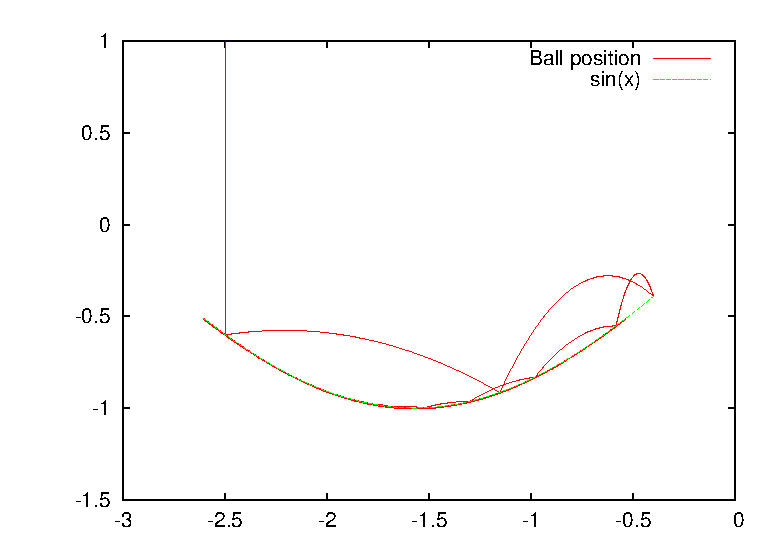
\includegraphics[width=12cm]{ballonsin.eps}
      \caption{Simulation of a ball on a Sine curve}
      \label{ballonsin}
  \end{center}
\end{figure}

\begin{figure}[H]
 \begin{center}
      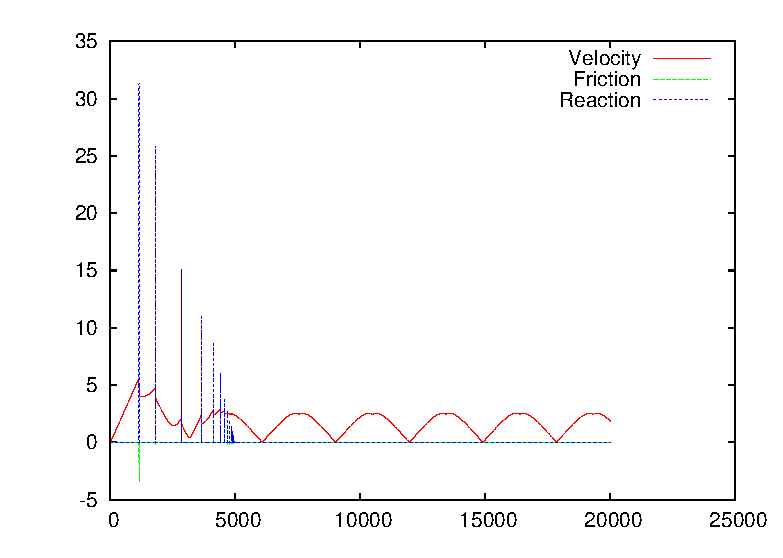
\includegraphics[width=12cm]{ballonsinRFV.eps}
      \caption{Reaction,Friction and velocity}
      \label{ballonsinRFV}
  \end{center}
\end{figure}





Then we are going to do some more complex cases.
We start with a model considering a rover with two wheels, and with friction when a contact happens.
We use Lagrange's equations to create the Dynamical system.
In this system the number of degree of freedom is 5, we use the generalized coordinates $x,y,$ and $\theta$, $\theta_A$, $\theta_B$ to describe the system.

The variables $x$ and $y$ are the location of center of gravity, and $\theta$ is the angle of the rod, $\theta_A$, $\theta_B$ are the angle of the wheel A and B respectively.


The kinetic Energy of the rod is 
\begin{eqnarray}
K_r=\frac{1}{2}m_1(\dot{x}^2+\dot{y}^2)+\frac{1}{2}J_1\dot{\theta}^2
\end{eqnarray}


The velocity of the end of the rod is

\begin{eqnarray}
&v_{rollerA}=\sqrt{(l\dot{\theta}cos\theta+\dot{y})^2+(-l\dot{\theta}sin\theta+\dot{x})^2} \quad \text{At Point A}&\\
&v_{rollerB}=\sqrt{(-l\dot{\theta}cos\theta+\dot{y})^2+(l\dot{\theta}sin\theta+\dot{x})^2} \quad \text{At Point B}&
\end{eqnarray}

The kinetic energy and rotation energy of each roller is

\begin{eqnarray}
\frac{1}{2}m_2v_{roller}^2+\frac{1}{2}J_2\dot{\theta}^2
\end{eqnarray}

The total kinetic energy of the system is
\begin{equation}
\begin{aligned}
K=&\frac{1}{2}m_1(\dot{x}^2+\dot{y}^2)+\frac{1}{2}J_1\dot{\theta}^2\\
&+m_2(l^2\dot{\theta}^2+\dot{y}^2
+\dot{x}^2)+\frac{1}{2}J_2(\dot{\theta_A}^2+\dot{\theta_B}^2)
\label{k1}
\end{aligned}
\end{equation}

We name the center of the front wheel "Wheel B", and the center of the back wheel "Wheel A". The gravity center is O. We write the coordinates of these three points with global coordinate parameters $(x,y,\theta,\theta_A,\theta_B)$

\begin{eqnarray}
&(x_A,y_A)=(x-lcos\theta+rsin\theta_A,y-lsin\theta+rcos\theta_A)& \notag \\
&(x_B,y_B)=(x+lcos\theta+rsin\theta_B,y+lsin\theta+rcos\theta_B)& \notag \\
&(x_O,y_O)=(x,y)& \notag 
\end{eqnarray}

\begin{figure}[htbp]
\begin{center}
\input{Chapter3/pic1.pstex_t} 
\caption{The wheels of the rover  on the ground}
\label{figure:sdd}
\end{center}
\end{figure}

\begin{figure}[htbp]
\begin{center}
\input{Chapter3/pic2_t} 
\caption{Local and Global coordinate system for the wheel}
\label{figure:sdd}
\end{center}
\end{figure}

To compute the generalized forces, we use a transformation of the coordinate system and the equation (\eqref{k3a})
Let's consider the wheel A for example:

\begin{equation}
Q_{k}=\sum_{i=1}^n (F_{xi}\frac{\partial x_{i}}{\partial q_k}+F_{y_i}\frac{\partial y_{i}}{\partial q_k}+F_{zi}\frac{\partial z_{i}}{\partial q_k})
\label{k3a}
\end{equation}

\begin{equation}
\begin{pmatrix}
F_Ax\\F_Ay
\end{pmatrix}=
\frac{1}{\sqrt{k_A^2+1}}\begin{pmatrix}
-k_A & 1\\
1 & k_A \end{pmatrix}
\begin{pmatrix}
\lambda_An \\ \lambda_At
\label{k2a}
\end{pmatrix}
\end{equation}

\begin{equation}
\begin{pmatrix}
R_{Ax}\\ R_{Ay}\\ R_{A\theta} \\R_{A\theta_A}\\ R_{A\theta_B}
\end{pmatrix}=\begin{pmatrix}
1 & 0 \\
0 & 1 \\
lsin\theta & -lcos\theta \\
rcos\theta_A & -rsin\theta_A \\
0 & 0 \end{pmatrix}
\begin{pmatrix}
F_{Ax} \\ F_{Ay}
\label{k1a}
\end{pmatrix}
\end{equation}

Let us substitute \eqref{k2a} into \eqref{k1a}
we obtain the relation from local to global coordinate.

\begin{equation}
\begin{pmatrix}
R_{Ax}\\ R_{Ay}\\ R_{A\theta} \\R_{A\theta_A}\\ R_{A\theta_B}
\end{pmatrix}=\frac{1}{\sqrt{k_A^2+1}}
\begin{pmatrix}
-k_A & 1 \\
1 & k_A \\
 -k_Alsin\theta-lcos\theta & lsin\theta-k_Alcos\theta \\
 -k_Arcos\theta_A-rsin\theta_A & rcos\theta_A-k_Arsin\theta_A\\
0& 0 \end{pmatrix}
\begin{pmatrix}
\lambda_An \\ \lambda_At
\end{pmatrix}
\end{equation}

We use a similar procedure for wheel B
\begin{equation}
\begin{pmatrix}
R_{Bx}\\ R_{By}\\ R_{B\theta} \\R_{B\theta_A}\\ R_{B\theta_B}
\end{pmatrix}=\frac{1}{\sqrt{k_B^2+1}}
\begin{pmatrix}
 -k_B & 1\\
1 & k_B  \\
k_Blsin\theta+lcos\theta & -lsin\theta+k_Blcos\theta\\
0& 0 \\
-k_Brcos\theta_B-rsin\theta_B & rcos\theta_B-k_Brsin\theta_B
 \end{pmatrix}
\begin{pmatrix}
\lambda_Bn \\ \lambda_Bt
\end{pmatrix}
\end{equation}

The generalized force (without external force) is obtained by:

\begin{equation}
F=\begin{pmatrix}
0 \\ -m_1-2m_2 \\ 0 \\0 \\ 0 \end{pmatrix} +R_A+R_B
\end{equation}

We can have Lagrange's equations as follows:
\begin{eqnarray}
&\frac{d}{dt}(\frac{\partial K}{\partial \dot{x}})-\frac{\partial K}{\partial x}=R_{Ax}+R_{Bx}& \label{k2} \\
&\frac{d}{dt}(\frac{\partial K}{\partial \dot{y}})-\frac{\partial K}{\partial y}=-m_1-2m_2+R_{Ay}+R_{By}& \label{k3} \\
&\frac{d}{dt}(\frac{\partial K}{\partial \dot{\theta}})-\frac{\partial K}{\partial \theta}=R_{A\theta}+R_{B\theta}& \\ \label{k4}
&\frac{d}{dt}(\frac{\partial K}{\partial \dot{\theta_A}})-\frac{\partial K}{\partial \theta_A}=R_{A\theta_A}+R_{B\theta_A}&\\
&\frac{d}{dt}(\frac{\partial K}{\partial \dot{\theta_B}})-\frac{\partial K}{\partial \theta_B}=R_{A\theta_B}+R_{B\theta_B}&\\
\end{eqnarray}

We define two functions $d_A(x,y,\theta), \quad d_B(x,y,\theta)$ in the generalized coordinates system to illustrate the nearest distance from the point A and B to the ground surface function $g(x)$

\begin{equation}
  \left\{
   \begin{aligned}
   &d_A(x,y,\theta)\ge 0\\
   &d_B(x,y,\theta)\ge0 \\
   R_A&=0 \quad \text{if $d_A(x,y,\theta)>0$}\\
   R_B&=0 \quad \text{if $d_B(x,y,\theta)>0$} \\
   R_A&>0 \quad \text{if $d_A(x,y,\theta)=0$}\\
   R_B&>0 \quad \text{if $d_B(x,y,\theta)=0$}\\
   f_A&=\mu R_A\\
   f_B&=\mu R_B 
   \end{aligned}
  \right.
  \end{equation}

Substitude equation\eqref{k1} into equation \eqref{k2},\eqref{k3},\eqref{k4}, we have 
\begin{eqnarray}
&m_1\ddot{x}=R_{Ax}+R_{Bx}& \\
&m_1\ddot{y}=-m_1g-2m_2g+R_{Ay}+R_{By}&\\
&J_1+2l^2m_2=R_{A\theta}+R_{B\theta}&\\
&J_2\ddot{\theta_A}=R_{A\theta_A}+R_{B\theta_A}&\\
&J_2\ddot{\theta_B}=R_{A\theta_B}+R_{B\theta_B}&
\end{eqnarray}

In matrix form, we get:
\begin{equation}
q=\begin{pmatrix}
x\\y\\ \theta \\ \theta_A \\ \theta_B
\end{pmatrix}, 
\end{equation}

\begin{equation}
\begin{pmatrix} m_1+2m_2 & 0 & 0 & 0 & 0\\
               0 & m_1+2m_2 & 0 & 0 & 0\\
               0 & 0 & J_1+2l^2m_2& 0 & 0\\
               0& 0& 0& J_2 & 0 \\
               0 & 0 & 0& 0& J_2
\end{pmatrix}\ddot{q}=F,
\end{equation}

with the relations,

\begin{eqnarray}
&h_1(q)=d_A(x,y,\theta)& \\
&h_2(q)=d_B(x,y,\theta)&\\
&H_1=\frac{1}{\sqrt{k_A^2+1}}
\begin{pmatrix}
-k_A &1 \\
1 & k_A \\
 -k_Alsin\theta-lcos\theta & lsin\theta-k_Alcos\theta \\
 -k_Arcos\theta_A-rsin\theta_A & rcos\theta_A-k_Arsin\theta_A\\
0& 0 \end{pmatrix}&\\
&H_2=\frac{1}{\sqrt{k_B^2+1}}
\begin{pmatrix}
 -k_B & 1\\
1 & k_B  \\
k_Blsin\theta+lcos\theta & -lsin\theta+k_Blcos\theta\\
0& 0 \\
-k_Brcos\theta_B-rsin\theta_B & rcos\theta_B-k_Brsin\theta_B
 \end{pmatrix}&
\end{eqnarray}


With a similar method, we can write the equations for a ball to ball contact, which could describe the contact between the wheel and the sand. Using the multibody tools in Siconos, we can inject small disks automatically. The multibody tool enable us to simulate the Rover on granular soil in 2D\footnote{Source File Location: siconos/trunk/SandBox/Rover/RoverDisks} Fig\eqref{ROVER2D}:\\


In this case, we use small disk to simulate the granular soil, the relations between the disks will be generated automatically when any two disks are close to each other. And during the simulation, the SpaceFilter class will detect the distance between disks with relations, if they become far from each other, this class will remove the relation, to reduce the memory use and computing cost.


\begin{figure}[H]
 \begin{center}
      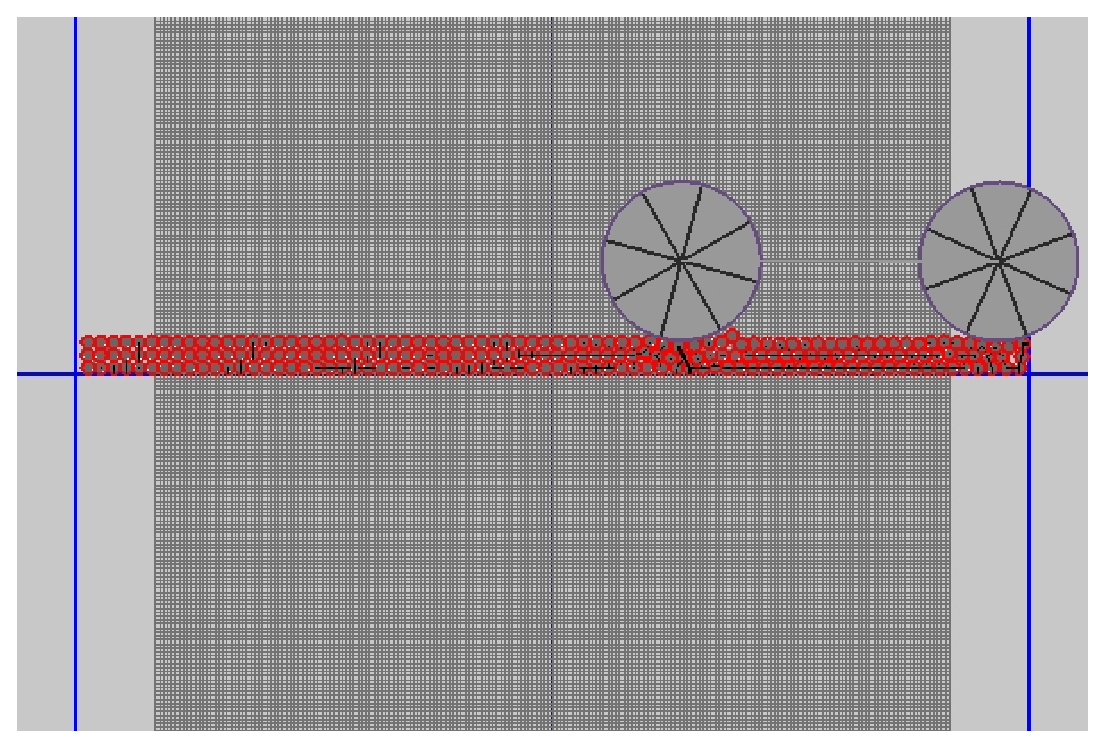
\includegraphics[width=8cm]{toto-0076.EPS}
      \caption{Rover on granular soil in 2D}
      \label{ROVER2D}
  \end{center}
\end{figure}


\section{Extension to 3D model}

For 3D Rover modeling, the inertia matrix and contact model interaction relation will be very complex. So, we can write a Maple code to generate this relations automatically, and export into C files. In our Siconos code, we can import this relations as a plug-in function. The Maple code enable us to easily do complex modeling easily with high accuracy. \\

The software HuMAns developed by team Bipop is used to generate the dynamical model for the Rover. In the software HuMAns, we need to create several maple input files to indicate the relative location of key-points of the model and the degree of freedom of every connecting point. \\

However, HuMAns is designed for the Robotics dynamic system and contact. In the HuMAns the contact model is for flat plane contact. In the case of Rover, more complex contact model is required to describe the phenomenon. Our simulation should be able to simulate the motion of Rover on uneven ground. So an improvement of HuMAns is required.

A typical dynamic system can be set in the form:
$$
M(q) \ddot{q} + N(q,\dot{q}) \dot{q} + G(q) = T(q) u
$$
where $q$ is the system state variable, $M(q)$ the system inertia,
$N(q,\dot{q})$ a non-linear effects matrix, $G(q)$ the forces which derived from a potential energy (for example the gravity), $u$ a command vector and a matrix
describing the effect of this command on the system. \\ 

When the Rover is moving on the ground, the Rover is support by some contact points between the tyres and the soil. Howewer, so we need to develop a contact model to describe the dynamic of a system
with these constraints.\\

So we have a set of inequalities on the position
of the model (the robot or the human), that is, on the state vector
$q$:
$$
\varphi_n(q) \geq 0
$$
If we consider the points in contact with the environment at time $t$
and if we indicate them with an $*$, we can write:
$$
\varphi_n^*(q) = 0
$$


The aim of using HuMAns is to generate the Matrix $M(q)$, $N(q,\dot{q})$, $G(q)$, $T(q)$ , $\varphi_n(q)$ as well as $\frac{\partial \varphi_n(q)}{\partial q}$automatically. Then, this dynamical model could be used in the simulation of Siconos.

%\section{Future work}
%
%This internship is still going on. The HuMAns improvement has been done, and the verification of this new version has also been done. With the %%guide of my supervisor, we will put this model in real 3D atmosphere, with small balls, and also link our code with 3DROV from Trasys to %improve the capability of 3DROV.







\chapter{Details of model creation and computing}
\section{Rover3D model creation with Maple}

A Maple code package will be created to generate the dynamical system of the Rover %(in the  figure). 
and C files for visualization.


\subsection{Kinematic data and Geometry description of Rover}

We used the Cardan representation for the Rover model.\\

% insert the coordinate system figures.

The description of the dynamical data of the Rover is composed with "solids". "Solids" are linked with each other using vectors. An $(O_k, X_k, Y_k, Z_k)$ frame is attached to each solid $k$. The position and the orientation of the frame $k$ is given in the frame $ref_k$ of the solid it is attached to. So we need six parameters to describe a new "solid". A translation $(Tx_k, Ty_k, Tz_k)$ and a rotation of $z_k$ around
$z_{ref_k}$ (roll), a rotation of $y_k$ around the resulting $y$-axis (pitch) and finally a rotation of $x_k$ around the resulting $x$-axis
(yaw) should be included in the Dynamical data file for Maple code. \\

The figure \eqref{RoverSketup} will show us the geometry of Rover and describes what is "solids" and relationship between each other. A part of the \textbf{KinematicData.maple} input file is given to illustrate the structure of the dynamic data description. \footnote{The 3D model file in Google Sketchup format could found in: /home/bipop/jyang/siconos/trunk/SandBox/Rover}\\

\begin{figure}[H]
 \begin{center}
      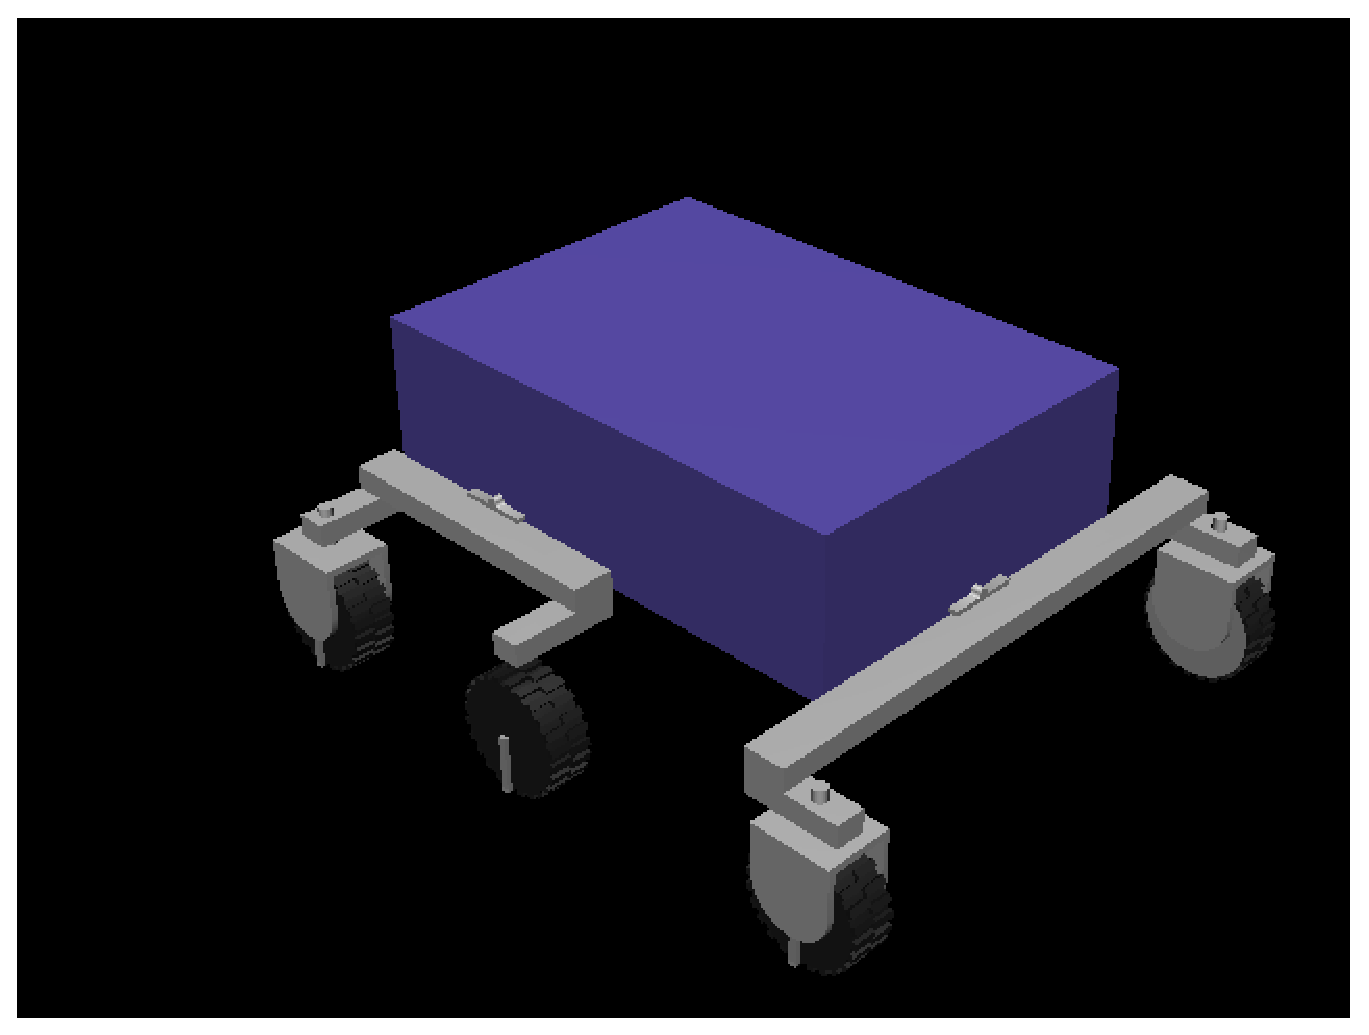
\includegraphics[width=3in]{Chapter4/rovereps.eps}
    \caption{Geometry of Rover}
  \end{center}
\label{RoverSketup}
\end{figure}


% insert the kinematic system figures.
\begin{figure}
\begin{center}
 \input{Chapter4/kinematic1.pstex_t}
\caption{Articular notations of Rover}
\end{center}
\end{figure}


\begin{figure}[!h]
\begin{minipage}[t]{.6\linewidth}
\begin{center}
\begin{tiny}
\begin{verbatim}
# solids number
NSOL := 16:

# degrees of freedom number
NDDL := 21:

#generalized coordinates and velocity definition
q := vector(NDDL):
qdot := vector(NDDL):

# l = vector of mechanical lenghts


#Cardan Rotation: We begin with the rotation around z, then around y then
#around x

# Frame 1 : Mass center: Orientation and position
ref_1	:= 0:
z_1 := q[6]:   #rotation along x,y,z aixs
y_1 := q[5]:
x_1 := q[4]:
Tx_1 := q[1]:  #location of the rover
Ty_1 := q[2]:
Tz_1 := q[3]:

# Frame 2 : Axle F (Front)
ref_2	:= 1:
z_2	:= 0:
y_2	:= 0:
x_2	:= q[7]:  #have a rotation freedom in x direction
Tx_2	:= 62:    #translation vector from its reference solid (solid 1)
Ty_2	:= -10:  
Tz_2	:= 0:

# Frame 3 : Steering Axle FL (Front Left)
ref_3	:= 2:
z_3	:= 0:
y_3	:= q[8]:  #Have a roataion degree of freedom in y direction
x_3	:= 0:    
Tx_3	:= 0:     #translation vector from its reference solid(Solid 2)
Ty_3	:= 0:
Tz_3	:= -53:

.
.
.
\end{verbatim}
\end{tiny}
\end{center}
\end{minipage}
\hfill
\begin{minipage}[t]{.4\linewidth}
\begin{center}
\begin{tiny}
\begin{verbatim}
.
.
.

# Frame 14 : Steering Axle BR 
ref_14	:= 12:
z_14	:= 0:
y_14	:= q[19]:
x_14	:= 0:
Tx_14	:= -30:
Ty_14	:= 0:
Tz_14	:= 0:

# Frame 15 : Wheel MR 
ref_15	:= 13:
z_15	:= q[20]:
y_15	:= 0:
x_15	:= 0:
Tx_15	:= 0:
Ty_15	:= -15:
Tz_15	:= 0:

# Frame 16 : Wheel BR 
ref_16	:= 14:
z_16	:= q[21]:
y_16	:= 0:
x_16	:= 0:
Tx_16	:= 0:
Ty_16	:= -15:
Tz_16	:= 0:

\end{verbatim}
\end{tiny}
\end{center}
\end{minipage}
\caption{Part of \textbf{KinematicData.maple} file which describes the
  position and the orientation of a jointed model with the
  yaw-pitch-roll angles.}
\label{fig:LagMod-CarAngKinematicData}
\end{figure}

With \textbf{KinematicData.maple}, the maple code knows the translation and rotation information between nodes. The table will describe all the name of nodes(Solids) and its degree of freedom and location in local frame.
 
\newcommand{\tabincell}[2]{\begin{tabular}{@{}#1@{}}#2\end{tabular}}
\begin{table}[htbp]
\begin{center}
\begin{tabular}{lccccc}
  \toprule
   No. & Name   & Ref. No. & \tabincell{c}{Rotation\\freedom} & \tabincell{c}{Location in\\Ref fram} & Description\\
  \midrule
  1 &Mass center & Non & $x,y,z$ & $(0,0,0)$ & \tabincell{c}{The mass center\\of the Rover, 6 DOF}\\
  2&Axle F  & 1 &  $x$ & $(62,-10,0)$ & The pivot at the front \\
  3&\tabincell{c}{Steering\\ Axle FL} & 2 & $y$ & $(0,0,-53)$ & \tabincell{c}{Steering Axle\\ at the front left side}\\
  4&\tabincell{c}{Steering\\ Axle FR} & 2 & $y$ & $(0,0,53)$ & \tabincell{c}{Steering Axle\\ at the front right side}\\
  5&Wheel FL & 3 & $z$ & $(0,-15,0)$ & \tabincell{c}{Rover Tire at the\\ front left side}\\
  6&Wheel FR & 4 & $z$ & $(0,-15,0)$ & \tabincell{c}{Rover Tire at the\\ front right side}\\
  7&Axle BL  & 1 &  $z$ & $(-40,-10,-53)$ & \tabincell{c}{The pivot at\\ left side} \\
  8&\tabincell{c}{Steering\\ Axle ML} & 7 & $y$ & $(30,0,0)$ & \tabincell{c}{Steering Axle at\\the middle of left side}\\
  9&\tabincell{c}{Steering\\ Axle BL} & 7 & $y$ & $(-30,0,0)$ & \tabincell{c}{Steering Axle at\\the back of left side}\\
  10&Wheel ML & 8 & $z$ & $(0,-15,0)$ & \tabincell{c}{Rover Tire at the\\middle of left side}\\
  11&Wheel BL & 9 & $z$ & $(0,-15,0)$ & \tabincell{c}{Rover Tire at the\\back of left side}\\
  12&Axle BR  & 1 &  $z$ & $(-40,-10,53)$ & \tabincell{c}{The pivot at\\ right side} \\
  13&\tabincell{c}{Steering\\ Axle MR} & 12 & $y$ & $(30,0,0)$ & \tabincell{c}{Steering Axle at\\the middle of right side}\\
  14&\tabincell{c}{Steering\\ Axle BR} & 12 & $y$ & $(-30,0,0)$ & \tabincell{c}{Steering Axle at\\the back of right side}\\
  15&Wheel MR & 13 & $z$ & $(0,-15,0)$ & \tabincell{c}{Rover Tire at the\\middle of right side}\\
  16&Wheel BR & 14 & $z$ & $(0,-15,0)$ & \tabincell{c}{Rover Tire at the\\back of right side}\\


  \bottomrule
 \end{tabular}
\caption{Kinematic Data of the Rover}
\end{center}
\end{table}


Some characteristic points which we are interested could be defined as tags. We create a maple file \textbf{AdditionnalData.maple} to describe the location of Tags. The data describing location tags could be composed as two part: 
\begin{itemize}
\item The Number of Ref solid the tag is attached to
\item One vector describing the translation from this Solid point
\end{itemize}

\begin{figure}[!h]
\begin{minipage}[t]{.6\linewidth}
\begin{center}
\begin{tiny}
\begin{verbatim}
# Definition de quelques points importants (tags)

# Tag 1 : Mass center
reftag_1 := 1:           #Ref Number which the tag is attached to
tag_1    := vector([0,0,0]):  #vector from this Solid

# Tag 2 : Pivot F
reftag_2 := 2:
tag_2    := vector([0,0,0]):
.
.
.

\end{verbatim}
\end{tiny}
\end{center}
\end{minipage}
\caption{Part of \textbf{AdditionnalData.maple} file which describes the
  positions of the tags in their attached segment frame.}
\label{fig:LagMod-AdditionnalData}
\end{figure}


The main Maple code \textbf{ModelGeneration.maple} will generate a C file \textbf{Tags.c} with the data in \textbf{AdditionnalData.maple}.
This C file enable us to get the global coordinate data of all the Tags. In order to use this C file to compute the coordinates. We need to input the state vector q as well as a null matrix T which will be used for output. \\

$T$ is on the form:
$$
T = 
\left(
\begin{array}{ccc}
x_{tag_1}^{0} & y_{tag_1}^{0} & z_{tag_1}^{0} \\
x_{tag_2}^{0} & y_{tag_2}^{0} & z_{tag_2}^{0} \\
\vdots & \vdots & \vdots \\
x_{tag_{NumberOfTags}}^{0} & y_{tag_{NumberOfTags}}^{0} &
z_{tag_{NumberOfTags}}^{0} \\
x_{CenterOfMass}^{0} & y_{CenterOfMass}^{0} & z_{CenterOfMass}^{0} \\
\end{array}
\right)
$$
where the $0$ represents the reference frame. 

\subsection{Dynamical data input}
The inertials parameters (the gravity vector, the mass of the segment, the position of
the segments centers of mass and the inertia matrix of these segments
relative to the centers of their attached frames) are defined in the file \textbf{DynamicData.maple}. The
figure \ref{fig:LagMod-DynamicData} shows an example of this file. 

\begin{figure}[H]
\begin{minipage}[t]{.6\linewidth}
\begin{center}
\begin{tiny}
\begin{verbatim}

#dynamic data for Rover3D

# Gravity vector
Gravity := vector([0, -9.81, 0]):


# solid size matrix (a,b,c) on (x,y,z) in meters unity
sizematrix := [[120,40,100], #  trunk: Orientation and position
               [6,6,115],    #  Axle F (Front) 			
               [3,15,0],     #	Steering Axle FL (Front Left)	
               [3,15,0],     #  Steering Axle FR (Front Right)	
               [10,0,0],     #  Wheel FL		
               [10,0,0],     #  Wheel FR			
               [70,6,6],     #  Axle BL				
               [3,15,0],     #  Steering Axle ML  		
               [3,15,0],     #  Steering Axle BL  	
               [10,0,0],     #  Wheel ML 			
               [10,0,0],     #  Wheel BL 			
               [70,6,6],     #  Axle BR
               [3,15,0],     #  Steering Axle MR 		
               [3,15,0],     #  Steering Axle BR 		
               [10,0,0],     #  Wheel MR       			
               [10,0,0]]:    #	Wheel BR       			


# Rover total mass in kilogrammes unity
Mass := 1:	


# solid mass matrix in rate of total mass
massmatrix := [600,   #  trunk: Orientation and position
               50,    #  Axle F (Front)
               5,     #	 Steering Axle FL (Front Left)
               5,     #  Steering Axle FR (Front Right)
               30,    #  Wheel FL
               30,    #  Wheel FR
               50,    #  Axle BL
               5,     #  Steering Axle ML 
               5,     #  Steering Axle BL 
               30,    #  Wheel ML
               30,    #  Wheel BL 
               50,    #  Axle BR
               5,     #  Steering Axle MR 
               5,     #  Steering Axle BR 
               30,    #  Wheel MR 
               30]*1:   #	 Wheel BR 

MatHuygens := proc(G) option remember;

	RETURN(matrix([[G[3]^2+G[2]^2, -G[2]*G[1], -G[3]*G[1]],
		[-G[2]*G[1], G[3]^2+G[1]^2, -G[3]*G[2]],
		[-G[3]*G[1], -G[3]*G[2], G[2]^2+G[1]^2]])):
end:


# function created to compute the inertia matrix

IOMatrix := proc(k) option remember;
local mk, IG, Gk;
	
	mk := Mass * massmatrix[k]:
	IG := matrix([[mk*(sizematrix[k,3]^2 + sizematrix[k,2]^2) /12, 0, 0],
		      [0, mk*(sizematrix[k,1]^2 + sizematrix[k,3]^2) /12, 0],
		      [0, 0, mk*(sizematrix[k,1]^2 + sizematrix[k,2]^2) /12]]):
	Gk := G_||(k):
	RETURN(evalm(IG + mk*MatHuygens(Gk))):	
end:


.
.
.
\end{verbatim}
\end{tiny}
\end{center}
\end{minipage}
\hfill
\begin{minipage}[t]{.4\linewidth}
\begin{center}
\begin{tiny}
\begin{verbatim}
.
.
.

#Inertia matrix for Disk
IOMatrixDisk :=proc(k) option remember;
local mk , r, IG;
      mk := Mass*massmatrix[k]:
      r  := sizematrix[k,1]:
      IG := matrix([[mk*r^2/4, 0, 0],
		      [0,mk*r^2/4, 0],
		      [0, 0,mk*r^2/2 ]]):
      RETURN(IG):	
end:

#Inertia matrix for Cylinder
IOMatrixCylinder := proc(k) option remember;
local mk, r, h, IG;
       mk :=Mass*massmatrix[k]:
       r  := sizematrix[k,1]:
       h  := sizematrix[k,2]:
       IG := matrix([[mk*(3*r^2+h^2)/12,0,0],
                     [0,mk*r^2/2,0],
                     [0,0,mk*(3*r^2+h^2)/12]]):
       RETURN(IG):
end:


# Solid 1 : trunk: Orientation and position
m_1  := massmatrix[1]*Mass:
G_1  := vector([0, 0, 0]):
IO_1 := IOMatrix(1):


# Solid 2 : Axle F (Front)
m_2  := massmatrix[2]*Mass:
G_2  := vector([0, 0, 0]):
IO_2 := IOMatrix(2):


# Solid 3 : Steering Axle FL (Front Left)
m_3  := massmatrix[3]*Mass:
G_3  := vector([0, 0, 0]):
IO_3 := IOMatrixCylinder(3):


# Solid 4 : Steering Axle FR (Front Right)
m_4  := massmatrix[4]*Mass:
G_4  := vector([0, 0, 0]):
IO_4 := IOMatrixCylinder(4):


# Solid 5 : Wheel FL
m_5  := massmatrix[5]*Mass:
G_5  := vector([0, 0, 0]):
IO_5 := IOMatrixDisk(5):


# Solid 6 : Wheel FR
m_6  := massmatrix[6]*Mass:
G_6  := vector([0, 0, 0]):
IO_6 := IOMatrixDisk(6):



\end{verbatim}
\end{tiny}
\end{center}
\end{minipage}
\caption{The \textbf{DynamicData.maple} file describes different
  inertial parameters of the model.}
\label{fig:LagMod-DynamicData}
\end{figure}

In this maple file, we could define:

\begin{itemize}
\item The gravity vector (defined in vector Gravity)
\item The geometry of every segment (defined in Matrix sizematrix, length, height,width,radius etc)
\item Mass of each segment (defined in the Matrix massmatrix)
\item Mass center of the segment (defined in \verb|G_i|, i is the solid number), and the function MatHuygens will be called to do the translation if the mass center is not at the geometry center.
\item Inertia matrix is defined in the function IOMatrix,IOMatrixDisk,IOMatrixCylinder, which are for inertia matrix computing of rectangle,disk and cylinder respectively.
\end{itemize}

The \textbf{ModelGeneration.maple} file contains:

\begin{itemize}
\item \textbf{GenerateInertiaMatrix} procedure which uses the \textbf{InertiaRecursion} function to generate the \textbf{Inertia.c}
file.
\item \textbf{GenerateNLEffectsVector} procedure which uses the \textbf{NLEffectsRecursion} function to generate the
\textbf{NLEffects.c} file
\end {itemize}


\chapter{Contact Description}

To describe the contact of the Rover with the solid ground or granular soil in Siconos, we need two plugin functions:
\begin{itemize}
\item $h$ function to compute the distance between contact points
\item $G$ is the transformation matrix of velocity of contact points from the global frame to the local frame
\end{itemize}
To simplify the model, we only consider point contact. In this contact model, we simplify the axis of the wheel into a point, and create contact model between this point and the sphere or plane.
  

\section{Computation of distance}
\subsection{Wheel/Plane Contact}
With the use of Tags.c file, we can get all the coordinates of tags. In \textbf{AdditionnalData.maple}, we set some points on the tyres as tags, from which we can get the coordinates. Consider tyre plane contact in Fig \eqref{WHcontact}, $E$ is the contact point. Assume the plane equation is $Ax+By+Cz+D=0$, the length of line $EF$ is the distance we want for the contact model.

\begin{figure}[H]
\begin{center}
 \input{Chapter4/contactplane.pstex_t}
\caption{Wheel/Plane Contact}
\label{WHcontact}
\end{center}
\end{figure}

The algorithm for computing distance could be summarized as flowing steps.

\begin{itemize}
\item Vector $\vec{s}$ is a unit vector perpendicular to the tyre. In order to get this vector, we set this vector as a tag in \textbf{AdditionnalData.maple}. Then it is possible to obtain this vector from \textbf{Tags.c}.
\item Vector $\vec{n}_{plane}$ is a vector perpendicular the plane. It is obtained from the plane equation $Ax+By+Cz+D=0$: $\vec{n}_{plane}=(A,B,C)$
\item The vector pointing the moving direction of tyre $\vec{m}$ could be obtained by cross product of  $\vec{s}$ and $\vec{n}_{plane}$, $\vec{m}=\vec{n}_{plane} \times \vec{s}$
\item Vector $\vec{t}$ is the normalized vector of $\vec{m}$.
\item The normal vector of local frame $\vec{n}$ could be obtained from the cross product of $\vec{t}$ and $\vec{s}$: $\vec{n}=\vec{s} \times \vec{t}$.
\item The vector pointing to the contact point $\overrightarrow{GE}=-R\vec{n}$. Where $R$ is the radius of the tyre.
\item The coordinates of contact point $E$ could be obtain by vector operation: $\overrightarrow{OE}=\overrightarrow{OG}+\overrightarrow{GE}$.
\item The value of distance could be obtained by using distance formulation \eqref{DistanceFormulation} 
\end{itemize}


\begin{eqnarray}
d= \frac{\left| Ax+By+Cz+D \right|}{\sqrt{A^2+B^2+C^2}}
\label{DistanceFormulation}
\end{eqnarray}

We make a function $ContactDistance$ in \textbf{ModelGeneration.maple} to compute the distance of six contact points and save the result in a vector. The vector will be export as a C file \textbf{Distance.c}. To use this C file, we need to input the state vector $q$, and four parameter vector $P=(A,B,C,D)$ of the plane, as well as a Null vector $distance$ which the result will be saved to. The general format is \textbf{Distance(distance,P,q)}.\\

And during the computing of the contact distance, local frame is also obtained: $(\vec{s},\vec{t},\vec{n})$.

\subsection{Wheel/Sphere Contact}

\begin{figure}[H]
\begin{center}
 \input{Chapter4/contactsphere.pstex_t}
\caption{Wheel/Sphere Contact}
\label{Wheel/Sphere Contact}
\end{center}
\end{figure}


In Wheel/Sphere distance computation, flowing steps are used to obtain the contact distance.

\begin{itemize}
\item With similar method used in Wheel Plane contact, we can obtain the vector $\vec{s}$ which is perpendicular to the tyre by defining a tag in \textbf{AdditionnalData.maple}.
\item Assum $\vec{s}=(A,B,C)$ and the coordinates of point $D$ is $\overrightarrow{OD}=(x_0,y_0,z_0)$, we can write the tyre plane equation as $Ax+By+Cz=Ax_0+By_0+Cz_0$.
\item The distance between the sphere and the tyre plane $\left| \overrightarrow{AB} \right|$ could be obtained by formulation \eqref{DistanceFormulation}. 
\item \begin{eqnarray}
      &\overrightarrow{AB}=-\left| \overrightarrow{AB} \right| \overrightarrow{s}& \\
      &\overrightarrow{OB}=\overrightarrow{OA}+\overrightarrow{AB}& \\
      &\overrightarrow{DB}=\overrightarrow{OB}-\overrightarrow{OD}& \\
      &\overrightarrow{DC}=\frac{\overrightarrow{DB}}{\left| \overrightarrow{DB} \right|}R& \quad \text{where $R$ is the radius of the tyre}\\ 
      &\overrightarrow{OC}=\overrightarrow{OD}+\overrightarrow{DC}&
      \end{eqnarray}
\item With the coordinates of point $C$, the contact distance is obtained by $\left| \overrightarrow{OA}-\overrightarrow{OC} \right|-R_s \quad$ where $R_s$ is the radius of the sphere. 
\item What's more, we can obtain the local fram vector $\vec{n}=-\frac{\overrightarrow{DC}}{\left| \overrightarrow{DC} \right|}$ , $\vec{t}=\vec{n} \times \vec{s}$
\end{itemize}

\section{$G$ function computation}

To construct the local velocity frame, we need local coordinate system $(\vec{s},\vec{t},\vec{n})$ \\


With the local frame $(\vec{s},\vec{t},\vec{n})$, we could use matrix $[\vec{s},\vec{t},\vec{n}]$ as rotation matrix to transform the global velocity to local frame.\\

In order to get the velocity in local frame, we start from the global coordinates. Function ContactVector in \textbf{ModelGeneration.maple} could give the coordinates of contact points for us. They are functions of state vector $q$: 

\begin{eqnarray}
P_{global}=\begin{pmatrix}
x(q)\\
y(q)\\
z(q)
\end{pmatrix}
\end{eqnarray}

And we have velocity in global frame:

\begin{eqnarray}
v_{global}=\frac{dP_{global}}{dt}=
\begin{pmatrix}
\frac{dx(q)}{dt}\\
\frac{dy(q)}{dt}\\
\frac{dz(q)}{dt}
\end{pmatrix}=
\begin{pmatrix}
\nabla_{q}x\\
\nabla_{q}y\\
\nabla_{q}z
\end{pmatrix}\dot{q}
\end{eqnarray}

And we can get the velocity in local frame by multiplying the rotation matrix $T=[\vec{s},\vec{t},\vec{n}]$

\begin{eqnarray}
v_{local}=Tv_{global}=T\begin{pmatrix}
\nabla_{q}x\\
\nabla_{q}y\\
\nabla_{q}z
\end{pmatrix}\dot{q}=G\dot{q}
\end{eqnarray}

The matrix $G=T(\nabla_{q}x,\nabla_{q}y,\nabla_{q}z)^T$ is what we need in Siconos relation definition.

The computing procedure of matrix $G$ is in function ContactJacobianMatrix of file \textbf{ModelGeneration.maple}


\subsection{Consideration of thickness of the wheels}

The model for computing the distance is for the wheels without thickness, or very "thin" wheels. Now, we develop the model with consideration of thickness. \\


In the previous section, we have found the contact point of thin wheel, and assume the coordinates is $\overrightarrow{OA}$. We can prove that all the possible contact point $B$ on the wheel could be written as $\overrightarrow{OB}=\overrightarrow{OA}+k\vec{s}$, where $\vec{s}$ is the unite vector normal to the wheel plane. And $-\frac{t}{2}\le k \le \frac{t}{2}, \quad t \quad \text{is the thickness of the wheel}$.

\begin{figure}[H]
\begin{center}
 \input{Chapter4/thickness.pstex_t}
\caption{Model with consideration of thickness}
\label{Thickness}
\end{center}
\end{figure}

And function $f(\overrightarrow{OB})$ compute the distance between the contact points. The contact distance with consideration of thickness could be written as: $h(q)=minimize_{k} \quad f(\overrightarrow{OB}=\overrightarrow{OA}+k\vec{s})$.\\

In the Maple software, the computing time of analytical solution is not acceptable. A numerical approximation is implemented in the code. We export the analytical solution of distance $f(\overrightarrow{OA}+k\vec{s})$ in C file. In this C file, $k$ is keep as symbol. In the C++ class \textbf{Rover3DWheelFixedSphereR}, the interval $-\frac{t}{2}\le k \le \frac{t}{2}$ is divided into smaller intervals with same size. We only compute distances these points with spheres, and the shortest distances is selected as the contact distance.


\begin{equation}
h(q)= \underset{-\frac{t}{2}\le k \le \frac{t}{2}}{\text{minimize}}\quad f(\overrightarrow{OB}=\overrightarrow{OA}+k\vec{s})
\end{equation}


Where $k$ is the thickness of the wheel.
\section{PID controller}



A PID controller(proportional–integral–derivative controller) is used for the steering system of the rover.
Siconos enable us to put PID controller easily by plugging a external force term  $F_{Ext}(t,z)$ in the Lagrangian Non Linear Dynamical System. \ref{LNLDS}

\begin{equation}
M(q,z)\ddot{q}+NNL(\dot{q},q,z)+F_{Int}(\dot{q},q,t,z)=F_{Ext}(t,z)+p
\label{LNLDS}
\end{equation}

A typical PID control scheme is composed with three correcting terms in order to minimize the difference between  process variable(SP) and setpoint (PV):
\begin{equation}
MV(t)= P_{out} +I_{out}+ D_{out}
\end{equation}

Where 
\begin{eqnarray}
&P_{out}=K_pe(t)& \\
&I_{out}=K_i\int_0^{t} e(\tau) d\tau&\\
&D_{out}=K_d\frac{d}{dt}e(t)&\\
&K_p,K_i,K_d \quad& \text{tuning parameters}\\
&e(t)=SP-PV& \text{Error}
\end{eqnarray}

In our particular case, we only use two correcting terms $P_{out}$ and $D_{out}$:
\begin{eqnarray}
&P_{out}=K_p(q(i)-q_0(i))&\\
&D_{out}=K_d(v(i)-v_0(i))&
\end{eqnarray}

Where $q(i)$ is the variable we would like control. $q_0(i)$ is the initial value.

Hence, The dynamical system could be describe as:
\begin{equation}
M(q,z)\ddot{q}+NNL(\dot{q},q,z)+F_{Int}(\dot{q},q,t,z)=K_p(q(i)-q_0(i))+K_d(v(i)-v_0(i))+p
\label{LNLDSPID}
\end{equation}

The code for PID controller is include in the file  \textbf{RobotPlugin.cpp}
 


\section{Other useful functions}

To visualize the result in 3D, we need to create a VRML file with the result data. The VRML file use Axis angle rotation representation to describe a rotation, we need to transform our rotation matrix to an axis angle rotation representation when writing the VRML file.This procedure could be found in file \textbf{AdditionnalData.maple}.












\chapter{Numerical Application}
\section{Simulation on the Plane}
\subsection{Initial condition}
We consider a Rover on a incline plane. The rover will be put above the plane as the initial position. Then it will fall freely to the plane. The code will simulate the contact and friction between the tyres and the plane. And driving force is put on six wheels. The two front wheel will turn to the right direction.\footnote{Source File Location: siconos/trunk/SandBox/Rover/Rover3DPlane}
\begin{figure}[H]
 \begin{center}
      
\includegraphics[width=4in]{Chapter5/roverepsplane.eps}
    \caption{Initial condition of RoverPlane model}
  \end{center}
\end{figure}



\subsection{Simulation result}
Beside the VRML animation, we can also export some data to display more details of the movement of the Rover.

\begin{figure}[H]
 \begin{center}
      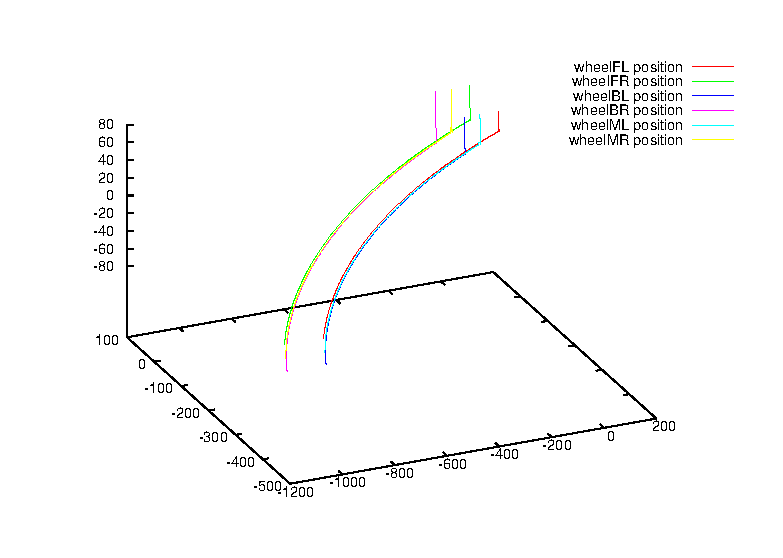
\includegraphics[width=4in]{Chapter5/RoverPlane.eps}
    \caption{Trace of Rover Wheels}
  \end{center}
\end{figure}

\begin{figure}[H]
 \begin{center}
      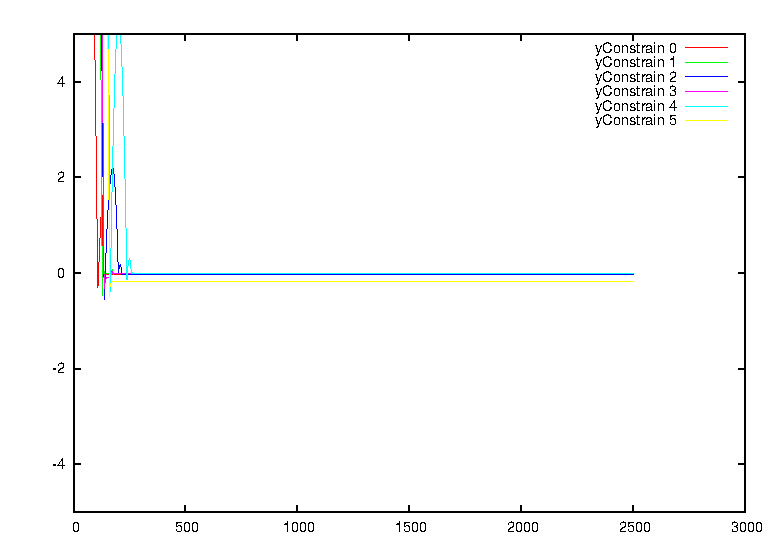
\includegraphics[width=3.5in]{Chapter5/RoverPlaneConstrain.eps}
    \caption{Contact Distance between Wheels and Plane}
    \label{RoverPCons}
  \end{center}
\end{figure}

In the figure \ref{RoverPCons}, we can find that, all the wheels are constrained upon the plane very well.

\begin{figure}[H]
 \begin{center}
      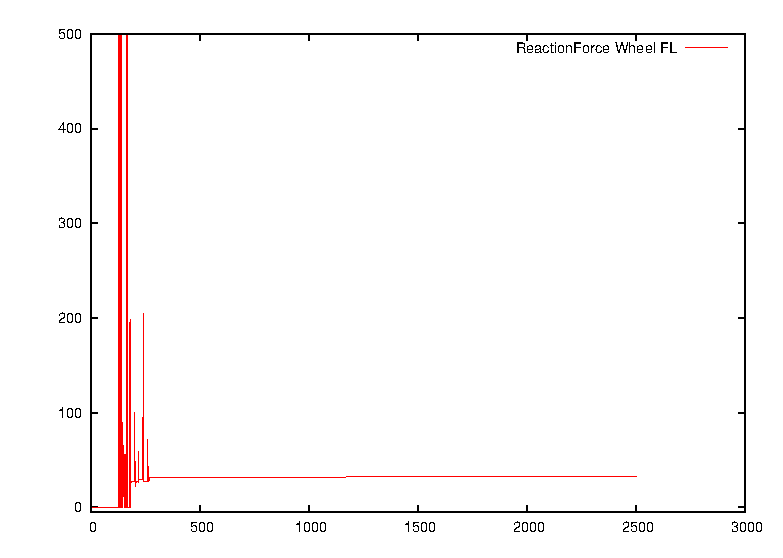
\includegraphics[width=3in]{Chapter5/RoverPlaneReaction.eps}
    \caption{Reaction force of Front Left Wheel}
  \end{center}
\end{figure}

\begin{figure}[H]
 \begin{center}
      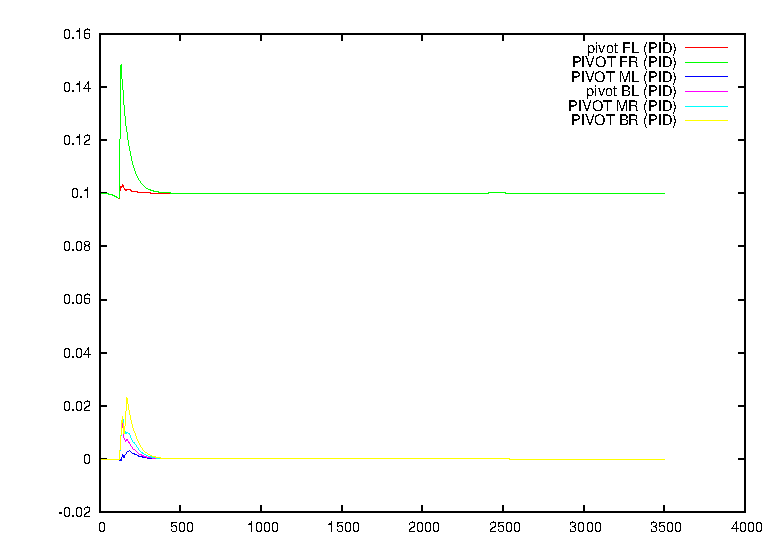
\includegraphics[width=3in]{Chapter5/RoverPlanePID.eps}
    \caption{PID controller}
    \label{PIDfig}
  \end{center}
\end{figure}

Fig \eqref{PIDfig} record the angle of steering system along with time. From the curve,we can find that, the PID controller constrain the steering angle very well.

\section{Simulation on Fixed Spheres}
To simulate Mars Rover on the granular soil, we could use spheres to simulate the granular soil. The figure below shows the simulation of Rover with fixed spheres, to test the validity of our dynamical model.\footnote{Source Files Location: siconos/trunk/SandBox/Rover/Rover3D\_Multi\_Sphere}


\begin{figure}[H]
 \begin{center}
      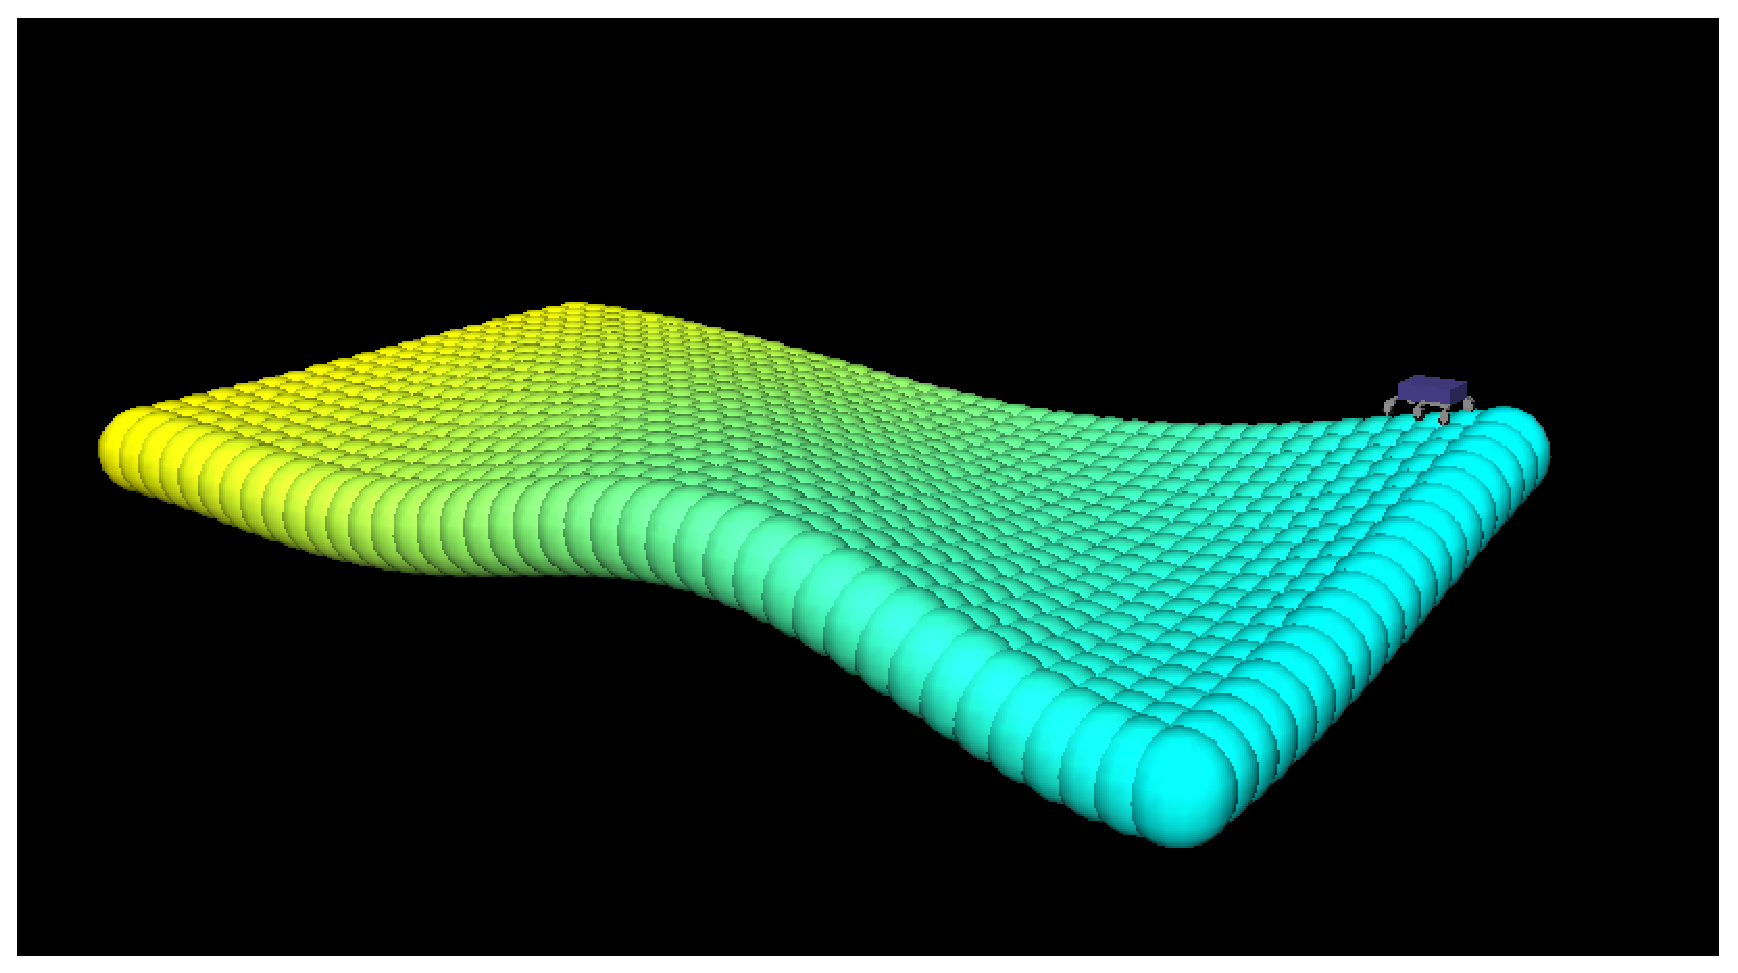
\includegraphics[width=5in]{Chapter5/RoverSpheres.eps}
    \caption{Simulation of Rover with fixed Sphere}
  \end{center}
\end{figure}




%\include{Conclusions/conclusions}

%\appendix
%\include{Appendix1/appendix1}




%\bibliographystyle{Classes/CUEDbiblio}
%\bibliographystyle{Classes/jmb}
%bibliographystyle{plainnat} %this works with package natbib
%\bibliographystyle{plain} % bibliography style
%\renewcommand{\bibname}{References} % changes default name Bibliography to References
%\bibliography{References/references} % References file



%\addcontentsline{toc}{chapter}{References} %adds References to contents page
%\include{Acknowledgement/acknowledgement}
\end{document}
